% Options for packages loaded elsewhere
\PassOptionsToPackage{unicode}{hyperref}
\PassOptionsToPackage{hyphens}{url}
\PassOptionsToPackage{dvipsnames,svgnames,x11names}{xcolor}
%
\documentclass[
  letterpaper,
  DIV=11,
  numbers=noendperiod]{scrartcl}

\usepackage{amsmath,amssymb}
\usepackage{iftex}
\ifPDFTeX
  \usepackage[T1]{fontenc}
  \usepackage[utf8]{inputenc}
  \usepackage{textcomp} % provide euro and other symbols
\else % if luatex or xetex
  \usepackage{unicode-math}
  \defaultfontfeatures{Scale=MatchLowercase}
  \defaultfontfeatures[\rmfamily]{Ligatures=TeX,Scale=1}
\fi
\usepackage{lmodern}
\ifPDFTeX\else  
    % xetex/luatex font selection
\fi
% Use upquote if available, for straight quotes in verbatim environments
\IfFileExists{upquote.sty}{\usepackage{upquote}}{}
\IfFileExists{microtype.sty}{% use microtype if available
  \usepackage[]{microtype}
  \UseMicrotypeSet[protrusion]{basicmath} % disable protrusion for tt fonts
}{}
\makeatletter
\@ifundefined{KOMAClassName}{% if non-KOMA class
  \IfFileExists{parskip.sty}{%
    \usepackage{parskip}
  }{% else
    \setlength{\parindent}{0pt}
    \setlength{\parskip}{6pt plus 2pt minus 1pt}}
}{% if KOMA class
  \KOMAoptions{parskip=half}}
\makeatother
\usepackage{xcolor}
\setlength{\emergencystretch}{3em} % prevent overfull lines
\setcounter{secnumdepth}{5}
% Make \paragraph and \subparagraph free-standing
\ifx\paragraph\undefined\else
  \let\oldparagraph\paragraph
  \renewcommand{\paragraph}[1]{\oldparagraph{#1}\mbox{}}
\fi
\ifx\subparagraph\undefined\else
  \let\oldsubparagraph\subparagraph
  \renewcommand{\subparagraph}[1]{\oldsubparagraph{#1}\mbox{}}
\fi

\usepackage{color}
\usepackage{fancyvrb}
\newcommand{\VerbBar}{|}
\newcommand{\VERB}{\Verb[commandchars=\\\{\}]}
\DefineVerbatimEnvironment{Highlighting}{Verbatim}{commandchars=\\\{\}}
% Add ',fontsize=\small' for more characters per line
\newenvironment{Shaded}{}{}
\newcommand{\AlertTok}[1]{\textcolor[rgb]{1.00,0.33,0.33}{\textbf{#1}}}
\newcommand{\AnnotationTok}[1]{\textcolor[rgb]{0.42,0.45,0.49}{#1}}
\newcommand{\AttributeTok}[1]{\textcolor[rgb]{0.84,0.23,0.29}{#1}}
\newcommand{\BaseNTok}[1]{\textcolor[rgb]{0.00,0.36,0.77}{#1}}
\newcommand{\BuiltInTok}[1]{\textcolor[rgb]{0.84,0.23,0.29}{#1}}
\newcommand{\CharTok}[1]{\textcolor[rgb]{0.01,0.18,0.38}{#1}}
\newcommand{\CommentTok}[1]{\textcolor[rgb]{0.42,0.45,0.49}{#1}}
\newcommand{\CommentVarTok}[1]{\textcolor[rgb]{0.42,0.45,0.49}{#1}}
\newcommand{\ConstantTok}[1]{\textcolor[rgb]{0.00,0.36,0.77}{#1}}
\newcommand{\ControlFlowTok}[1]{\textcolor[rgb]{0.84,0.23,0.29}{#1}}
\newcommand{\DataTypeTok}[1]{\textcolor[rgb]{0.84,0.23,0.29}{#1}}
\newcommand{\DecValTok}[1]{\textcolor[rgb]{0.00,0.36,0.77}{#1}}
\newcommand{\DocumentationTok}[1]{\textcolor[rgb]{0.42,0.45,0.49}{#1}}
\newcommand{\ErrorTok}[1]{\textcolor[rgb]{1.00,0.33,0.33}{\underline{#1}}}
\newcommand{\ExtensionTok}[1]{\textcolor[rgb]{0.84,0.23,0.29}{\textbf{#1}}}
\newcommand{\FloatTok}[1]{\textcolor[rgb]{0.00,0.36,0.77}{#1}}
\newcommand{\FunctionTok}[1]{\textcolor[rgb]{0.44,0.26,0.76}{#1}}
\newcommand{\ImportTok}[1]{\textcolor[rgb]{0.01,0.18,0.38}{#1}}
\newcommand{\InformationTok}[1]{\textcolor[rgb]{0.42,0.45,0.49}{#1}}
\newcommand{\KeywordTok}[1]{\textcolor[rgb]{0.84,0.23,0.29}{#1}}
\newcommand{\NormalTok}[1]{\textcolor[rgb]{0.14,0.16,0.18}{#1}}
\newcommand{\OperatorTok}[1]{\textcolor[rgb]{0.14,0.16,0.18}{#1}}
\newcommand{\OtherTok}[1]{\textcolor[rgb]{0.44,0.26,0.76}{#1}}
\newcommand{\PreprocessorTok}[1]{\textcolor[rgb]{0.84,0.23,0.29}{#1}}
\newcommand{\RegionMarkerTok}[1]{\textcolor[rgb]{0.42,0.45,0.49}{#1}}
\newcommand{\SpecialCharTok}[1]{\textcolor[rgb]{0.00,0.36,0.77}{#1}}
\newcommand{\SpecialStringTok}[1]{\textcolor[rgb]{0.01,0.18,0.38}{#1}}
\newcommand{\StringTok}[1]{\textcolor[rgb]{0.01,0.18,0.38}{#1}}
\newcommand{\VariableTok}[1]{\textcolor[rgb]{0.89,0.38,0.04}{#1}}
\newcommand{\VerbatimStringTok}[1]{\textcolor[rgb]{0.01,0.18,0.38}{#1}}
\newcommand{\WarningTok}[1]{\textcolor[rgb]{1.00,0.33,0.33}{#1}}

\providecommand{\tightlist}{%
  \setlength{\itemsep}{0pt}\setlength{\parskip}{0pt}}\usepackage{longtable,booktabs,array}
\usepackage{calc} % for calculating minipage widths
% Correct order of tables after \paragraph or \subparagraph
\usepackage{etoolbox}
\makeatletter
\patchcmd\longtable{\par}{\if@noskipsec\mbox{}\fi\par}{}{}
\makeatother
% Allow footnotes in longtable head/foot
\IfFileExists{footnotehyper.sty}{\usepackage{footnotehyper}}{\usepackage{footnote}}
\makesavenoteenv{longtable}
\usepackage{graphicx}
\makeatletter
\def\maxwidth{\ifdim\Gin@nat@width>\linewidth\linewidth\else\Gin@nat@width\fi}
\def\maxheight{\ifdim\Gin@nat@height>\textheight\textheight\else\Gin@nat@height\fi}
\makeatother
% Scale images if necessary, so that they will not overflow the page
% margins by default, and it is still possible to overwrite the defaults
% using explicit options in \includegraphics[width, height, ...]{}
\setkeys{Gin}{width=\maxwidth,height=\maxheight,keepaspectratio}
% Set default figure placement to htbp
\makeatletter
\def\fps@figure{htbp}
\makeatother

% Preámbulo
\usepackage{comment}
\usepackage{marvosym}
\usepackage{float} % Para controlar la posición de las tablas y figuras
\usepackage{makeidx}

\usepackage{mathptmx}
\usepackage{amsmath} % Para utilizar símbolos matemáticos y ecuaciones
\usepackage{setspace}
\usepackage{lipsum} % Crear texto RAMDOM
\usepackage{multirow} % Agregar TABLAS 
\usepackage{array} % Dar formato a las TABLAS


\usepackage{booktabs} % Para crear tablas bonitas
\usepackage{caption} % Para personalizar las leyendas de las tablas y figuras
\usepackage{hyperref} % Para crear enlaces dentro del documento

%Para figuras
\usepackage{graphicx} % Para incluir imágenes
\usepackage{subcaption} % Insertar SubImagenes
\usepackage{tikz} % Para generar gráficos
\usepackage{pgfplots} % Para generar gráficos en LaTeX

\KOMAoption{captions}{tableheading}
\makeatletter
\@ifpackageloaded{tcolorbox}{}{\usepackage[skins,breakable]{tcolorbox}}
\@ifpackageloaded{fontawesome5}{}{\usepackage{fontawesome5}}
\definecolor{quarto-callout-color}{HTML}{909090}
\definecolor{quarto-callout-note-color}{HTML}{0758E5}
\definecolor{quarto-callout-important-color}{HTML}{CC1914}
\definecolor{quarto-callout-warning-color}{HTML}{EB9113}
\definecolor{quarto-callout-tip-color}{HTML}{00A047}
\definecolor{quarto-callout-caution-color}{HTML}{FC5300}
\definecolor{quarto-callout-color-frame}{HTML}{acacac}
\definecolor{quarto-callout-note-color-frame}{HTML}{4582ec}
\definecolor{quarto-callout-important-color-frame}{HTML}{d9534f}
\definecolor{quarto-callout-warning-color-frame}{HTML}{f0ad4e}
\definecolor{quarto-callout-tip-color-frame}{HTML}{02b875}
\definecolor{quarto-callout-caution-color-frame}{HTML}{fd7e14}
\makeatother
\makeatletter
\makeatother
\makeatletter
\@ifpackageloaded{bookmark}{}{\usepackage{bookmark}}
\makeatother
\makeatletter
\@ifpackageloaded{caption}{}{\usepackage{caption}}
\AtBeginDocument{%
\ifdefined\contentsname
  \renewcommand*\contentsname{Tabla de contenidos}
\else
  \newcommand\contentsname{Tabla de contenidos}
\fi
\ifdefined\listfigurename
  \renewcommand*\listfigurename{Listado de Figuras}
\else
  \newcommand\listfigurename{Listado de Figuras}
\fi
\ifdefined\listtablename
  \renewcommand*\listtablename{Listado de Tablas}
\else
  \newcommand\listtablename{Listado de Tablas}
\fi
\ifdefined\figurename
  \renewcommand*\figurename{Figura}
\else
  \newcommand\figurename{Figura}
\fi
\ifdefined\tablename
  \renewcommand*\tablename{Tabla}
\else
  \newcommand\tablename{Tabla}
\fi
}
\@ifpackageloaded{float}{}{\usepackage{float}}
\floatstyle{ruled}
\@ifundefined{c@chapter}{\newfloat{codelisting}{h}{lop}}{\newfloat{codelisting}{h}{lop}[chapter]}
\floatname{codelisting}{Listado}
\newcommand*\listoflistings{\listof{codelisting}{Listado de Listados}}
\makeatother
\makeatletter
\@ifpackageloaded{caption}{}{\usepackage{caption}}
\@ifpackageloaded{subcaption}{}{\usepackage{subcaption}}
\makeatother
\makeatletter
\@ifpackageloaded{tcolorbox}{}{\usepackage[skins,breakable]{tcolorbox}}
\makeatother
\makeatletter
\@ifundefined{shadecolor}{\definecolor{shadecolor}{rgb}{.97, .97, .97}}
\makeatother
\makeatletter
\makeatother
\makeatletter
\makeatother
\ifLuaTeX
\usepackage[bidi=basic]{babel}
\else
\usepackage[bidi=default]{babel}
\fi
\babelprovide[main,import]{spanish}
% get rid of language-specific shorthands (see #6817):
\let\LanguageShortHands\languageshorthands
\def\languageshorthands#1{}
\ifLuaTeX
  \usepackage{selnolig}  % disable illegal ligatures
\fi
\usepackage[]{biblatex}
\addbibresource{references.bib}
\IfFileExists{bookmark.sty}{\usepackage{bookmark}}{\usepackage{hyperref}}
\IfFileExists{xurl.sty}{\usepackage{xurl}}{} % add URL line breaks if available
\urlstyle{same} % disable monospaced font for URLs
% Make links footnotes instead of hotlinks:
\DeclareRobustCommand{\href}[2]{#2\footnote{\url{#1}}}
\hypersetup{
  pdftitle={Programación R para economistas},
  pdfauthor={Edison Achalma Mendoza},
  pdflang={es},
  colorlinks=true,
  linkcolor={blue},
  filecolor={Maroon},
  citecolor={Blue},
  urlcolor={Blue},
  pdfcreator={LaTeX via pandoc}}

\title{Programación R para economistas}
\author{Edison Achalma Mendoza}
\date{2023-06-11}

\begin{document}
\maketitle
\ifdefined\Shaded\renewenvironment{Shaded}{\begin{tcolorbox}[boxrule=0pt, enhanced, frame hidden, sharp corners, breakable, borderline west={3pt}{0pt}{shadecolor}, interior hidden]}{\end{tcolorbox}}\fi

\renewcommand*\contentsname{Tabla de contenidos}
{
\hypersetup{linkcolor=}
\setcounter{tocdepth}{2}
\tableofcontents
}
\bookmarksetup{startatroot}

\hypertarget{preface}{%
\chapter*{Preface}\label{preface}}
\addcontentsline{toc}{chapter}{Preface}

\markboth{Preface}{Preface}

This is a Quarto book.

To learn more about Quarto books visit
\url{https://quarto.org/docs/books}.

\begin{Shaded}
\begin{Highlighting}[]
\DecValTok{1} \SpecialCharTok{+} \DecValTok{1}
\end{Highlighting}
\end{Shaded}

\bookmarksetup{startatroot}

\hypertarget{introduction}{%
\chapter{Introduction}\label{introduction}}

This is a book created from markdown and executable code.

See \textcite{knuth84} for additional discussion of literate
programming.

\begin{Shaded}
\begin{Highlighting}[]
\DecValTok{1} \SpecialCharTok{+} \DecValTok{1}
\end{Highlighting}
\end{Shaded}

\bookmarksetup{startatroot}

\hypertarget{summary}{%
\chapter{Summary}\label{summary}}

In summary, this book has no content whatsoever.

\begin{Shaded}
\begin{Highlighting}[]
\DecValTok{1} \SpecialCharTok{+} \DecValTok{1}
\end{Highlighting}
\end{Shaded}

\part{Capitulo 1}

\hypertarget{instalaciuxf3n}{%
\chapter{Instalación}\label{instalaciuxf3n}}

En este artículo, te guiaré para descargar e instalar R y RStudio en
sistema operativo Ubuntu Linux.

\hypertarget{paso-1.-descargar-r-en-ubuntu-linux}{%
\section{Paso 1. Descargar R en Ubuntu
Linux}\label{paso-1.-descargar-r-en-ubuntu-linux}}

Para comenzar, necesitarás descargar el paquete de instalación de R
desde el sitio web oficial de R. Abre tu navegador web y sigue este
enlace: \href{https://cloud.r-project.org/}{Enlace de descarga de R}

\begin{quote}
R es un lenguaje de programación ampliamente utilizado en la comunidad
estadística y de análisis de datos, y es especialmente popular entre los
científicos de datos y los investigadores.
\end{quote}

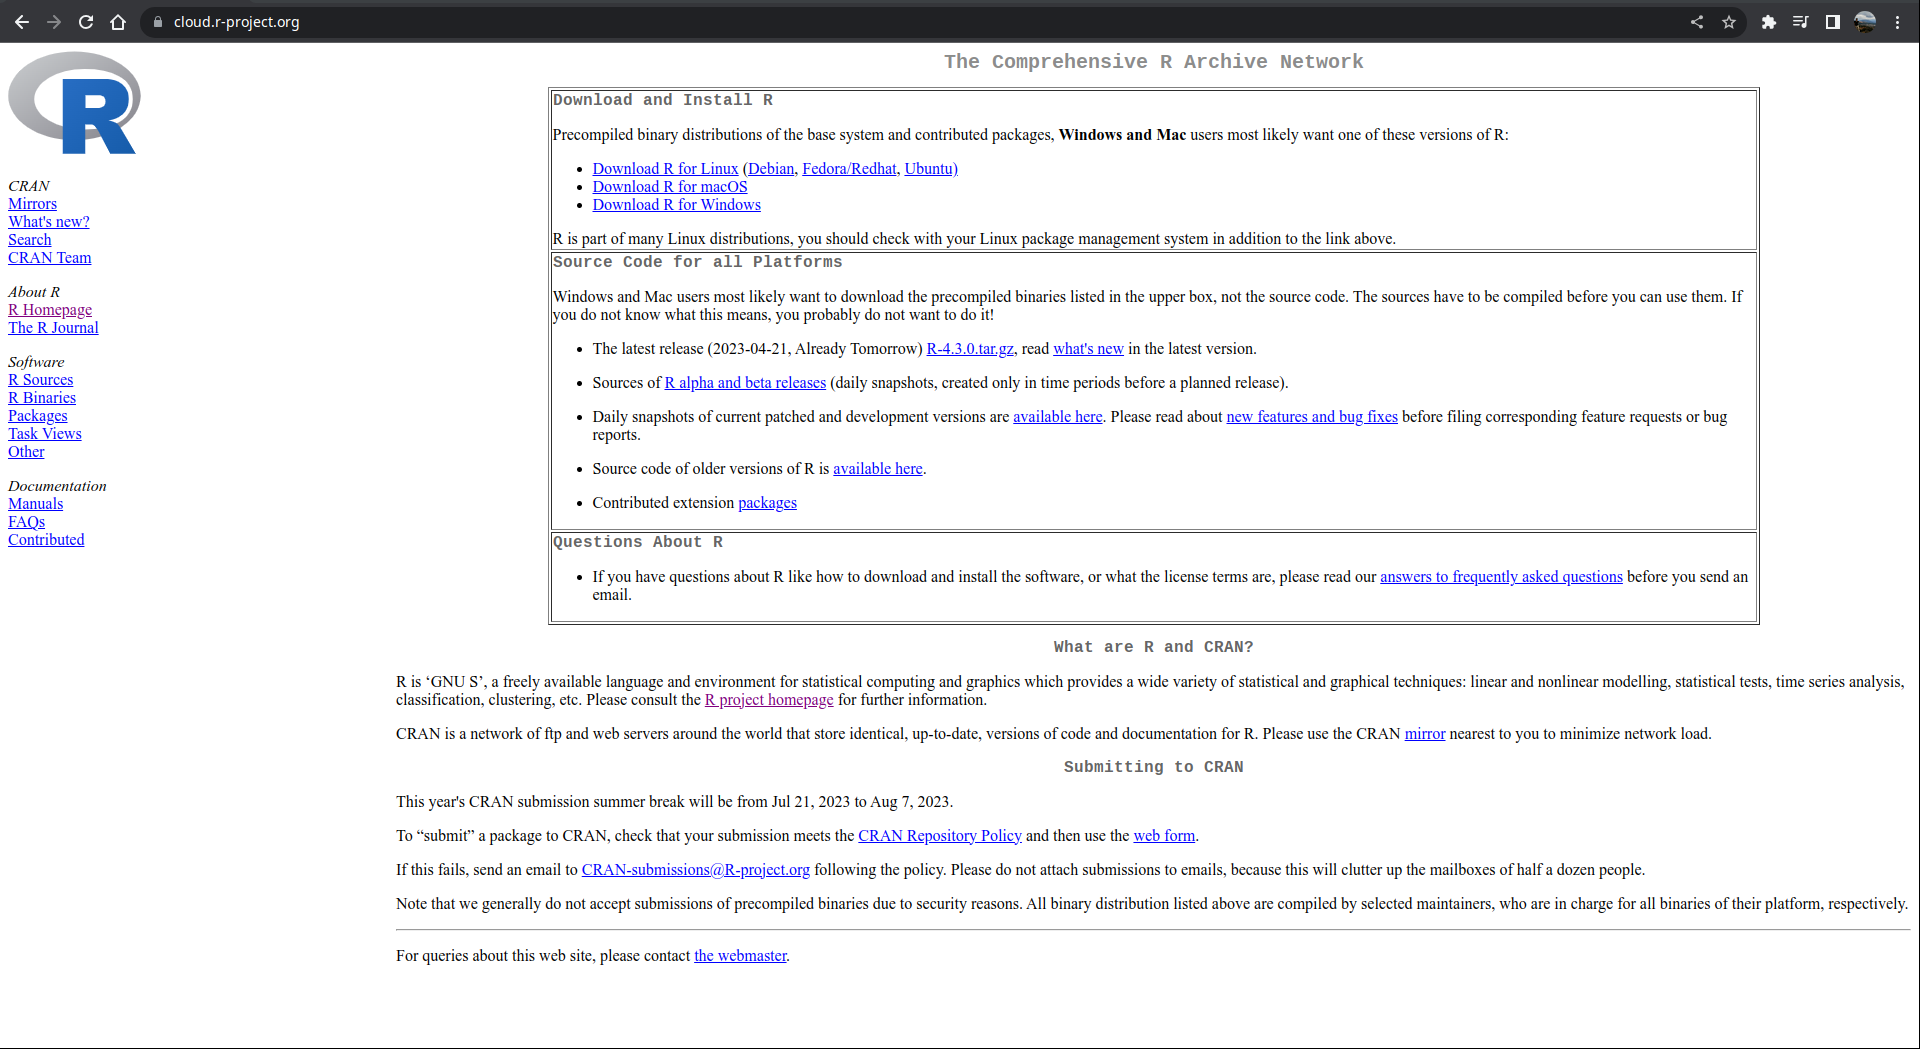
\includegraphics{1-Descargando-Instalando-R-RStudio/images/Screenshot_20230610_222900.png}

\hypertarget{paso-2.-instalar-r-en-ubuntu-linux}{%
\section{Paso 2. Instalar R en Ubuntu
Linux}\label{paso-2.-instalar-r-en-ubuntu-linux}}

Los paquetes para la versión actual de R 4.2 están disponibles para la
mayoría de las versiones estables de Ubuntu Desktop. Sin embargo, solo
la última versión de Soporte a Largo Plazo (LTS) cuenta con soporte
completo. A partir del 2 de mayo de 2022, las versiones compatibles son:

\begin{itemize}
\tightlist
\item
  Jammy Jellyfish (22.04, solo amd64)
\item
  Impish Indri (21.10, solo amd64)
\item
  Focal Fossa (20.04; LTS y solo amd64)
\item
  Bionic Beaver (18.04; LTS)
\item
  Xenial Xerus (16.04; LTS)
\end{itemize}

Ejecuta estas líneas (si eres \texttt{root}, omite \texttt{sudo}) para
informar a Ubuntu sobre los binarios de R en CRAN.

\begin{Shaded}
\begin{Highlighting}[]
\CommentTok{\# Actualizar índices}
\FunctionTok{sudo}\NormalTok{ apt update }\AttributeTok{{-}qq}
\CommentTok{\# Instalar dos paquetes auxiliares necesarios}
\FunctionTok{sudo}\NormalTok{ apt install }\AttributeTok{{-}{-}no{-}install{-}recommends}\NormalTok{ software{-}properties{-}common dirmngr}
\CommentTok{\# Agregar la clave de firma (de Michael Rutter) para estos repositorios}
\CommentTok{\# Para verificar la clave, ejecuta: gpg {-}{-}show{-}keys /etc/apt/trusted.gpg.d/cran\_ubuntu\_key.asc}
\CommentTok{\# Huella digital: E298A3A825C0D65DFD57CBB651716619E084DAB9}
\FunctionTok{wget} \AttributeTok{{-}qO{-}}\NormalTok{ https://cloud.r{-}project.org/bin/linux/ubuntu/marutter\_pubkey.asc }\KeywordTok{|} \FunctionTok{sudo}\NormalTok{ tee }\AttributeTok{{-}a}\NormalTok{ /etc/apt/trusted.gpg.d/cran\_ubuntu\_key.asc}
\CommentTok{\# Agregar el repositorio de R 4.0 de CRAN {-}{-} ajustar \textquotesingle{}focal\textquotesingle{} a \textquotesingle{}groovy\textquotesingle{} o \textquotesingle{}bionic\textquotesingle{} según sea necesario}
\FunctionTok{sudo}\NormalTok{ add{-}apt{-}repository }\StringTok{"deb https://cloud.r{-}project.org/bin/linux/ubuntu }\VariableTok{$(}\ExtensionTok{lsb\_release} \AttributeTok{{-}cs}\VariableTok{)}\StringTok{{-}cran40/"}
\end{Highlighting}
\end{Shaded}

Aquí utilizamos \texttt{lsb\_release\ -cs} para acceder a la versión de
Ubuntu que estás utilizando: ``jammy'', ``impish'', ``focal'',
``bionic'', \ldots{}

Luego, ejecuta

\begin{Shaded}
\begin{Highlighting}[]
\FunctionTok{sudo}\NormalTok{ apt install }\AttributeTok{{-}{-}no{-}install{-}recommends}\NormalTok{ r{-}base}
\end{Highlighting}
\end{Shaded}

\hypertarget{obtuxe9n-muxe1s-de-5000-paquetes-de-cran}{%
\section{Obtén más de 5000 paquetes de
CRAN}\label{obtuxe9n-muxe1s-de-5000-paquetes-de-cran}}

Ejecuta este comando (como \texttt{root} o agregando \texttt{sudo} como
prefijo) para agregar el repositorio actual de R 4.0 o posterior
`c2d4u':

\begin{Shaded}
\begin{Highlighting}[]
\FunctionTok{sudo}\NormalTok{ add{-}apt{-}repository ppa:c2d4u.team/c2d4u4.0+}
\end{Highlighting}
\end{Shaded}

para agregar el ID de clave de este repositorio, agregar el repositorio
y actualizar el índice. Ahora puedes hacer
\texttt{apt\ install\ -\/-no-install-recommends\ r-cran-rstan} o
\texttt{apt\ install\ -\/-no-install-recommends\ r-cran-tidyverse}
(nuevamente como usuario \texttt{root} o a través de \texttt{sudo}).

\hypertarget{paso-3.-descargar-rstudio-en-ubuntu-linux}{%
\section{Paso 3. Descargar RStudio en Ubuntu
Linux}\label{paso-3.-descargar-rstudio-en-ubuntu-linux}}

Puedes descargar la última versión de RStudio desde su sitio web
oficial:
\href{https://www.rstudio.com/products/rstudio/download/}{Enlace de
descarga de RStudio}

\begin{quote}
RStudio RStudio es un entorno de desarrollo integrado (IDE) muy popular
para trabajar con R. Proporciona una interfaz gráfica intuitiva y muchas
herramientas útiles para la programación en R.
\end{quote}

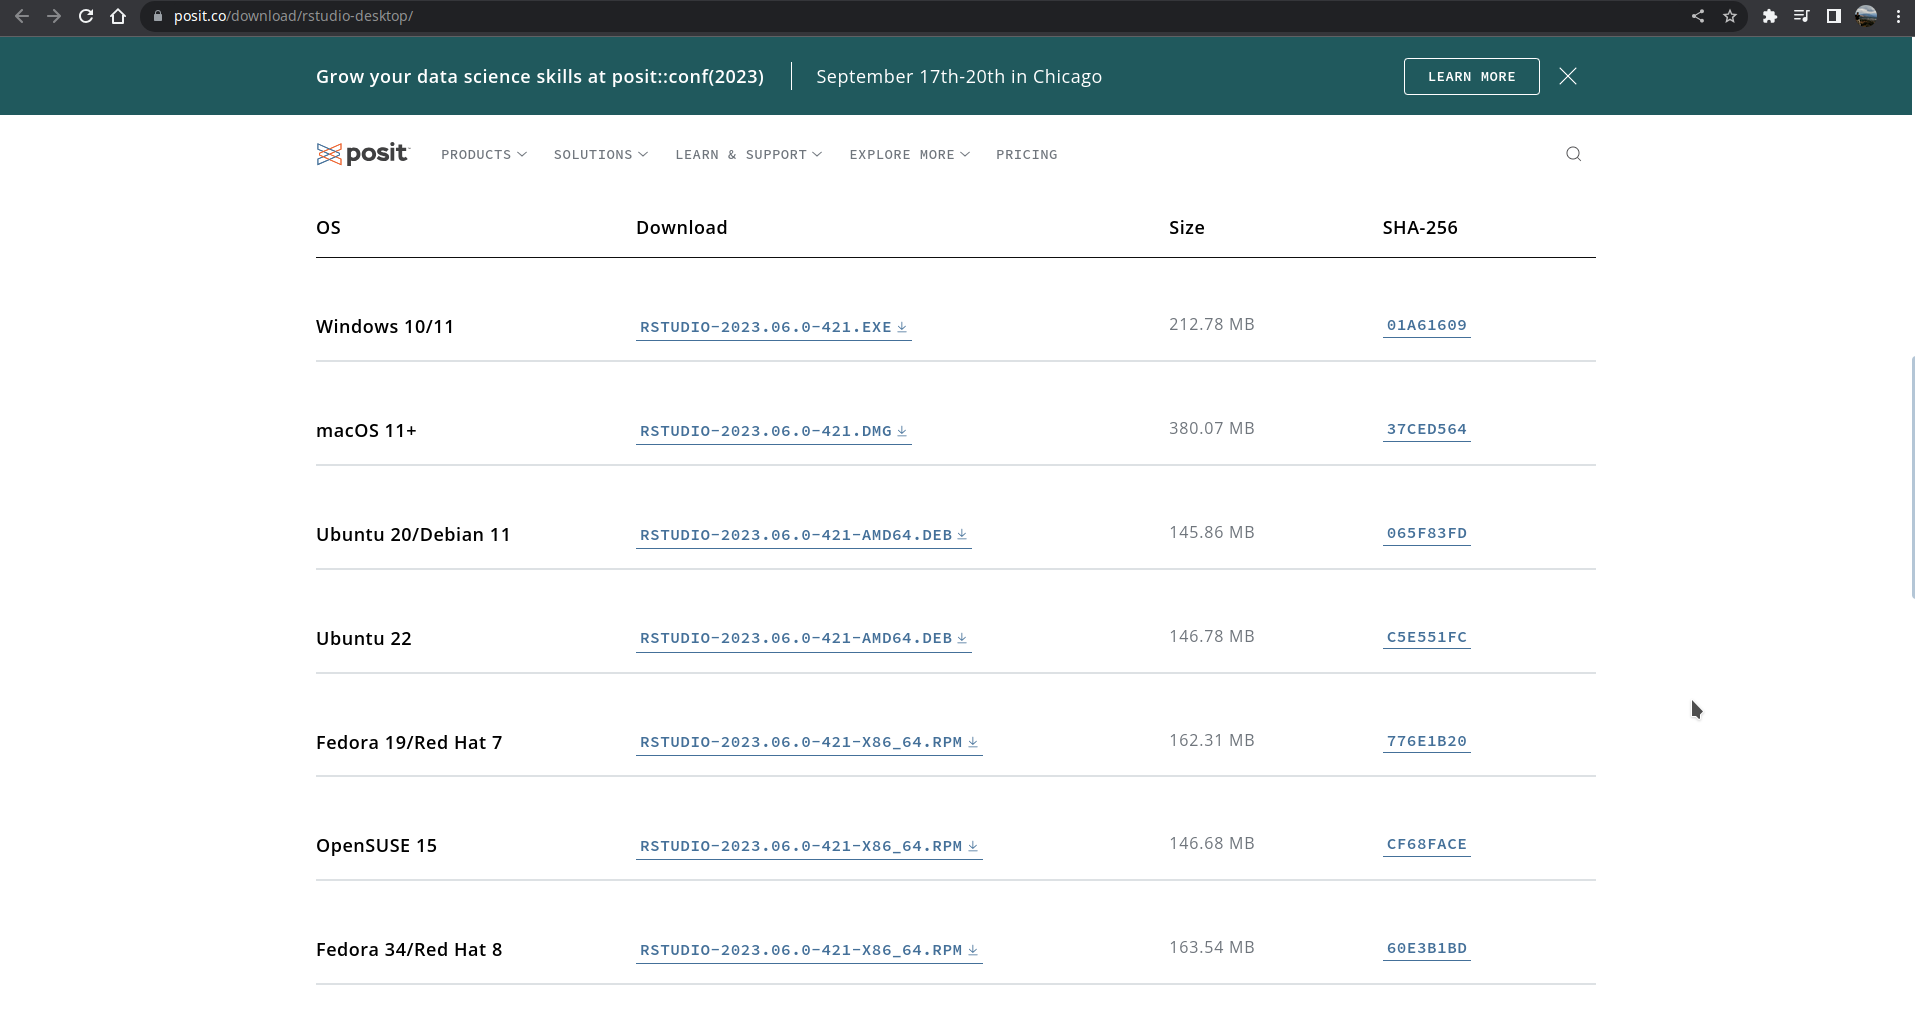
\includegraphics{1-Descargando-Instalando-R-RStudio/images/Screenshot_20230610_224818.png}

\hypertarget{paso-4.-instalar-rstudio-en-ubuntu-linux}{%
\section{Paso 4. Instalar RStudio en Ubuntu
Linux}\label{paso-4.-instalar-rstudio-en-ubuntu-linux}}

\hypertarget{instalar-dependencias}{%
\subsection{Instalar dependencias}\label{instalar-dependencias}}

Antes de instalar RStudio, es posible que debas instalar algunas
dependencias en tu sistema. Abre la terminal y ejecuta los siguientes
comandos para instalar las dependencias requeridas:

\begin{Shaded}
\begin{Highlighting}[]
\FunctionTok{sudo}\NormalTok{ apt update}
\FunctionTok{sudo}\NormalTok{ apt install gdebi{-}core}
\end{Highlighting}
\end{Shaded}

Estos comandos actualizarán los repositorios de paquetes y luego
instalarán \texttt{gdebi-core}, una utilidad necesaria para instalar
paquetes \texttt{.deb} de forma sencilla y para resolver dependencias
automáticamente.

\hypertarget{instalar-rstudio}{%
\subsection{Instalar RStudio}\label{instalar-rstudio}}

Una vez que hayas descargado el archivo de instalación de RStudio y
hayas instalado las dependencias necesarias, puedes proceder con la
instalación. Ve al directorio donde descargaste el archivo de
instalación y ejecuta el siguiente comando en la terminal:

\begin{Shaded}
\begin{Highlighting}[]
\FunctionTok{sudo}\NormalTok{ gdebi }\OperatorTok{\textless{}}\NormalTok{nombre\_del\_archivo\_de\_instalación}\OperatorTok{\textgreater{}}\NormalTok{.deb}
\end{Highlighting}
\end{Shaded}

Reemplaza
\texttt{\textless{}nombre\_del\_archivo\_de\_instalación\textgreater{}}
con el nombre real del archivo de instalación descargado.

El comando \texttt{gdebi} instalará RStudio y resolverá automáticamente
las dependencias necesarias.

\hypertarget{paso-5.-iniciar-rstudio}{%
\section{Paso 5. Iniciar RStudio}\label{paso-5.-iniciar-rstudio}}

Una vez completada la instalación, puedes iniciar RStudio desde el menú
de aplicaciones de Ubuntu o ejecutando el siguiente comando en la
terminal:

\begin{Shaded}
\begin{Highlighting}[]
\ExtensionTok{rstudio}
\end{Highlighting}
\end{Shaded}

RStudio se abrirá en una ventana separada, lo que te permitirá comenzar
a trabajar con R y aprovechar todas las funciones y características que
ofrece el IDE.

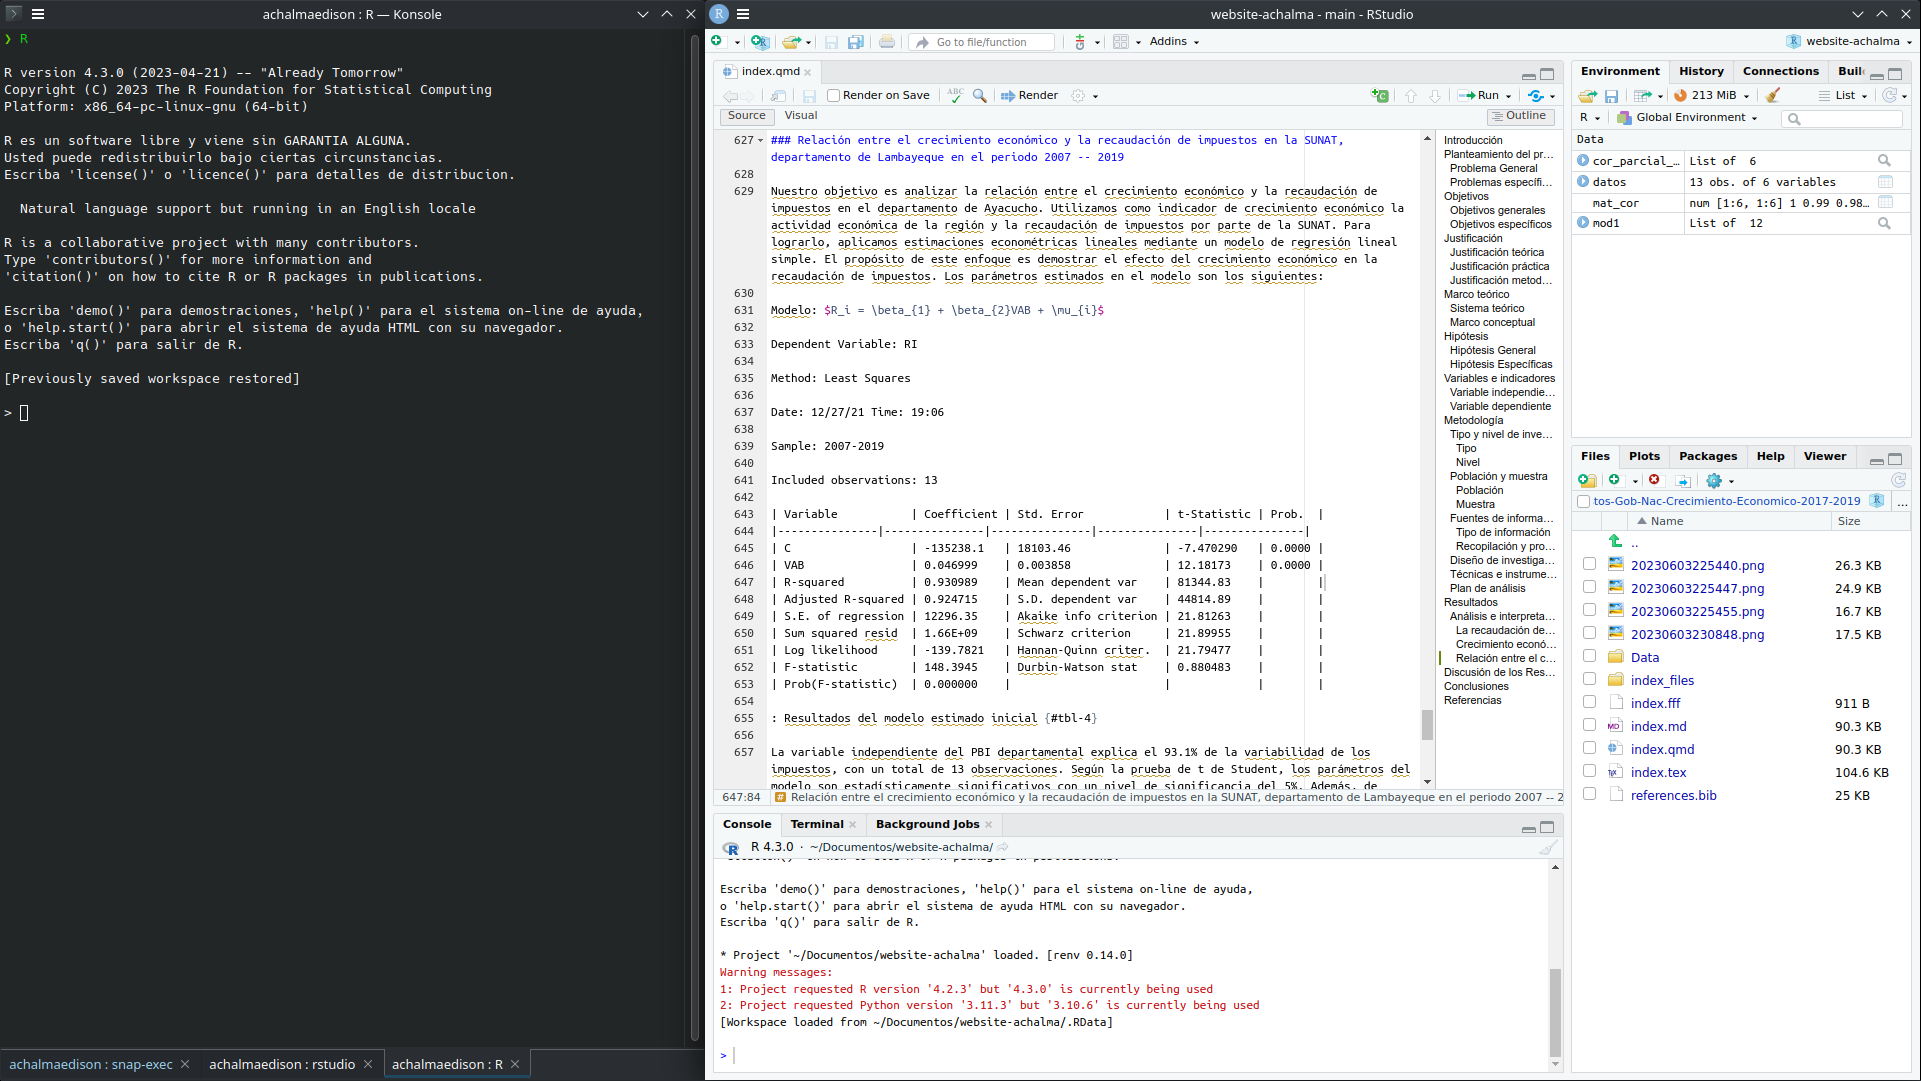
\includegraphics{1-Descargando-Instalando-R-RStudio/images/Screenshot_20230610_231407.png}

\hypertarget{quxfae-nos-ofrece-rstudio}{%
\chapter{¿Qúe nos ofrece RStudio?}\label{quxfae-nos-ofrece-rstudio}}

\hypertarget{beneficios-del-software-rstudio}{%
\section{Beneficios del software
RStudio}\label{beneficios-del-software-rstudio}}

RStudio es una herramienta poderosa que brinda numerosas ventajas para
los usuarios. A continuación, destacamos algunas de las funcionalidades
que ofrece:

\begin{enumerate}
\def\labelenumi{\arabic{enumi}.}
\item
  \textbf{Potente editor de código:} RStudio proporciona un entorno de
  desarrollo integrado (IDE) que cuenta con un editor de código robusto.
  Este editor permite escribir, editar y ejecutar código de manera
  eficiente, lo que facilita el trabajo con el lenguaje de programación
  R.
\item
  \textbf{Gestión del espacio de trabajo:} RStudio ofrece
  características avanzadas para el manejo del espacio de trabajo.
  Puedes explorar y administrar fácilmente los objetos, variables y
  funciones utilizados en tu sesión de R, lo que facilita el seguimiento
  y la organización de tus datos y resultados.
\item
  \textbf{Depuración y resaltado de sintaxis:} La función de depuración
  de RStudio te permite identificar y corregir errores en tu código de
  manera eficiente. Además, el resaltado de sintaxis te ayuda a
  visualizar y comprender mejor la estructura de tu código, lo que
  facilita su lectura y mantenimiento.
\item
  \textbf{Autocompletado inteligente:} RStudio ofrece una función de
  autocompletado inteligente, que te sugiere opciones de código a medida
  que escribes. Esto acelera el proceso de codificación al proporcionar
  sugerencias contextuales y facilitar la escritura correcta de las
  funciones y objetos de R.
\item
  \textbf{Interoperabilidad con otros software y plataformas:} RStudio
  es compatible con una amplia gama de herramientas y plataformas.
  Puedes integrar fácilmente tus análisis en flujos de trabajo
  existentes, colaborar con otros profesionales y compartir tus
  resultados en diferentes formatos, como informes, gráficos
  interactivos o aplicaciones web.
\end{enumerate}

\begin{figure}

{\centering 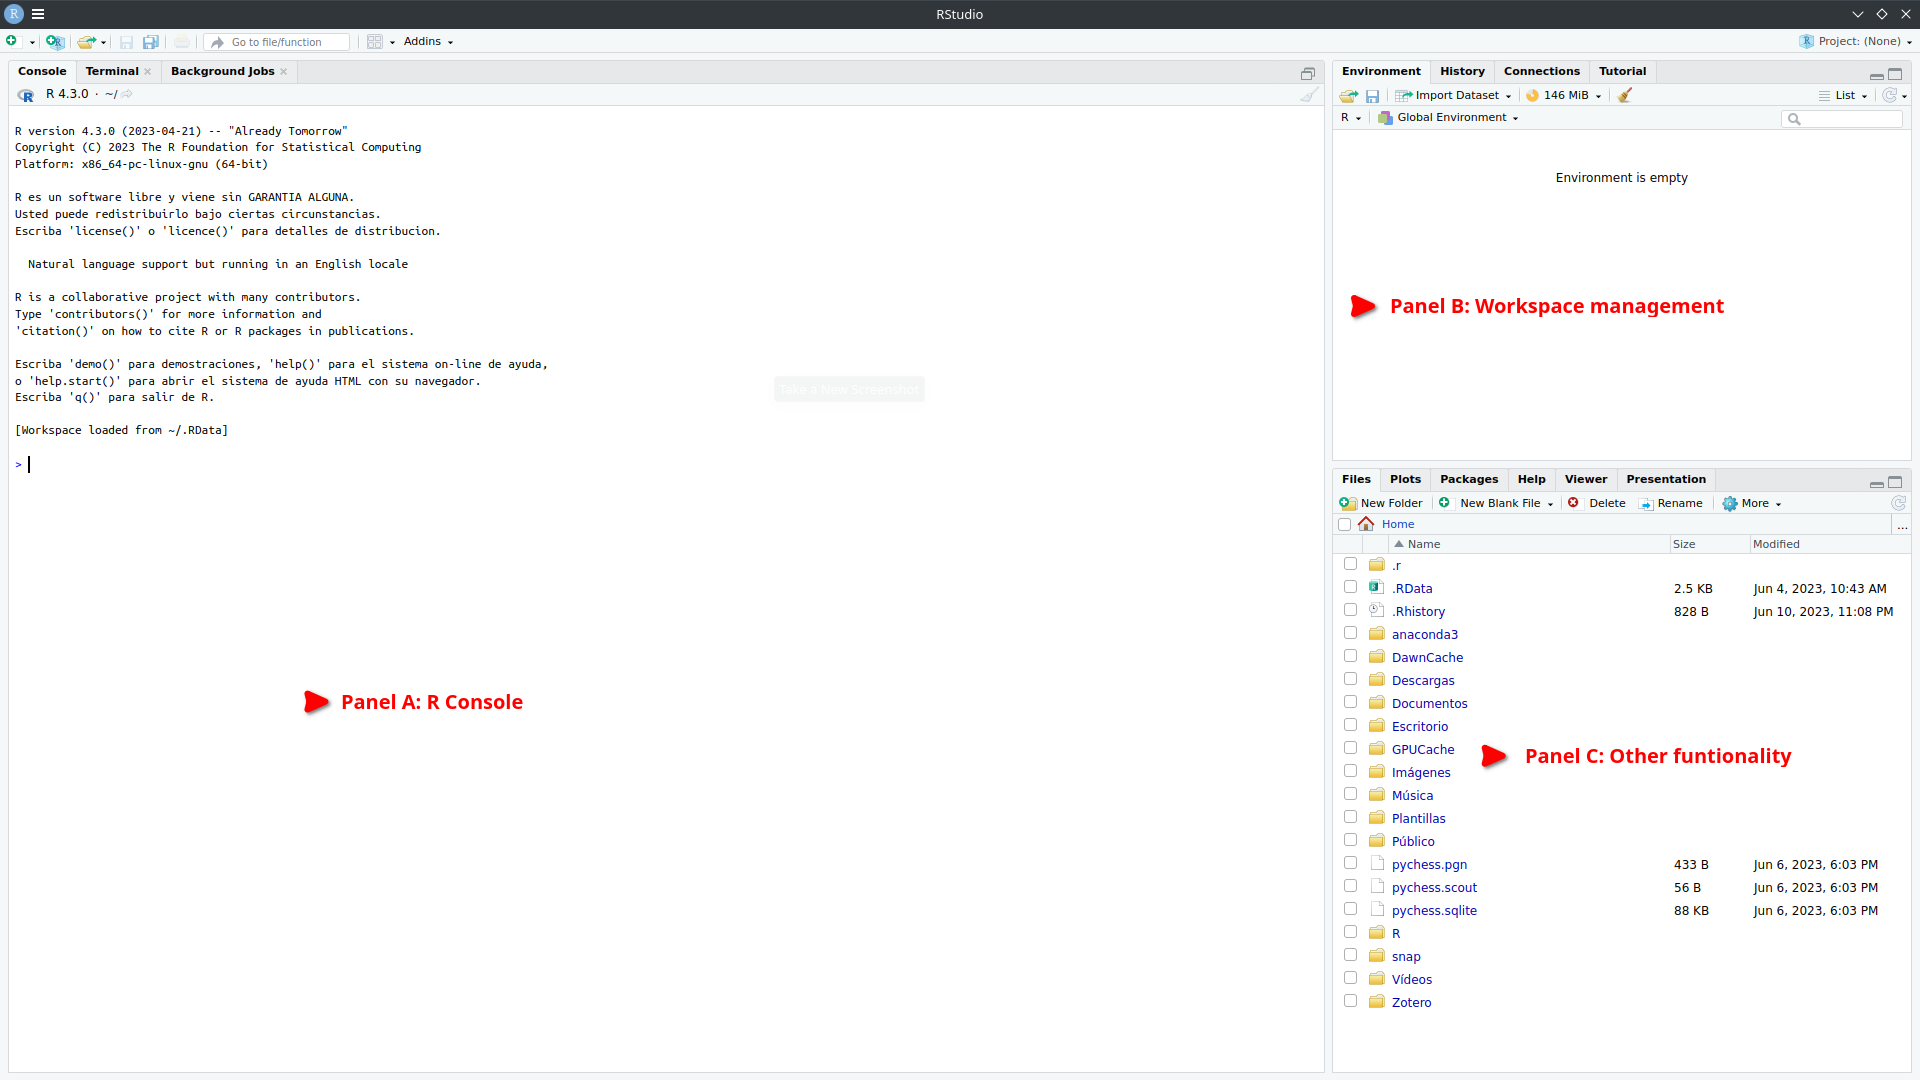
\includegraphics{2-Que-Ofrece-RStudio/images/Screenshot_20230610_233058.png}

}

\caption{Interfaz de RStudio: Una poderosa herramienta para el
desarrollo en R}

\end{figure}

\hypertarget{archivos-de-script-en-r-.r}{%
\section{Archivos de Script en R
(.R)}\label{archivos-de-script-en-r-.r}}

En el mundo del análisis de datos y programación en R, los archivos de
script (.R) desempeñan un papel fundamental. Estos archivos contienen la
secuencia de comandos necesaria para realizar análisis y manipulación de
datos de manera sistemática y reproducible.

\hypertarget{ventajas-de-utilizar-archivos-de-script-en-r}{%
\subsection{Ventajas de utilizar archivos de script en
R:}\label{ventajas-de-utilizar-archivos-de-script-en-r}}

\begin{enumerate}
\def\labelenumi{\arabic{enumi}.}
\item
  \textbf{Documentación de tareas}: Al escribir nuestros comandos en un
  archivo de script, estamos creando una documentación detallada de los
  pasos y procesos utilizados en nuestro análisis. Esto facilita la
  comprensión y revisión de nuestro trabajo, tanto para nosotros mismos
  como para otros colaboradores.
\item
  \textbf{Automatización de tareas repetitivas}: Los archivos de script
  permiten automatizar tareas que se repiten con frecuencia. Podemos
  definir una serie de comandos en el archivo y ejecutarlos de forma
  rápida y eficiente cada vez que sea necesario. Esto ahorra tiempo y
  reduce la posibilidad de errores.
\item
  \textbf{Evaluación de cambios}: Al tener nuestros comandos en un
  archivo de script, podemos realizar modificaciones y ajustes en el
  análisis de manera más ágil. Podemos realizar pruebas y evaluaciones
  de los cambios sin necesidad de volver a escribir todo el código desde
  cero. Esto nos brinda flexibilidad y nos permite iterar y mejorar
  nuestro análisis de manera más eficiente.
\end{enumerate}

\hypertarget{creando-y-ejecutando-un-script-en-rstudio}{%
\subsection{Creando y Ejecutando un Script en
RStudio}\label{creando-y-ejecutando-un-script-en-rstudio}}

Los scripts nos permiten escribir y ejecutar una serie de comandos de
manera secuencial, lo que facilita la automatización y reproducción de
tareas en nuestros análisis de datos.

\textbf{Paso 1: Crear un nuevo archivo de script}

En primer lugar, abrimos RStudio y creamos un nuevo archivo de script.
Para hacer esto, seleccionamos ``Archivo'' en la barra de menú, luego
``Nuevo archivo'' y finalmente ``Script R''. Esto abrirá un nuevo editor
de texto donde podemos escribir nuestro código.

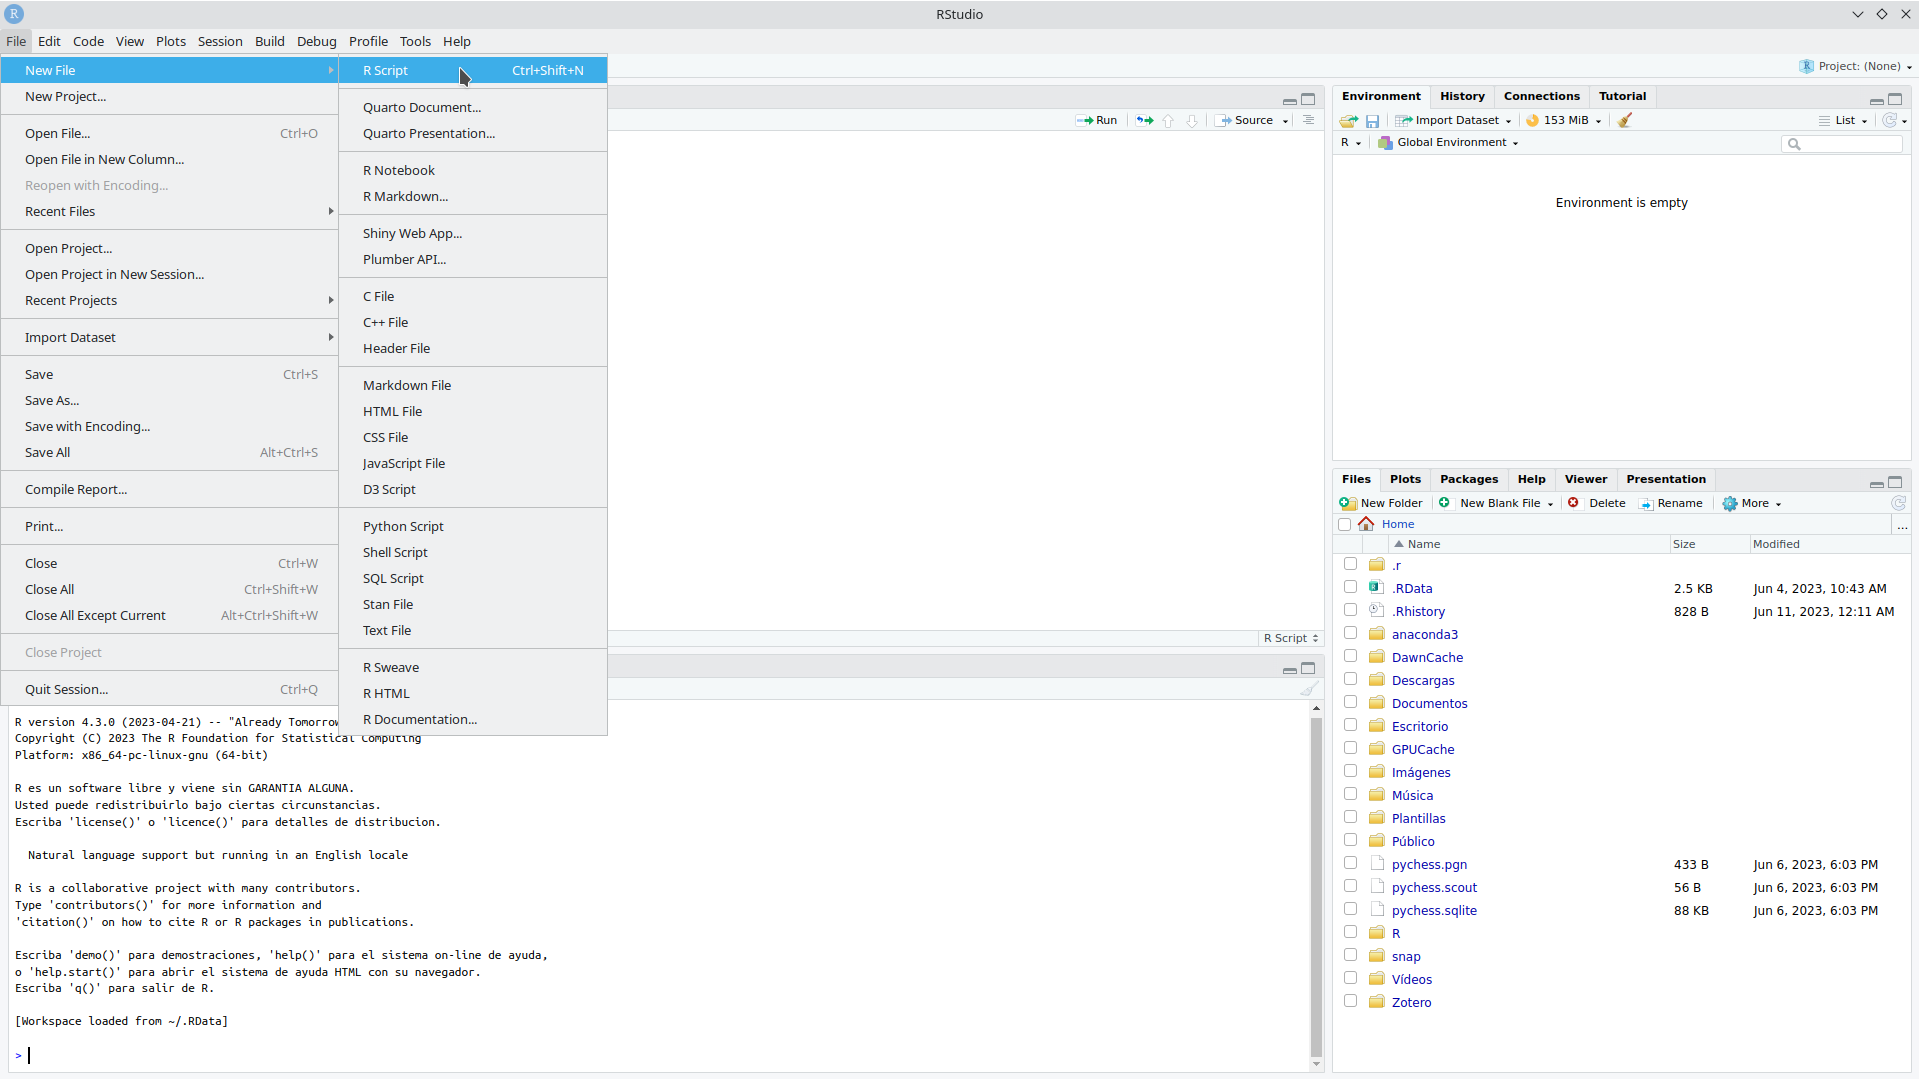
\includegraphics{2-Que-Ofrece-RStudio/images/Screenshot_20230611_001234.png}

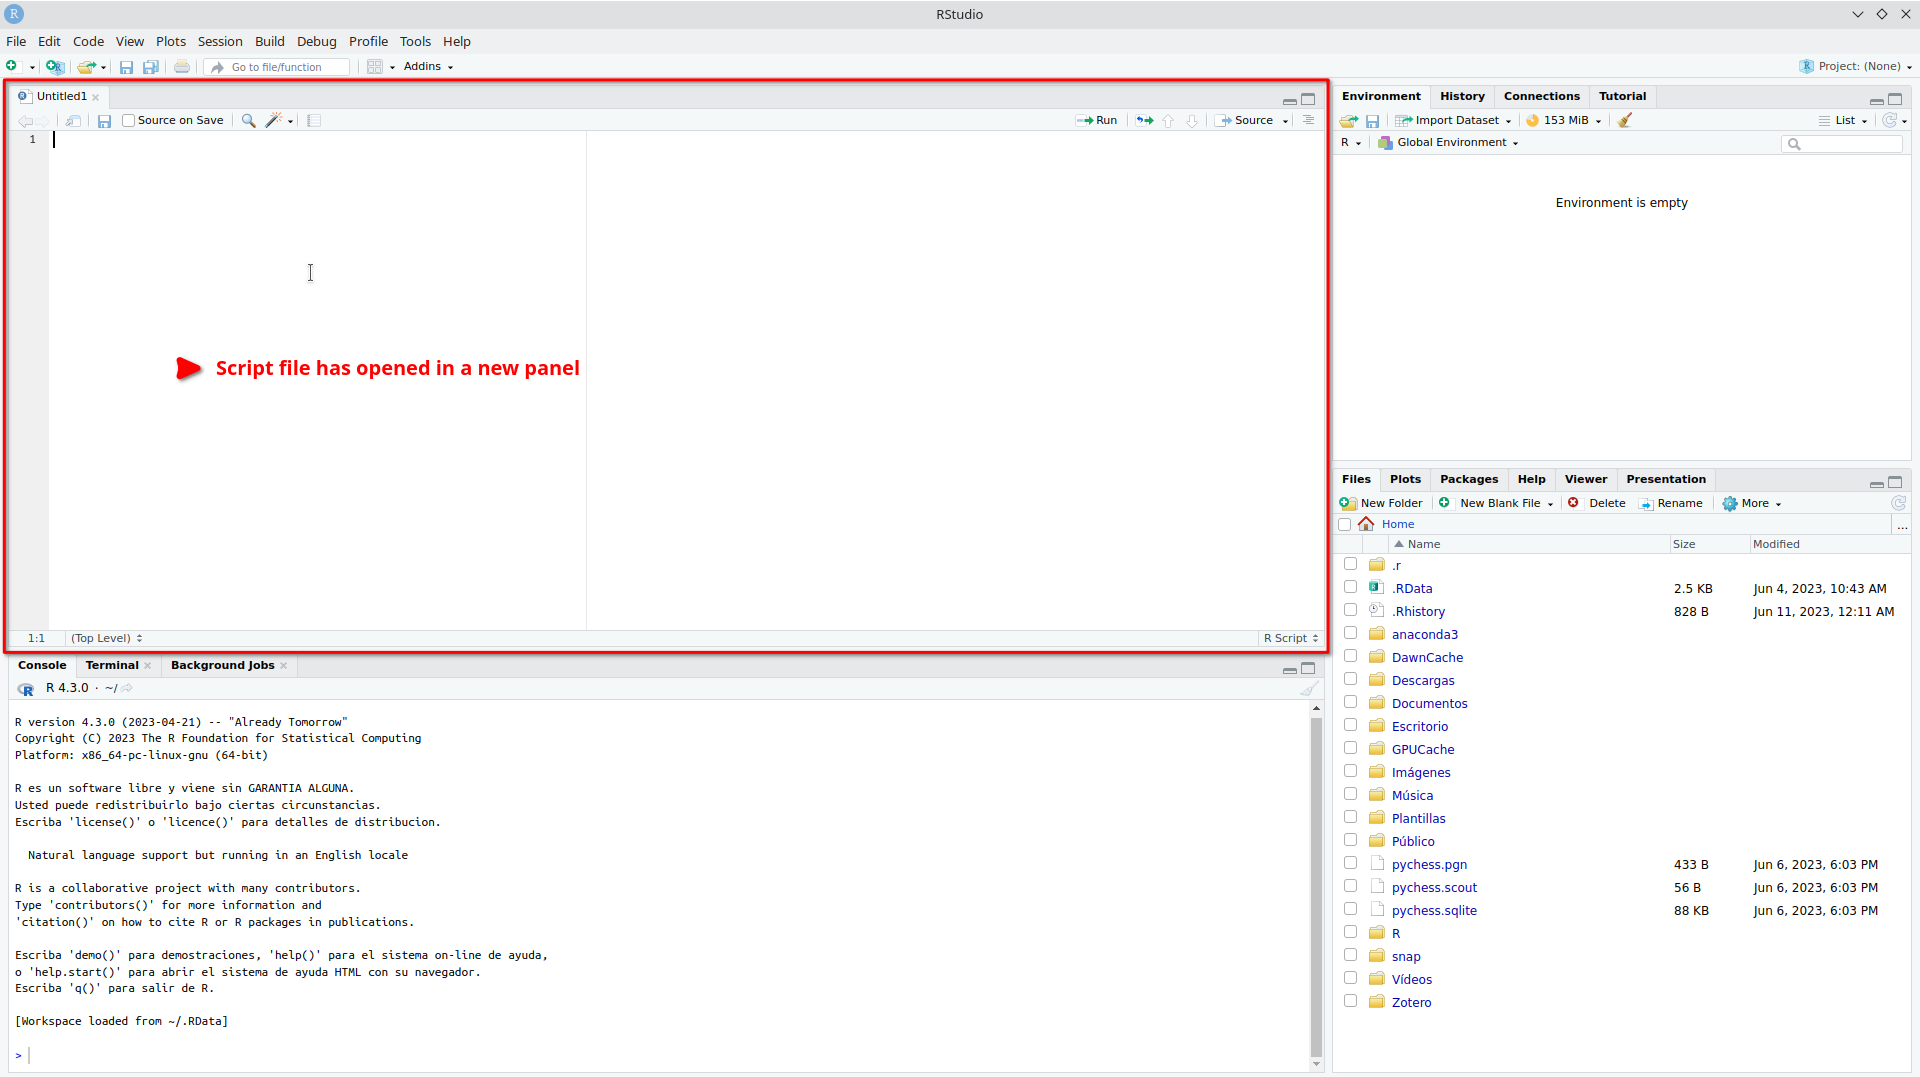
\includegraphics{2-Que-Ofrece-RStudio/images/Screenshot_20230611_001615.png}

\textbf{Paso 2: Escribir el código en el script}

Una vez que tenemos nuestro archivo de script abierto, podemos comenzar
a escribir nuestro código en R. Podemos utilizar cualquier comando o
función de R en el script para realizar análisis de datos, manipulación
de variables, visualización, entre otros. Es importante asegurarse de
que el código esté escrito correctamente y tenga una sintaxis válida.

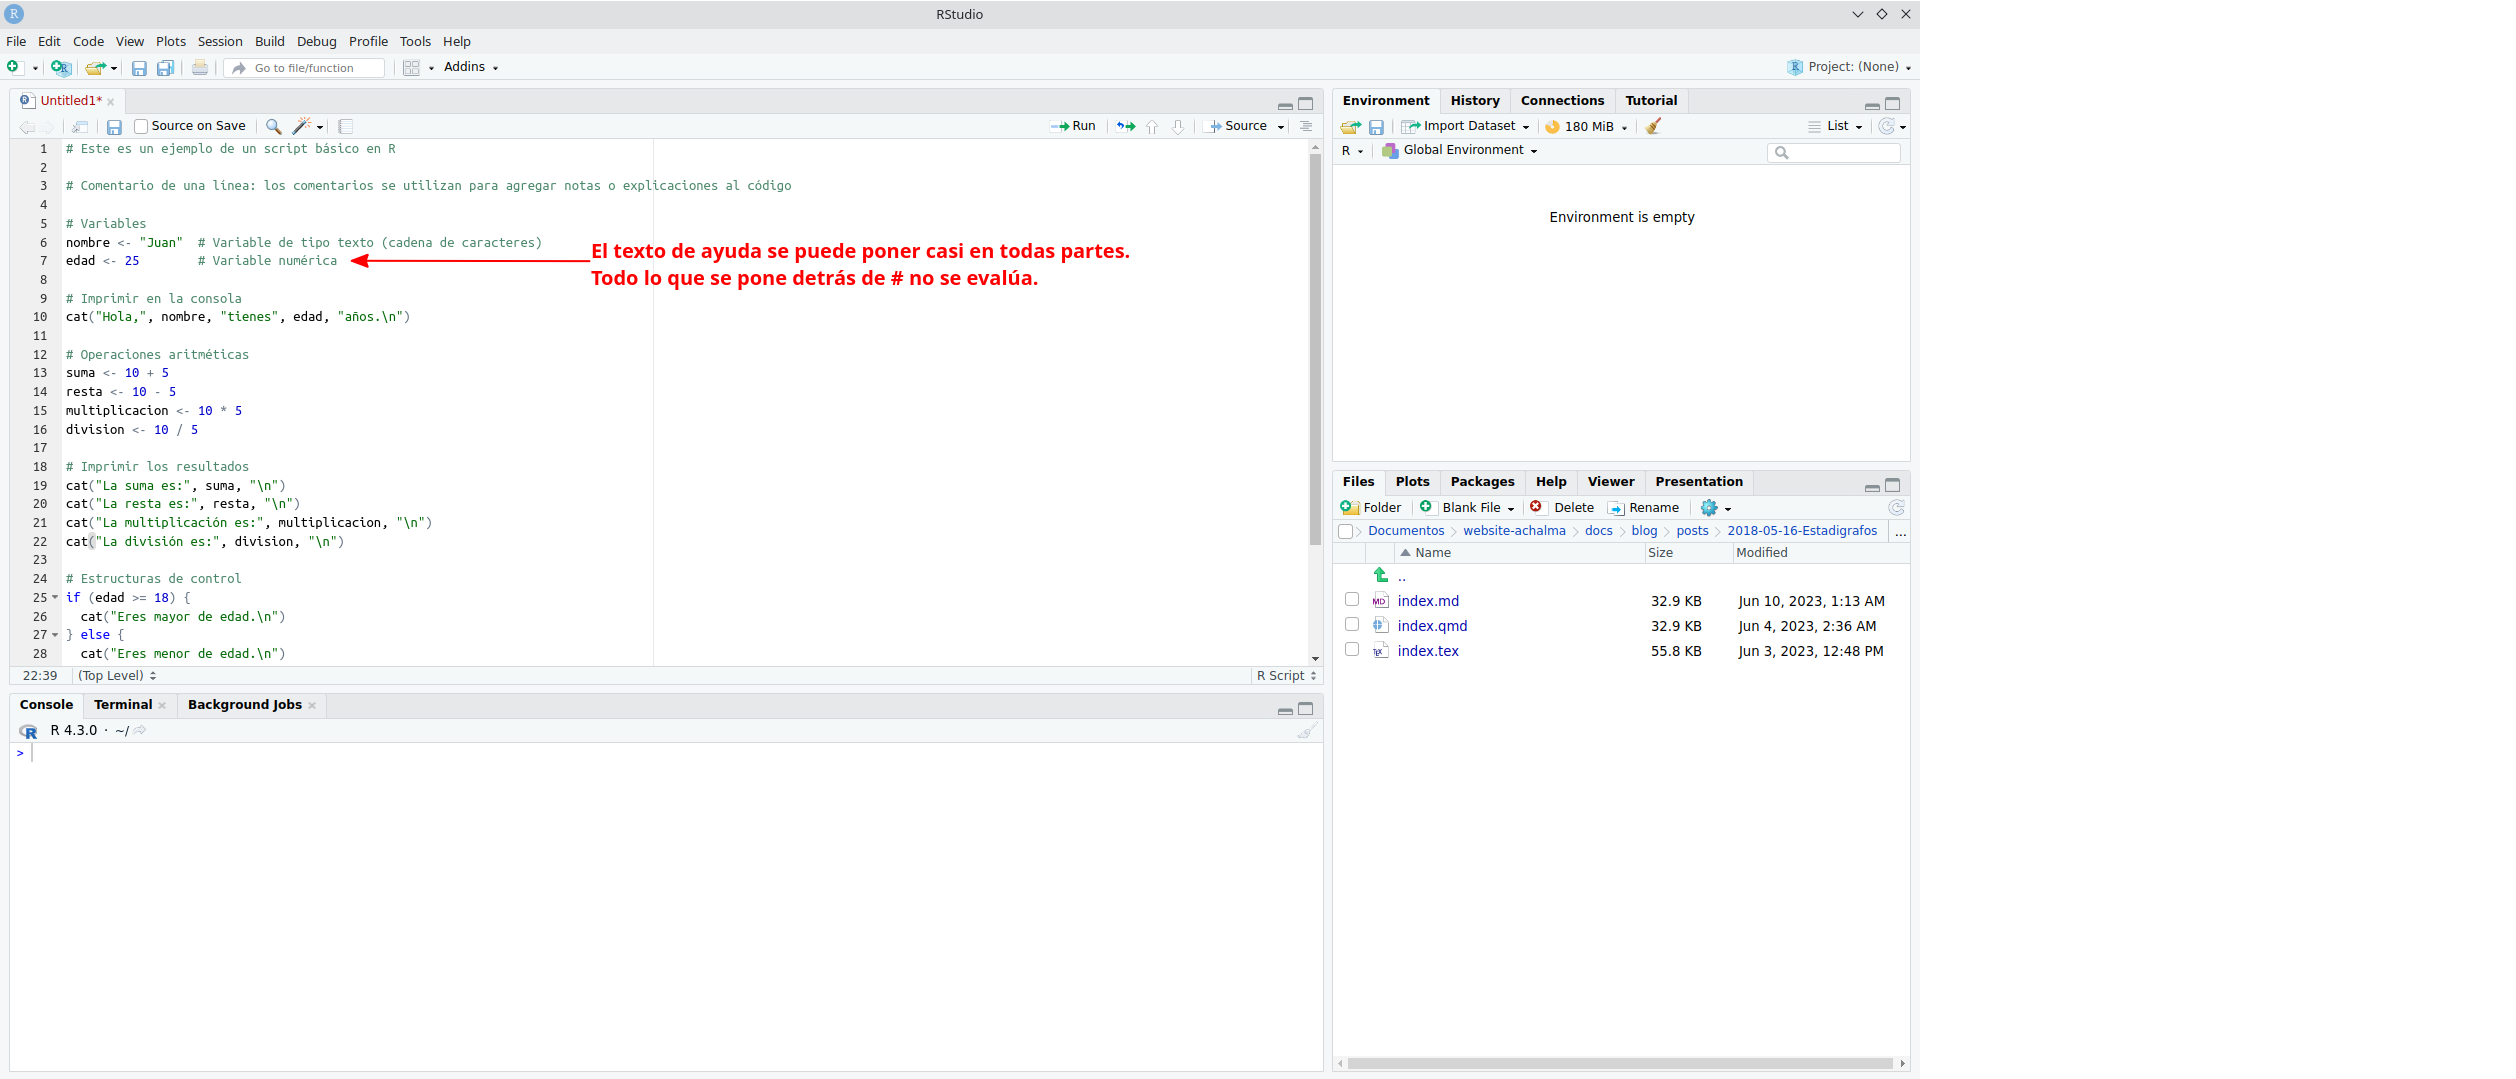
\includegraphics{2-Que-Ofrece-RStudio/images/Screenshot_20230611_004241.png}

\begin{Shaded}
\begin{Highlighting}[]
\CommentTok{\# Este es un ejemplo de un script básico en R}

\CommentTok{\# Comentario de una línea: los comentarios se utilizan para agregar notas o explicaciones al código}

\CommentTok{\# Variables}
\NormalTok{nombre }\OtherTok{\textless{}{-}} \StringTok{"Juan"} \CommentTok{\# Variable de tipo texto (cadena de caracteres)}
\NormalTok{edad }\OtherTok{\textless{}{-}} \DecValTok{25} \CommentTok{\# Variable numérica}

\CommentTok{\# Imprimir en la consola}
\FunctionTok{cat}\NormalTok{(}\StringTok{"Hola,"}\NormalTok{, nombre, }\StringTok{"tienes"}\NormalTok{, edad, }\StringTok{"años.}\SpecialCharTok{\textbackslash{}n}\StringTok{"}\NormalTok{)}

\CommentTok{\# Operaciones aritméticas}
\NormalTok{suma }\OtherTok{\textless{}{-}} \DecValTok{10} \SpecialCharTok{+} \DecValTok{5}
\NormalTok{resta }\OtherTok{\textless{}{-}} \DecValTok{10} \SpecialCharTok{{-}} \DecValTok{5}
\NormalTok{multiplicacion }\OtherTok{\textless{}{-}} \DecValTok{10} \SpecialCharTok{*} \DecValTok{5}
\NormalTok{division }\OtherTok{\textless{}{-}} \DecValTok{10} \SpecialCharTok{/} \DecValTok{5}

\CommentTok{\# Imprimir los resultados}
\FunctionTok{cat}\NormalTok{(}\StringTok{"La suma es:"}\NormalTok{, suma, }\StringTok{"}\SpecialCharTok{\textbackslash{}n}\StringTok{"}\NormalTok{)}
\FunctionTok{cat}\NormalTok{(}\StringTok{"La resta es:"}\NormalTok{, resta, }\StringTok{"}\SpecialCharTok{\textbackslash{}n}\StringTok{"}\NormalTok{)}
\FunctionTok{cat}\NormalTok{(}\StringTok{"La multiplicación es:"}\NormalTok{, multiplicacion, }\StringTok{"}\SpecialCharTok{\textbackslash{}n}\StringTok{"}\NormalTok{)}
\FunctionTok{cat}\NormalTok{(}\StringTok{"La división es:"}\NormalTok{, division, }\StringTok{"}\SpecialCharTok{\textbackslash{}n}\StringTok{"}\NormalTok{)}
\end{Highlighting}
\end{Shaded}

\textbf{Paso 3: Ejecutar el script}

Una vez que hemos escrito nuestro código en el archivo de script,
podemos ejecutarlo para obtener los resultados deseados. Para hacer
esto, podemos utilizar el atajo de teclado ``Ctrl + Enter'' o
simplemente hacer clic en el botón ``Ejecutar'' en la parte superior del
editor de texto.

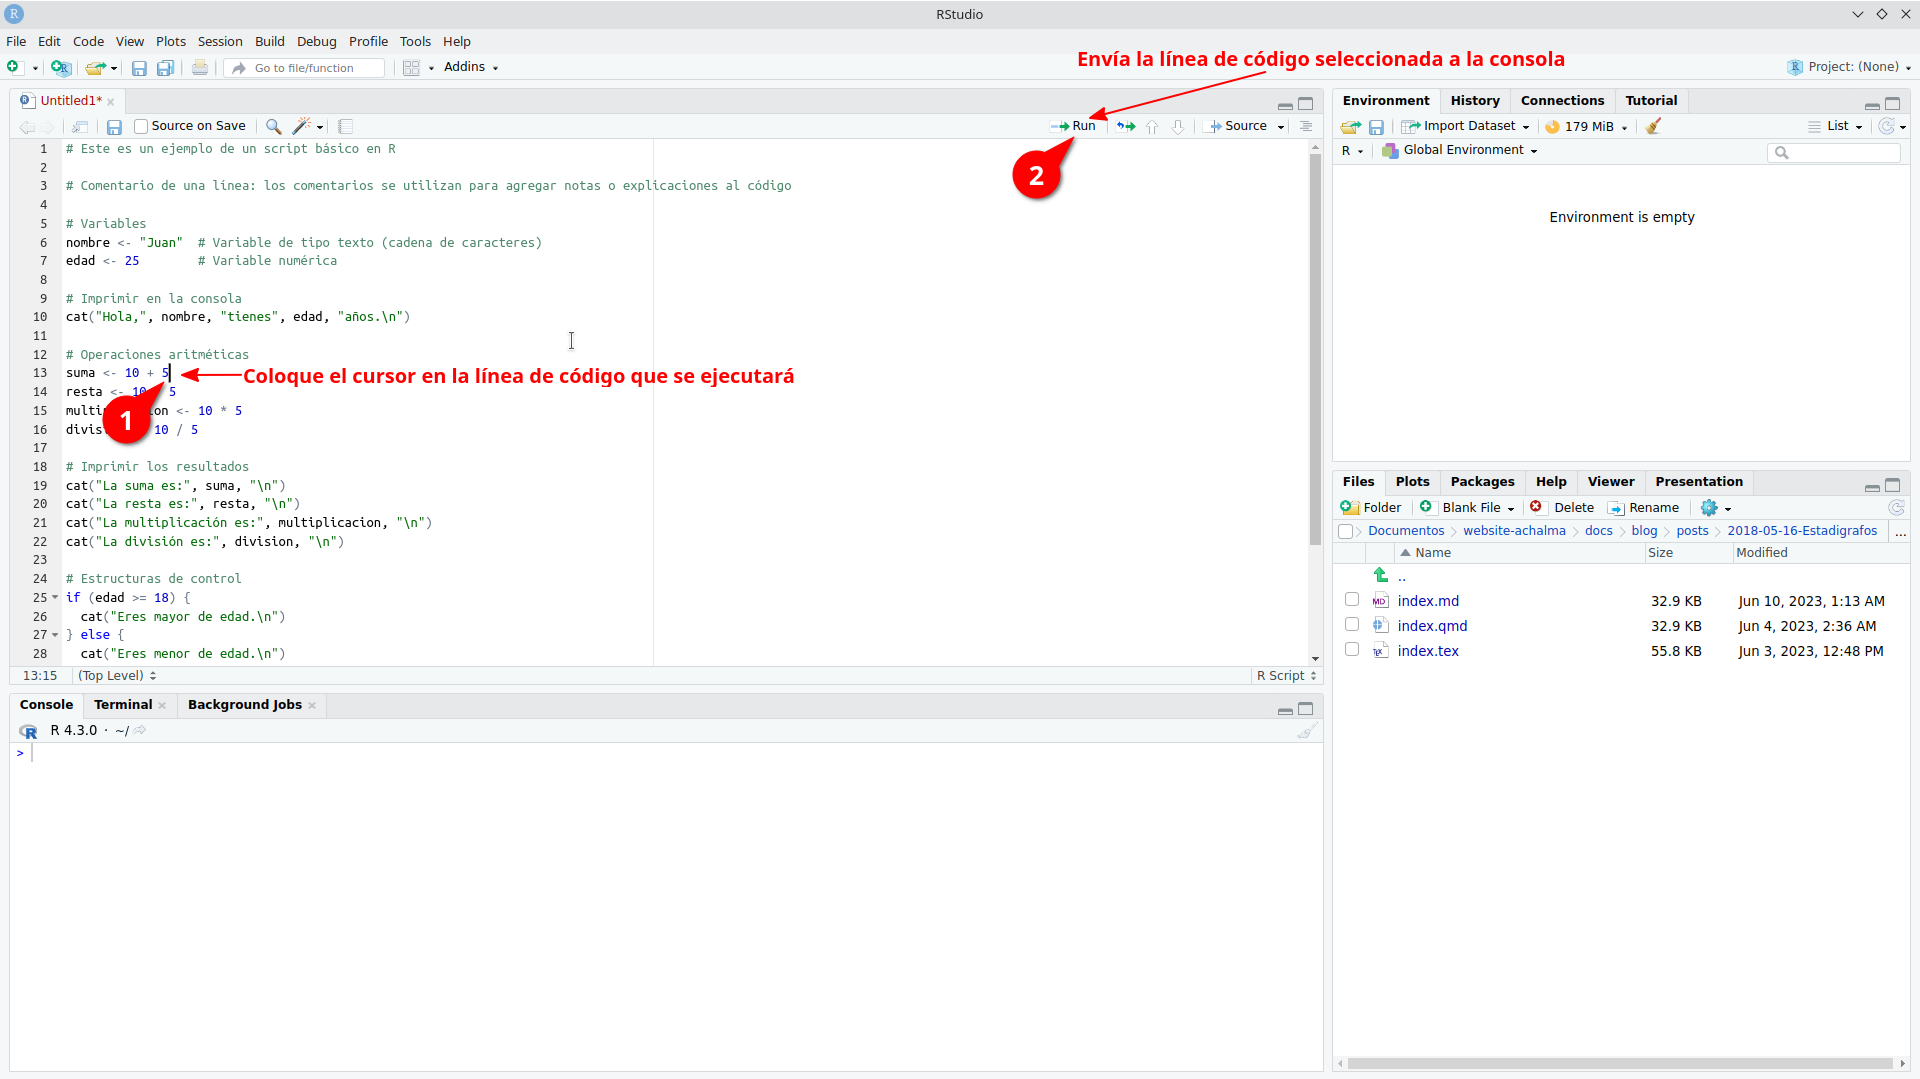
\includegraphics{2-Que-Ofrece-RStudio/images/Screenshot_20230611_005354.png}

RStudio ejecutará el código línea por línea y mostrará los resultados en
la consola.

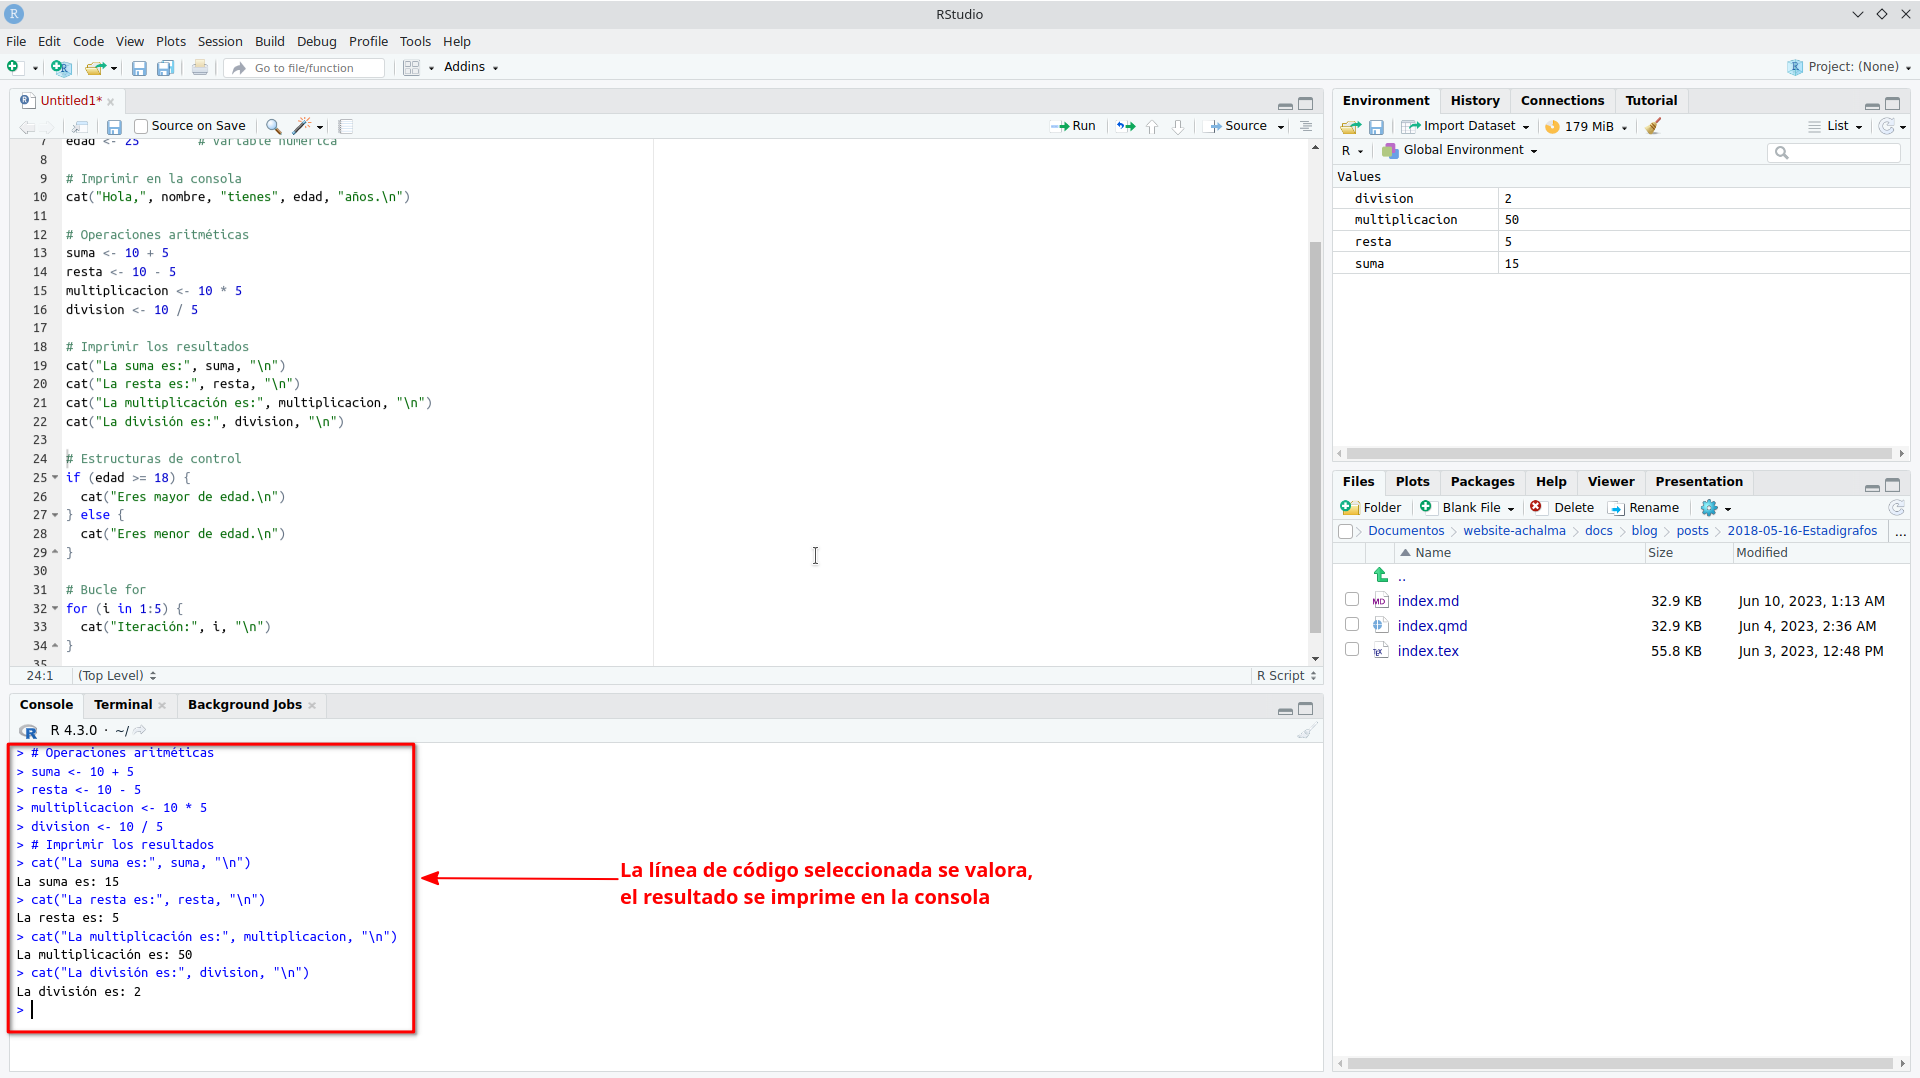
\includegraphics{2-Que-Ofrece-RStudio/images/Screenshot_20230611_010256.png}

\textbf{Paso 4: Guardar el script}

Es importante guardar regularmente nuestro script para evitar perder
nuestro trabajo. Para guardar el archivo de script, seleccionamos
``Archivo'' en la barra de menú y luego ``Guardar'' o ``Guardar como''.

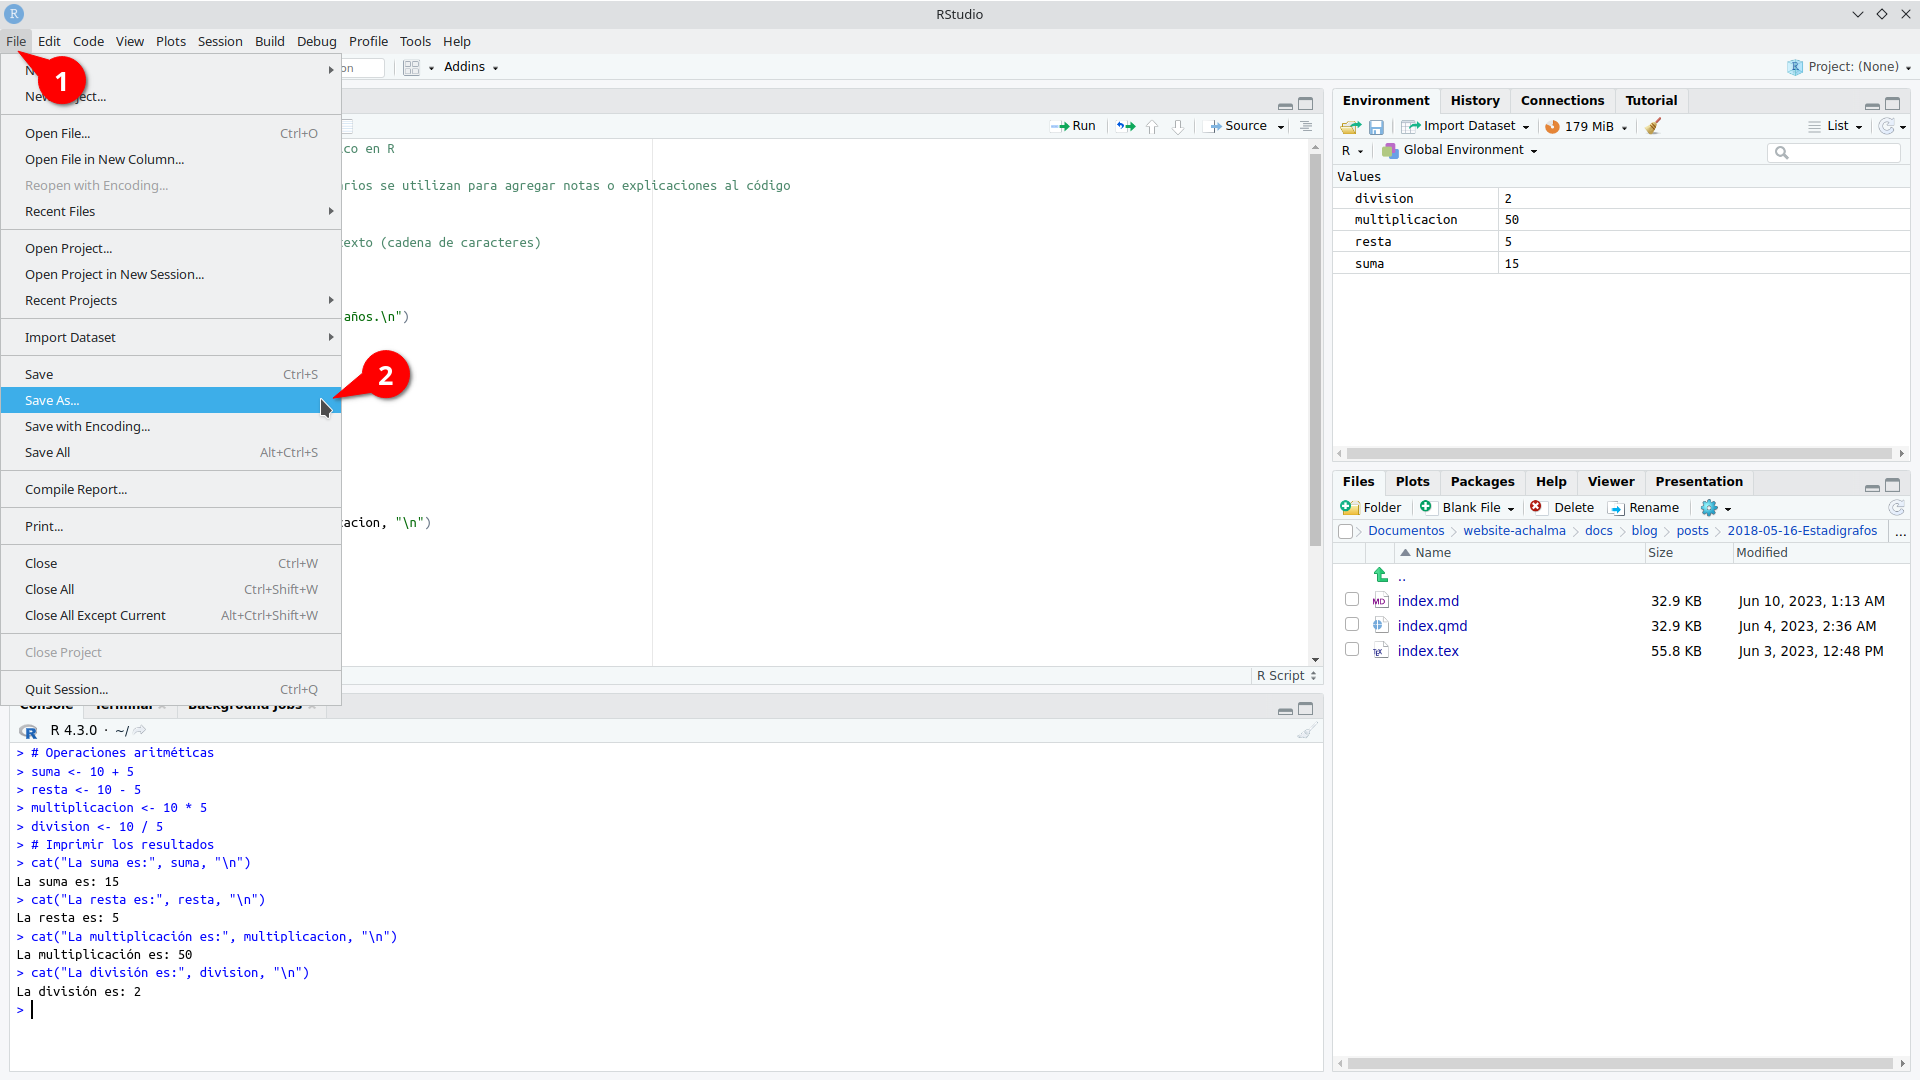
\includegraphics{2-Que-Ofrece-RStudio/images/Screenshot_20230611_010854.png}

Podemos elegir una ubicación y un nombre de archivo apropiados para
guardar nuestro script.

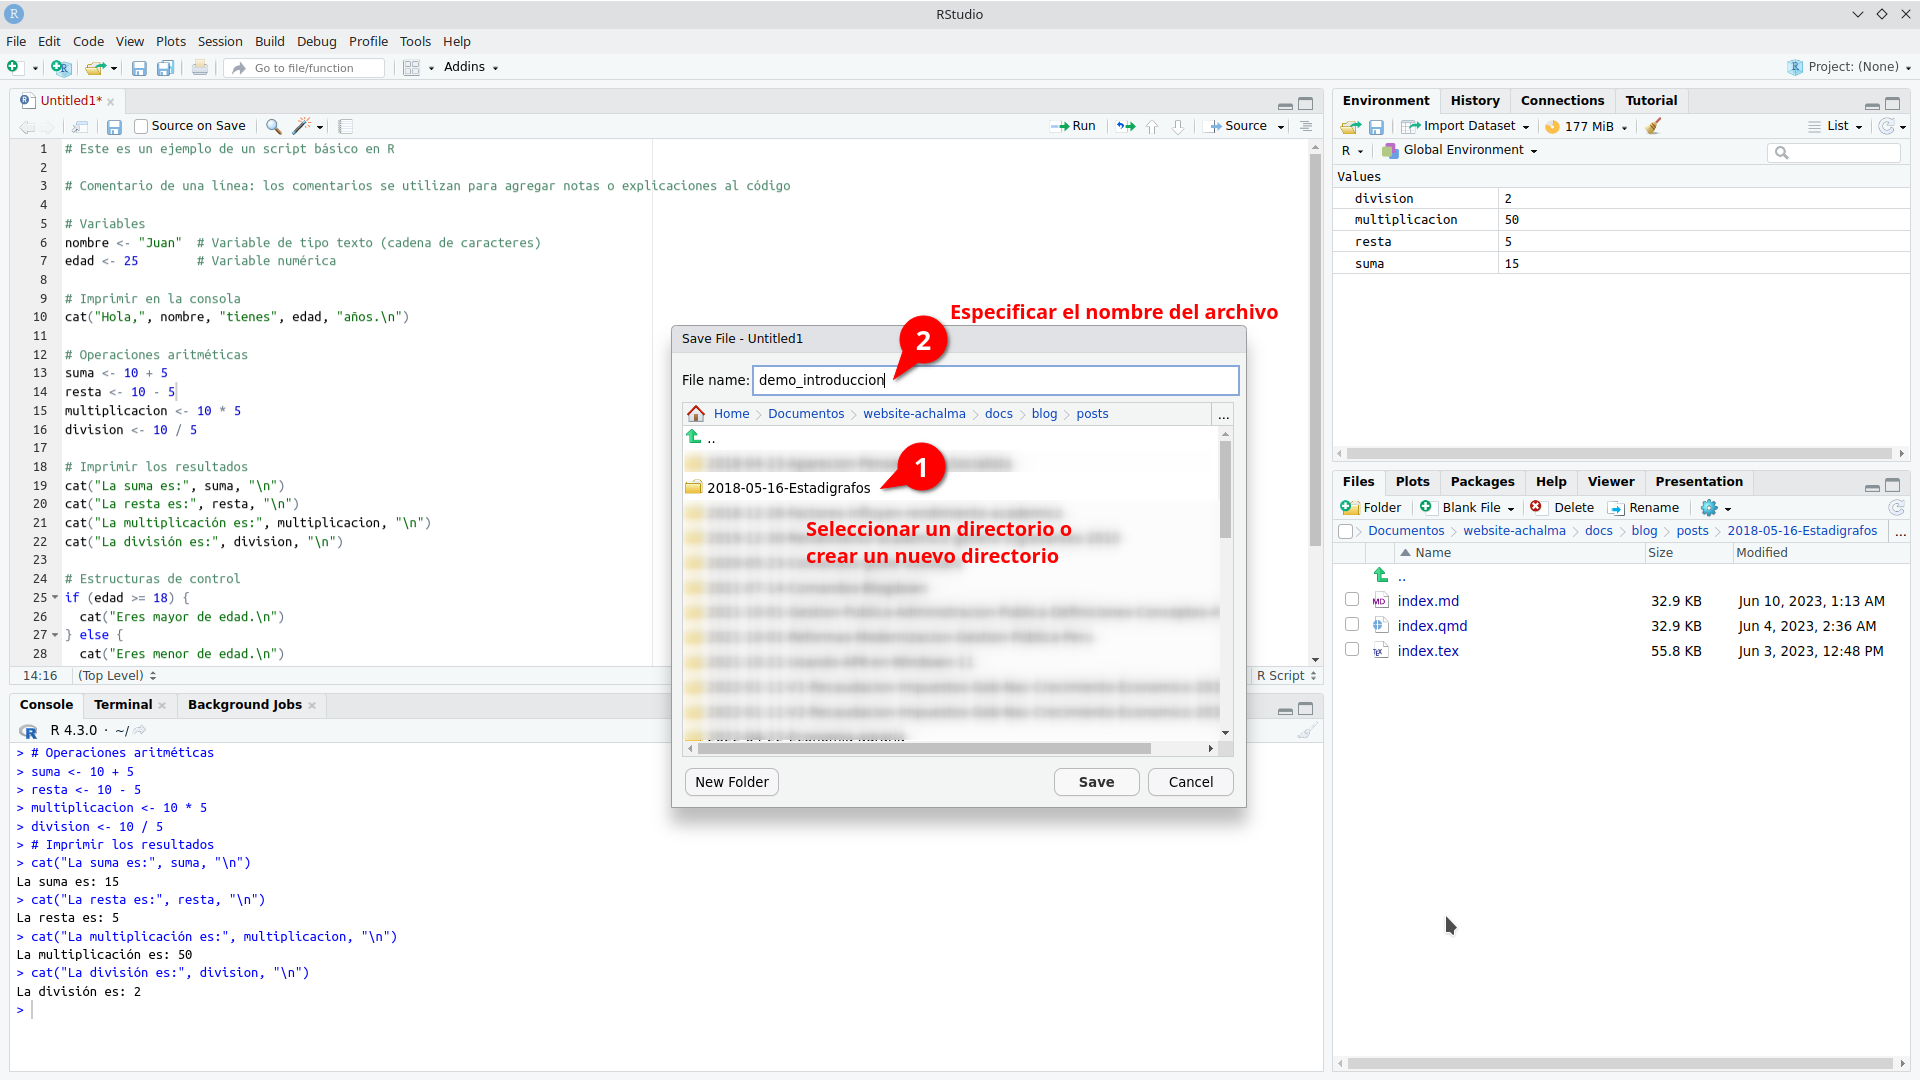
\includegraphics{2-Que-Ofrece-RStudio/images/Screenshot_20230611_012736.png}

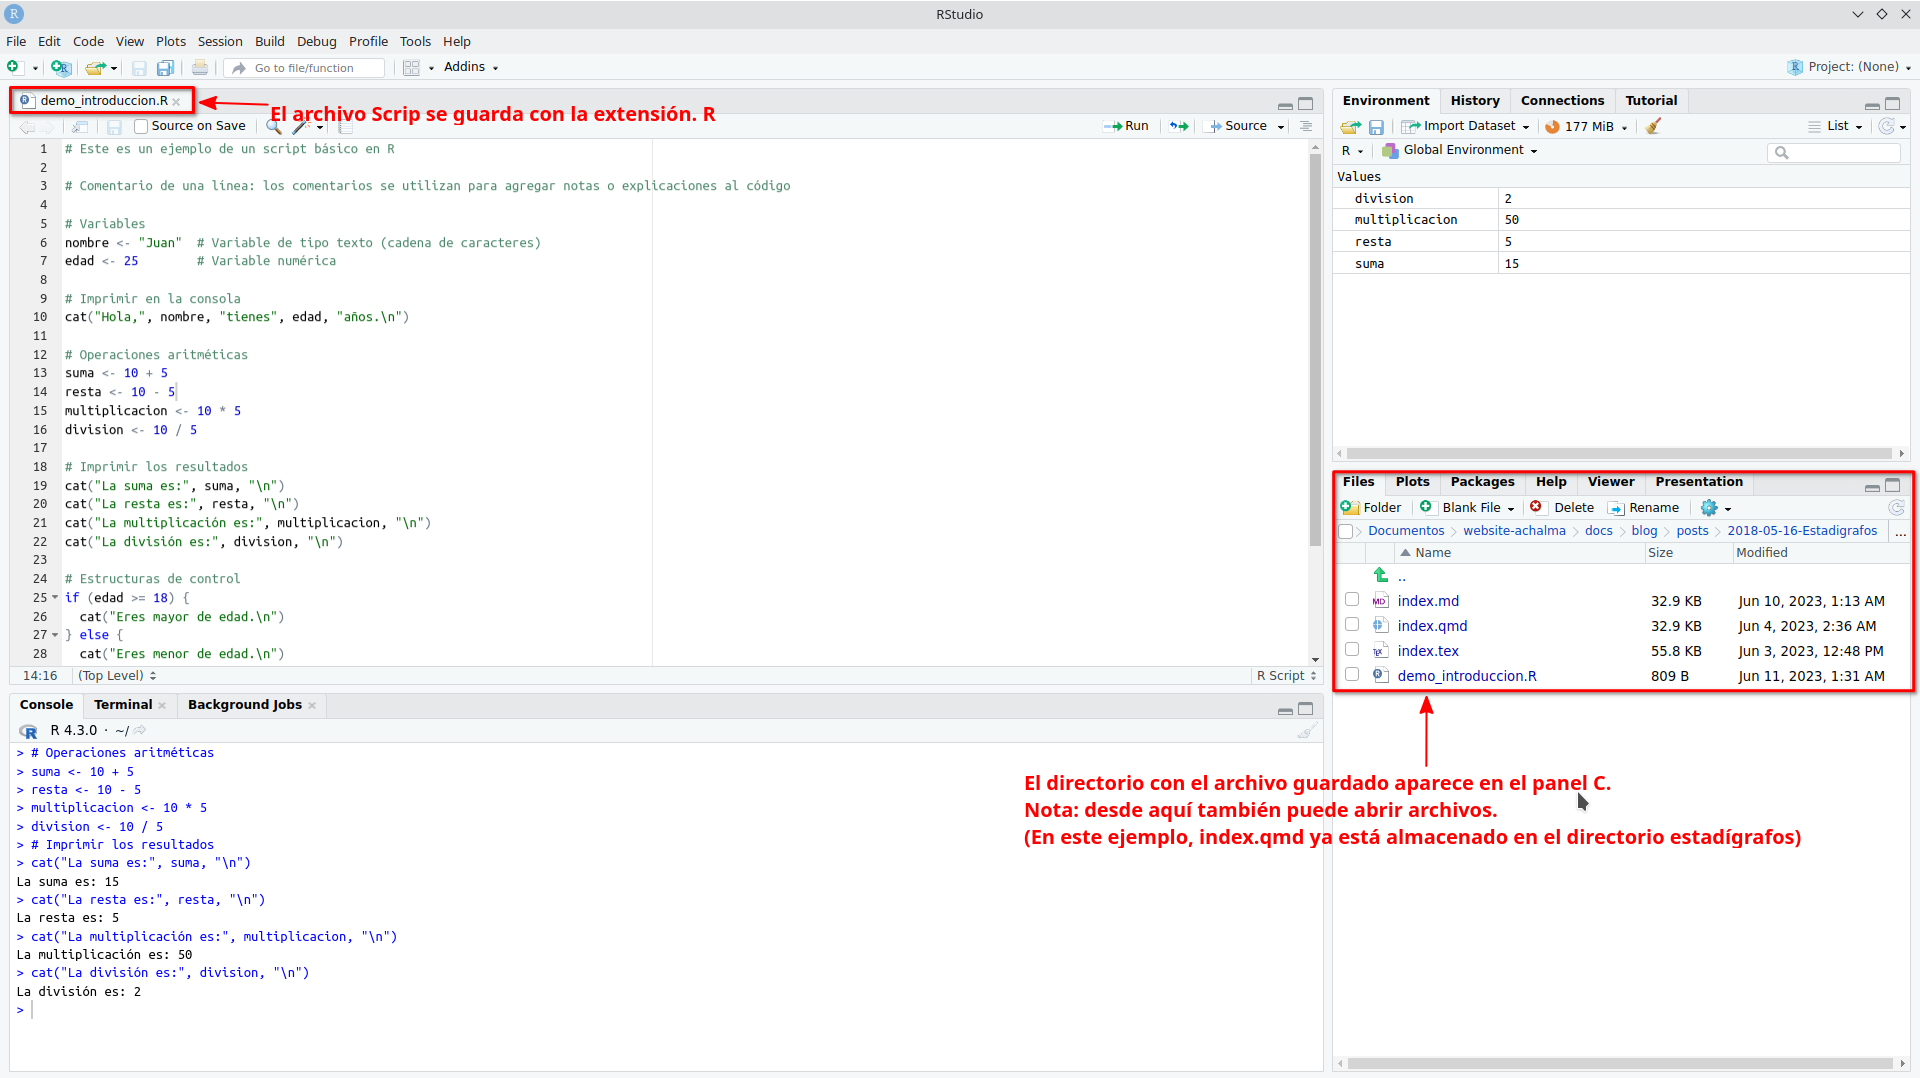
\includegraphics{2-Que-Ofrece-RStudio/images/Screenshot_20230611_013135.png}

\textbf{Paso 5: Continuar escribiendo y ejecutando el código}

Podemos continuar escribiendo y ejecutando más código en nuestro script
según nuestras necesidades. Podemos agregar nuevas líneas de código,
modificar las existentes o eliminar las que ya no necesitamos. Es
recomendable guardar el script regularmente a medida que realizamos
cambios.

\textbf{Paso 6: Exportar los resultados (opcional)}

Si deseamos guardar los resultados de nuestro análisis, podemos
exportarlos a archivos o formatos específicos. Por ejemplo, podemos
guardar tablas de datos en archivos CSV, gráficos en imágenes o informes
en formatos de texto. Esto nos permite compartir y utilizar los
resultados fuera de RStudio.

\begin{quote}
Recuerda que practicar y experimentar con diferentes comandos y
funciones en RStudio te ayudará a familiarizarte con el entorno y
mejorar tus habilidades de programación en R. ¡Diviértete explorando el
mundo del análisis de datos con RStudio!
\end{quote}

\hypertarget{shortcuts}{%
\section{Shortcuts}\label{shortcuts}}

Aquí tienes una tabla con algunos atajos de teclado útiles en RStudio
para usuarios de Ubuntu Linux:

\begin{longtable}[]{@{}
  >{\raggedright\arraybackslash}p{(\columnwidth - 2\tabcolsep) * \real{0.7222}}
  >{\raggedright\arraybackslash}p{(\columnwidth - 2\tabcolsep) * \real{0.2778}}@{}}
\toprule\noalign{}
\begin{minipage}[b]{\linewidth}\raggedright
Acción
\end{minipage} & \begin{minipage}[b]{\linewidth}\raggedright
Atajo de teclado
\end{minipage} \\
\midrule\noalign{}
\endhead
\bottomrule\noalign{}
\endlastfoot
Ejecutar el código / selección actual y saltar a la línea siguiente &
Ctrl + Enter \\
Ejecutar el código / selección actual y no saltar a la línea siguiente &
Alt + Enter \\
Ejecutar línea de código & Shift + Enter \\
Comentar/descomentar línea de código & Ctrl + Shift + C \\
Copiar línea de código & Ctrl + Shift + D \\
Pegar línea de código & Ctrl + Shift + V \\
Ir a la línea & Ctrl + G \\
Ir al inicio del documento & Ctrl + Home \\
Ir al final del documento & Ctrl + End \\
Completar código & Tab \\
Abrir ayuda & F1 \\
Guardar el archivo actual & Ctrl + S \\
Cerrar archivo & Ctrl + W \\
Deshacer & Ctrl + Z \\
Rehacer & Ctrl + Y \\
Abrir consola de R & Ctrl + Shift + Enter \\
Buscar en el archivo & Ctrl + F \\
Buscar y reemplazar en el archivo & Ctrl + Shift + F \\
Colapsar/expandir bloque de código & Ctrl + Shift + \\
Aumentar tamaño de fuente & Ctrl + + \\
Disminuir tamaño de fuente & Ctrl + - \\
Nuevo archivo Script R & Shift + Ctrl + N \\
Abrir archivo & Ctrl + O \\
Ejecutar todo el script & Ctrl + Alt + R \\
Ejecutar el código desde el principio hasta la línea actual & Ctrl + Alt
+ B \\
Ejecutar el código desde la línea actual hasta el final & Ctrl + Alt +
E \\
Mover el cursor al editor de código fuente & Ctrl + 1 \\
Mover el cursor a la consola & Ctrl + 2 \\
Eliminar selección actual & Ctrl + D \\
Limpiar consola & Ctrl + L \\
Navegar por el historial de la consola & arriba/abajo \\
Mover la línea de código arriba y abajo (evita el trabajo de copiar y
pegar) & Alt + arriba/abajo \\
Interrumpir el comando en ejecución & Esc \\
\end{longtable}

Estos atajos de teclado te ayudarán a agilizar tu flujo de trabajo en
RStudio en Ubuntu Linux. Recuerda que también puedes personalizar los
atajos de teclado según tus preferencias en la sección de configuración
de RStudio.

\hypertarget{espacio-de-trabajo-.rdata}{%
\section{Espacio de trabajo (.Rdata)}\label{espacio-de-trabajo-.rdata}}

El espacio de trabajo en R consiste en todos los objetos que se crean o
cargan durante una sesión de R.

\hypertarget{creaciuxf3n-de-objetos-de-datos}{%
\subsection{Creación de objetos de
datos}\label{creaciuxf3n-de-objetos-de-datos}}

\begin{enumerate}
\def\labelenumi{\arabic{enumi}.}
\tightlist
\item
  Utiliza el operador de asignación (\texttt{\textless{}-}) para crear
  un objeto de datos. Por ejemplo:
  \texttt{mi\_objeto\ \textless{}-\ c(1,\ 2,\ 3,\ 4,\ 5)}.
\end{enumerate}

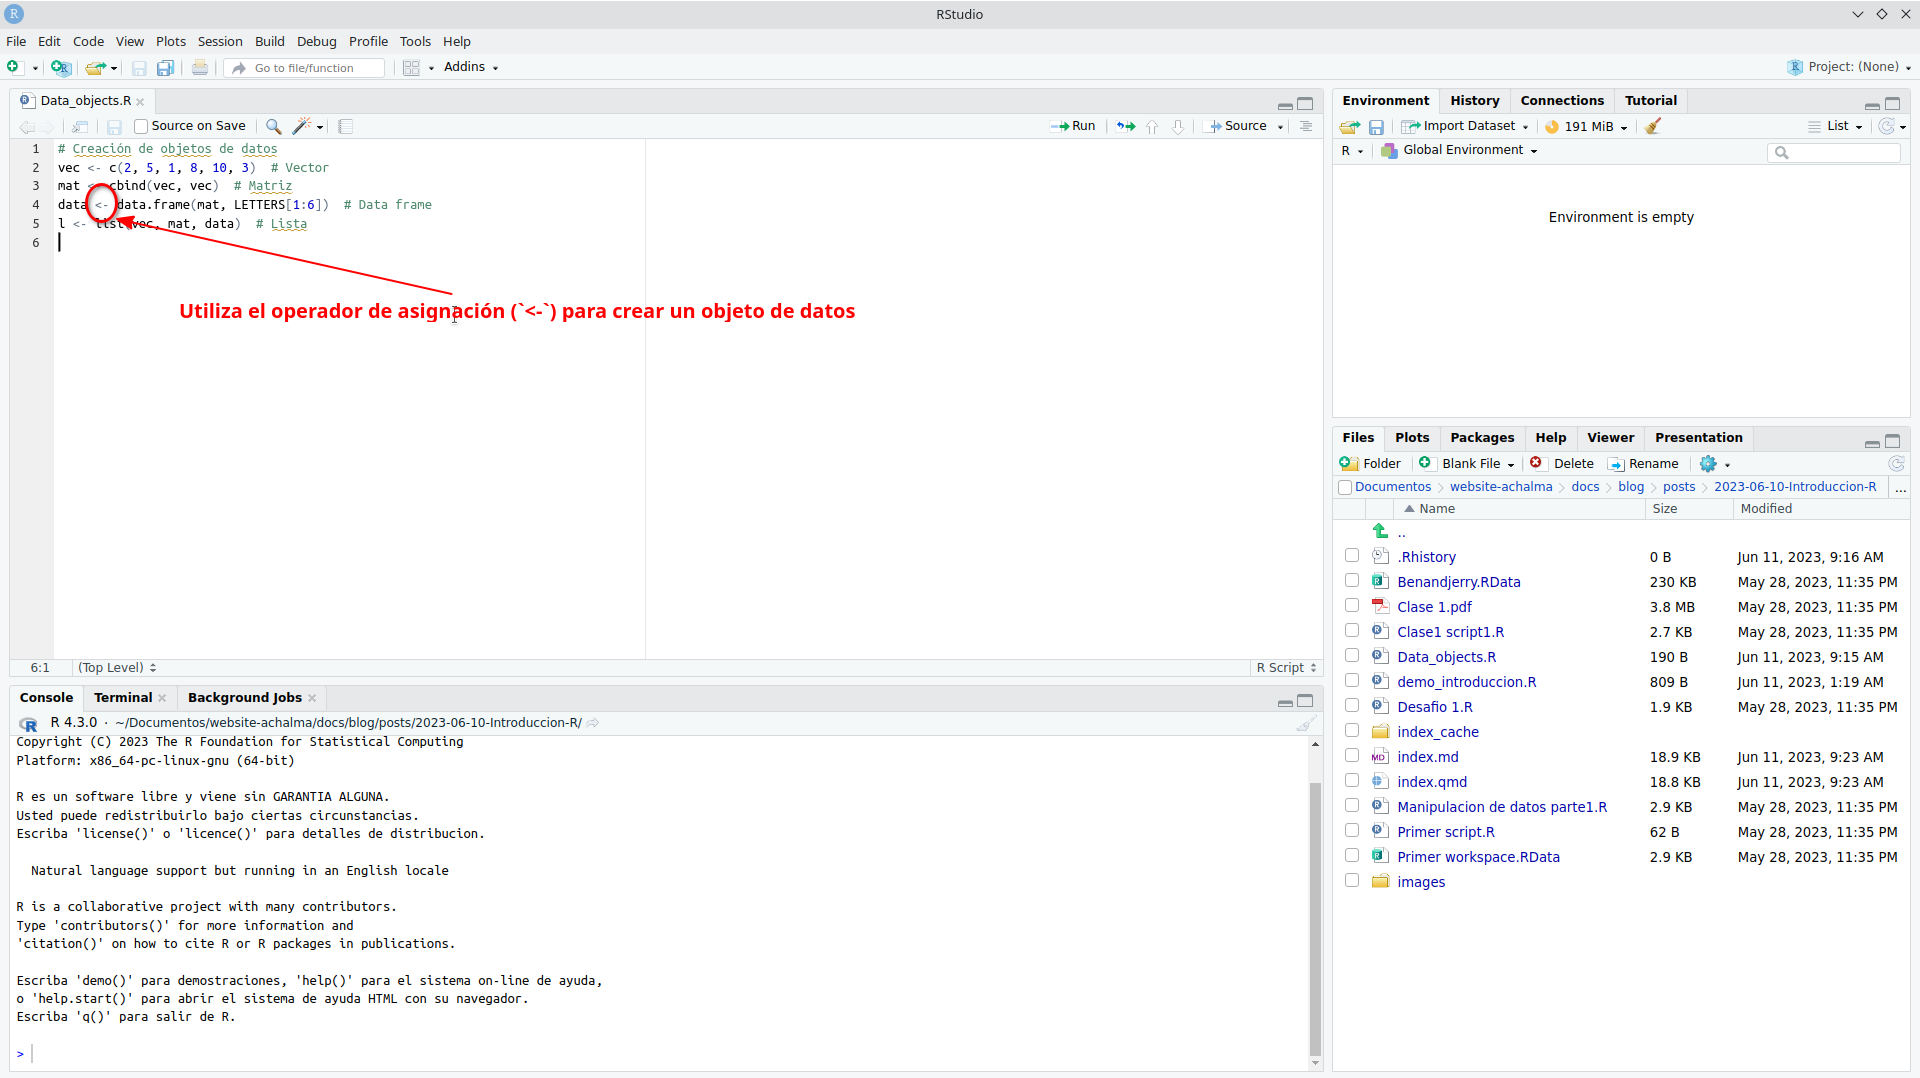
\includegraphics{2-Que-Ofrece-RStudio/images/Screenshot_20230611_092644.png}

\begin{enumerate}
\def\labelenumi{\arabic{enumi}.}
\setcounter{enumi}{1}
\tightlist
\item
  Selecciona todo el código que contiene los objetos de datos y
  ejecútalo en la consola de RStudio.
\end{enumerate}

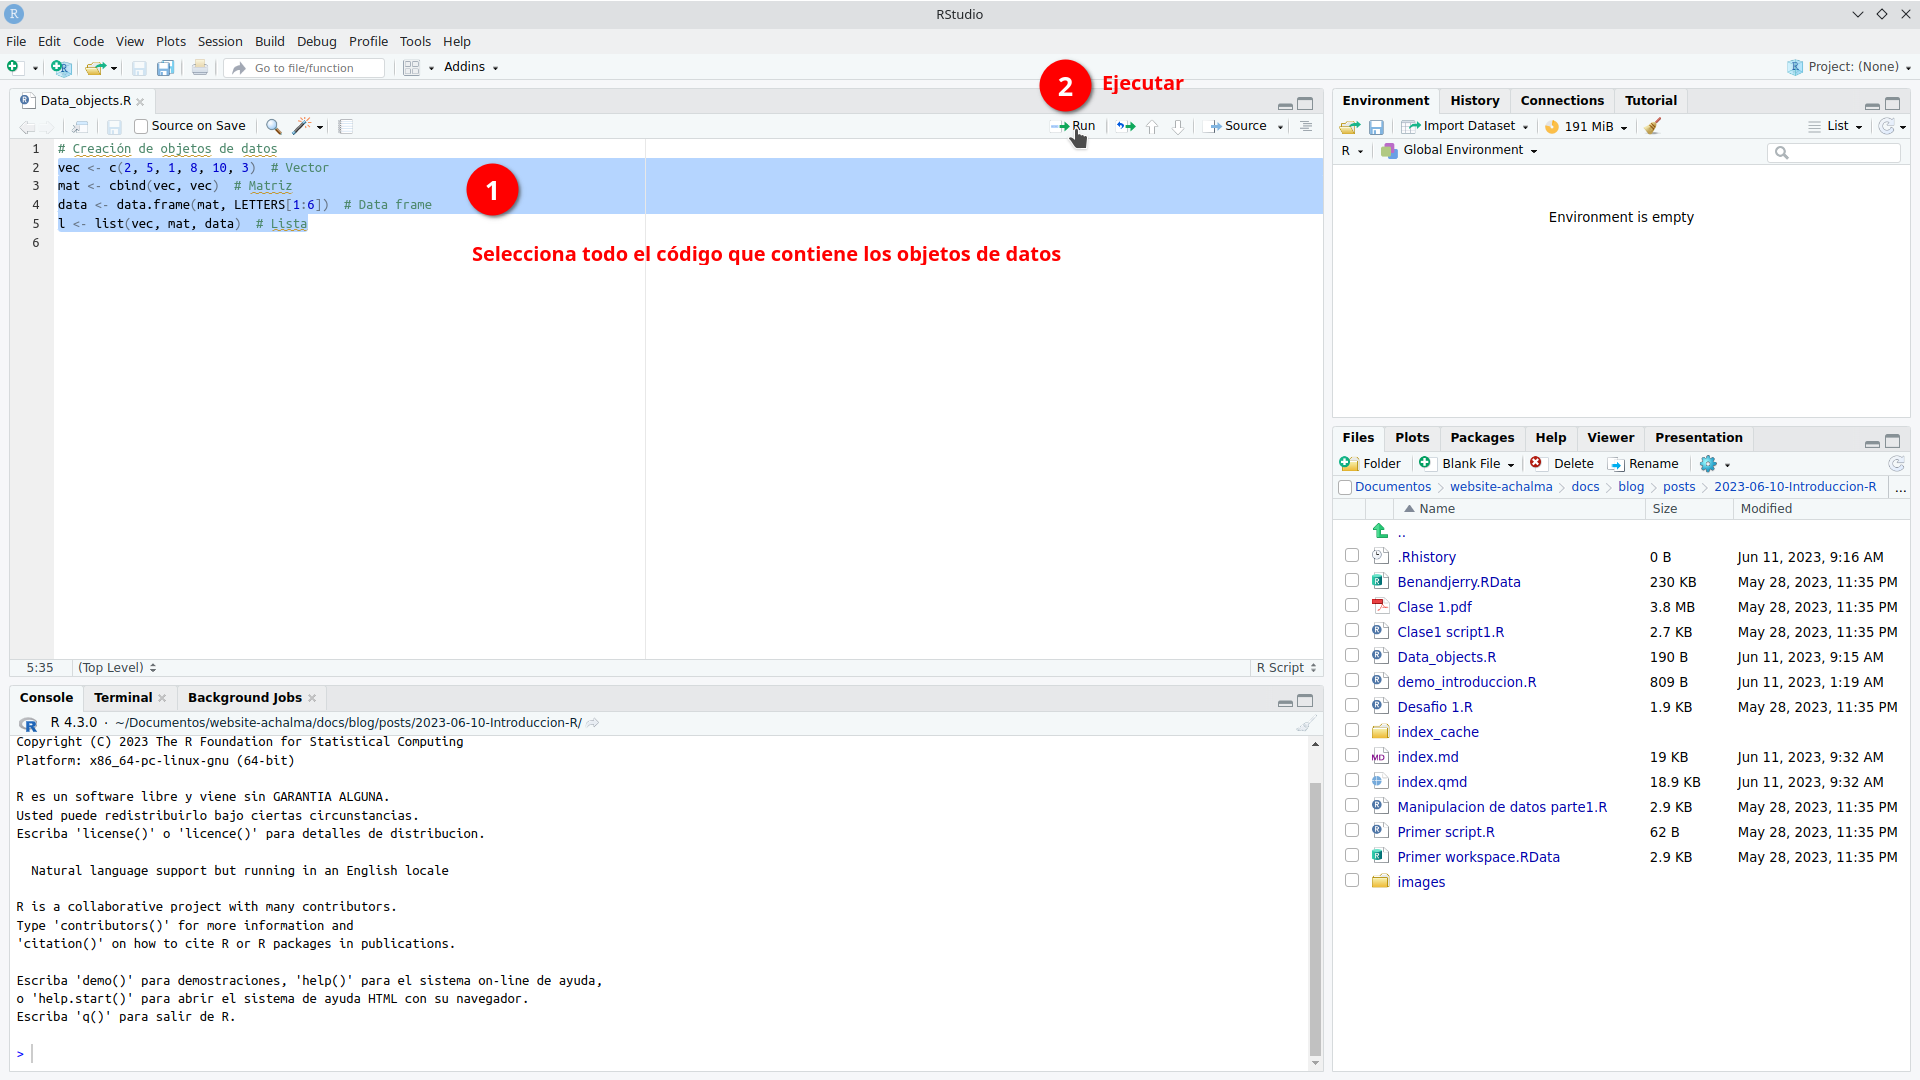
\includegraphics{2-Que-Ofrece-RStudio/images/Screenshot_20230611_093536.png}

\begin{enumerate}
\def\labelenumi{\arabic{enumi}.}
\setcounter{enumi}{2}
\tightlist
\item
  El código se evaluará y los objetos de datos se crearán en el espacio
  de trabajo. Sin embargo, no verás ningún resultado en la consola.
\end{enumerate}

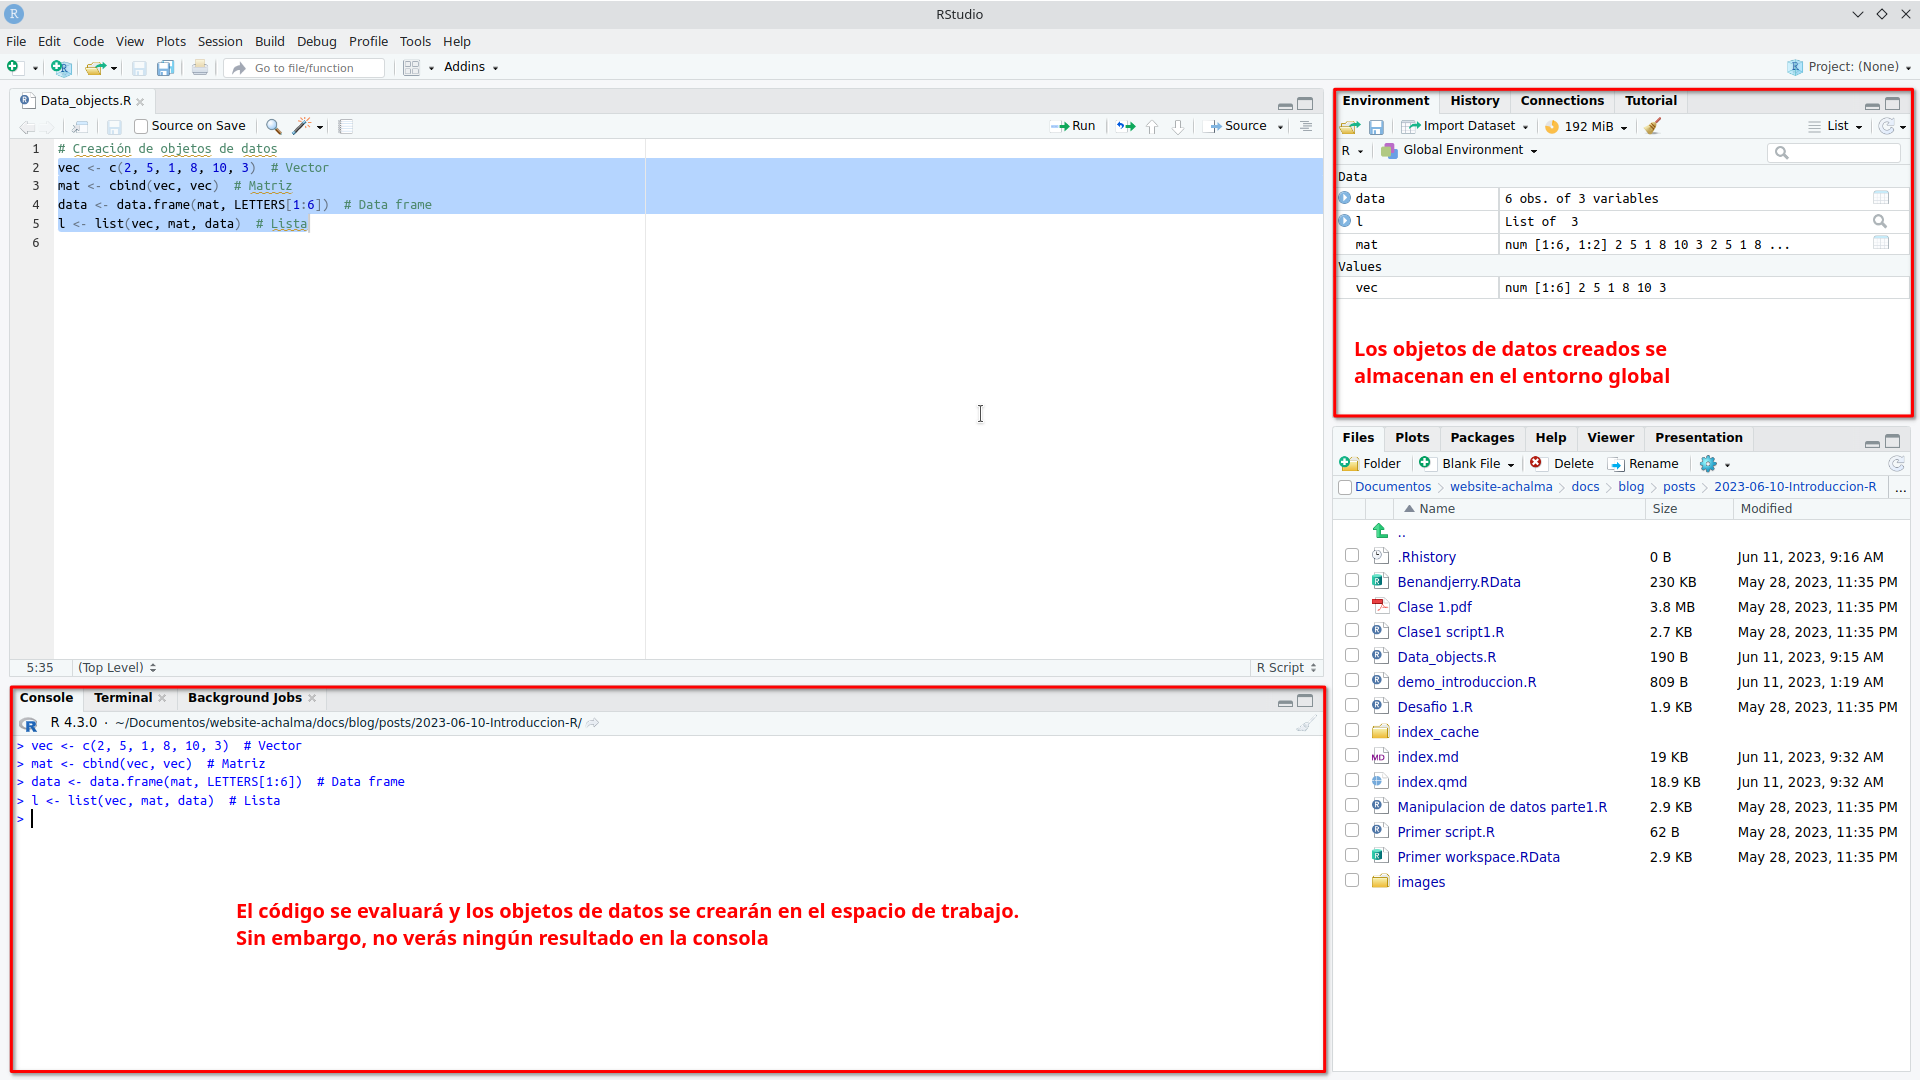
\includegraphics{2-Que-Ofrece-RStudio/images/Screenshot_20230611_094001.png}

Los objetos de datos creados se almacenan en el entorno global, que es
parte del espacio de trabajo de R.

\hypertarget{inspecciuxf3n-de-objetos-de-datos}{%
\subsection{Inspección de objetos de
datos}\label{inspecciuxf3n-de-objetos-de-datos}}

Puedes inspeccionar los objetos de datos haciendo clic sobre ellos en el
panel de entorno o en el panel de objetos. Esto abrirá una vista previa
del objeto en un nuevo archivo. Ten en cuenta que esta vista previa no
afecta los objetos en el espacio de trabajo y se puede cerrar sin perder
ninguna información.

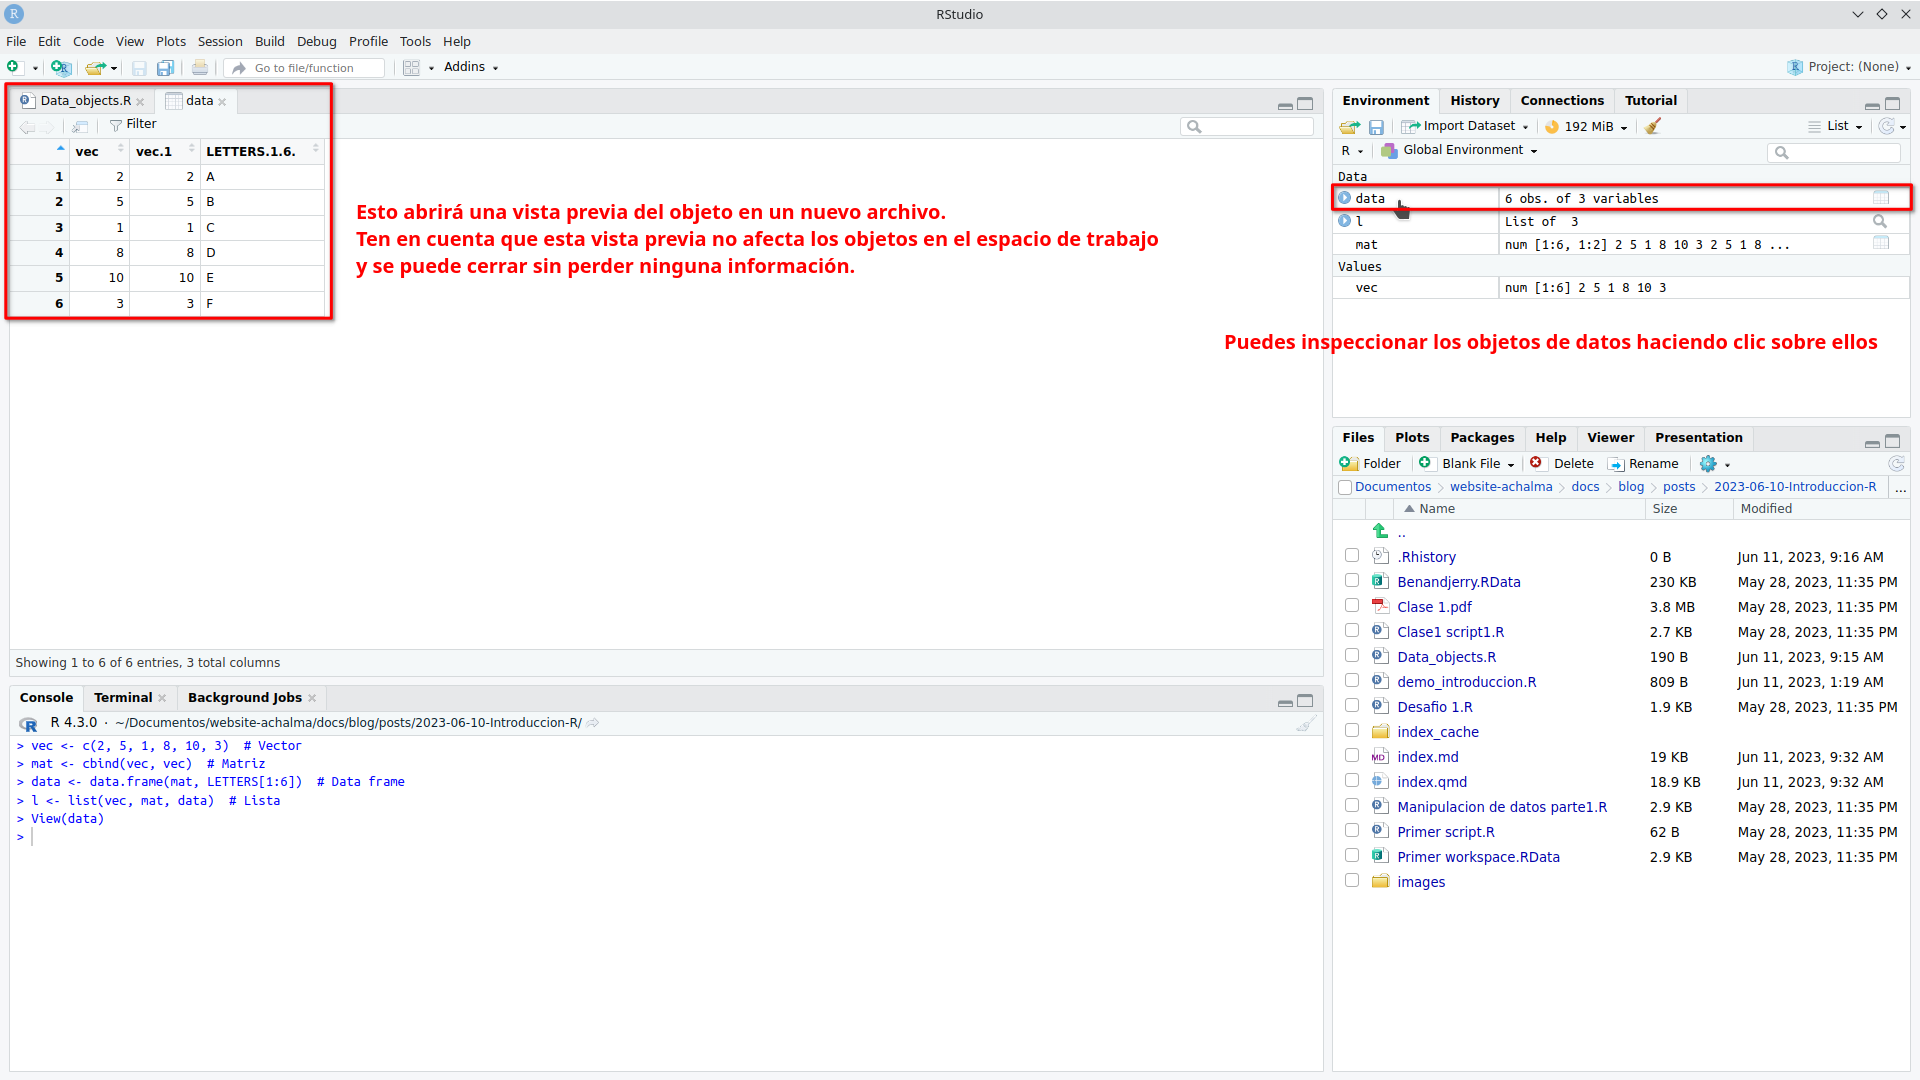
\includegraphics{2-Que-Ofrece-RStudio/images/Screenshot_20230611_094530.png}

\hypertarget{guardado-del-espacio-de-trabajo}{%
\subsection{Guardado del espacio de
trabajo}\label{guardado-del-espacio-de-trabajo}}

En RStudio, puedes guardar todos los objetos en tu espacio de trabajo en
un archivo llamado \texttt{.Rdata}. Esta función te permite almacenar y
cargar el espacio de trabajo completo en futuras sesiones de RStudio.

Para guardar el espacio de trabajo, simplemente ve al menú ``Session'' y
selecciona ``Save Workspace As\ldots{}''. A continuación, elige la
ubicación y el nombre de archivo deseados para guardar el archivo
\texttt{.Rdata}.

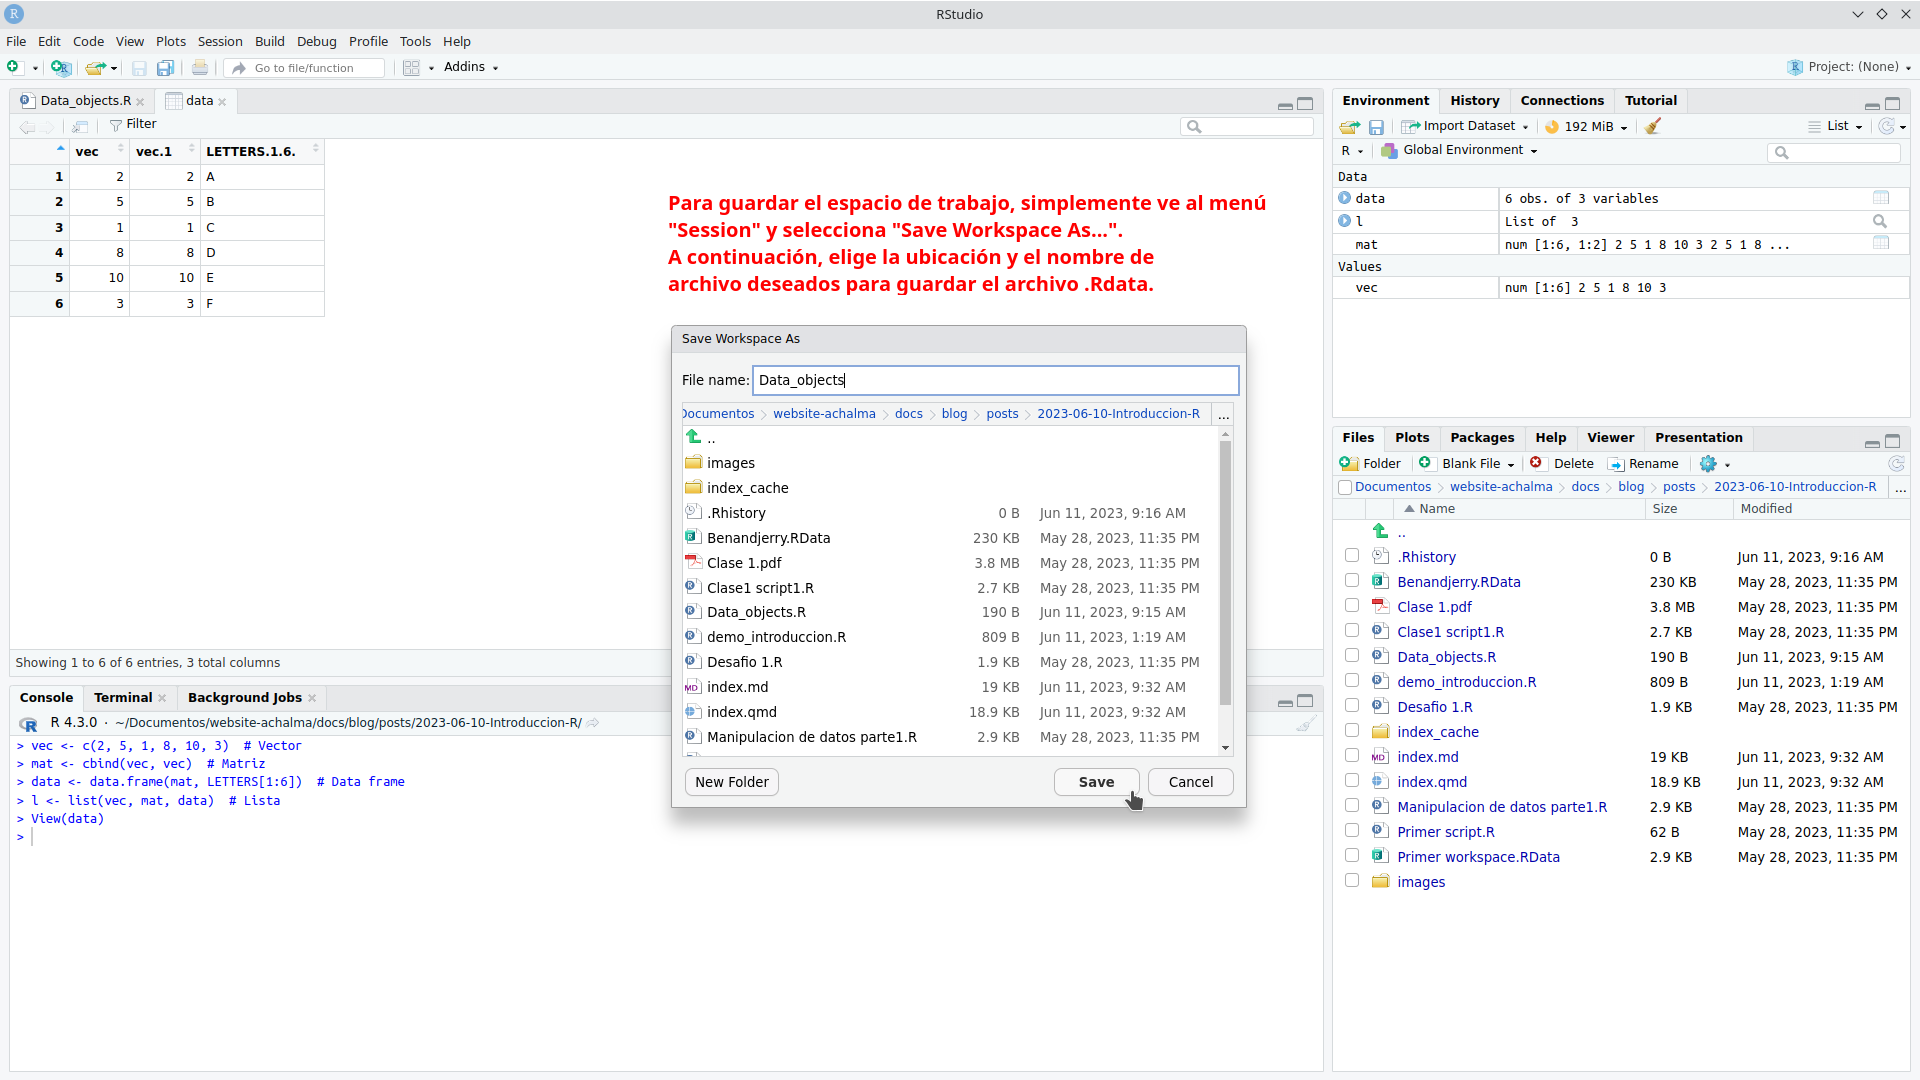
\includegraphics{2-Que-Ofrece-RStudio/images/Screenshot_20230611_095350.png}

Esta función es especialmente útil cuando trabajas en proyectos largos o
cuando deseas retomar tu trabajo en otro momento sin tener que volver a
crear o cargar manualmente todos los objetos y configuraciones.

\begin{quote}
Recuerda que al guardar y cargar el espacio de trabajo, asegúrate de
mantener un respaldo de tus archivos en caso de cualquier eventualidad.
¡Disfruta de la conveniencia de mantener tus objetos y configuraciones
en tu espacio de trabajo guardado!
\end{quote}

\hypertarget{carga-del-espacio-de-trabajo}{%
\subsection{Carga del espacio de
trabajo}\label{carga-del-espacio-de-trabajo}}

Para cargar el espacio de trabajo previamente guardado, sigue estos
pasos:

\begin{enumerate}
\def\labelenumi{\arabic{enumi}.}
\tightlist
\item
  Abre RStudio y ve al menú ``Session'' en la barra de herramientas
  superior.
\item
  Selecciona la opción ``Cargar'' del menú desplegable.
\item
  Aparecerá una ventana emergente que te permite buscar el archivo
  \texttt{.Rdata} que contiene tu espacio de trabajo guardado. Navega
  hasta la ubicación donde guardaste el archivo.
\item
  Selecciona el archivo \texttt{.Rdata} y haz clic en el botón
  ``Abrir''.
\item
  RStudio cargará automáticamente el archivo y restaurará todos los
  objetos y sus valores en tu entorno de trabajo actual.
\end{enumerate}

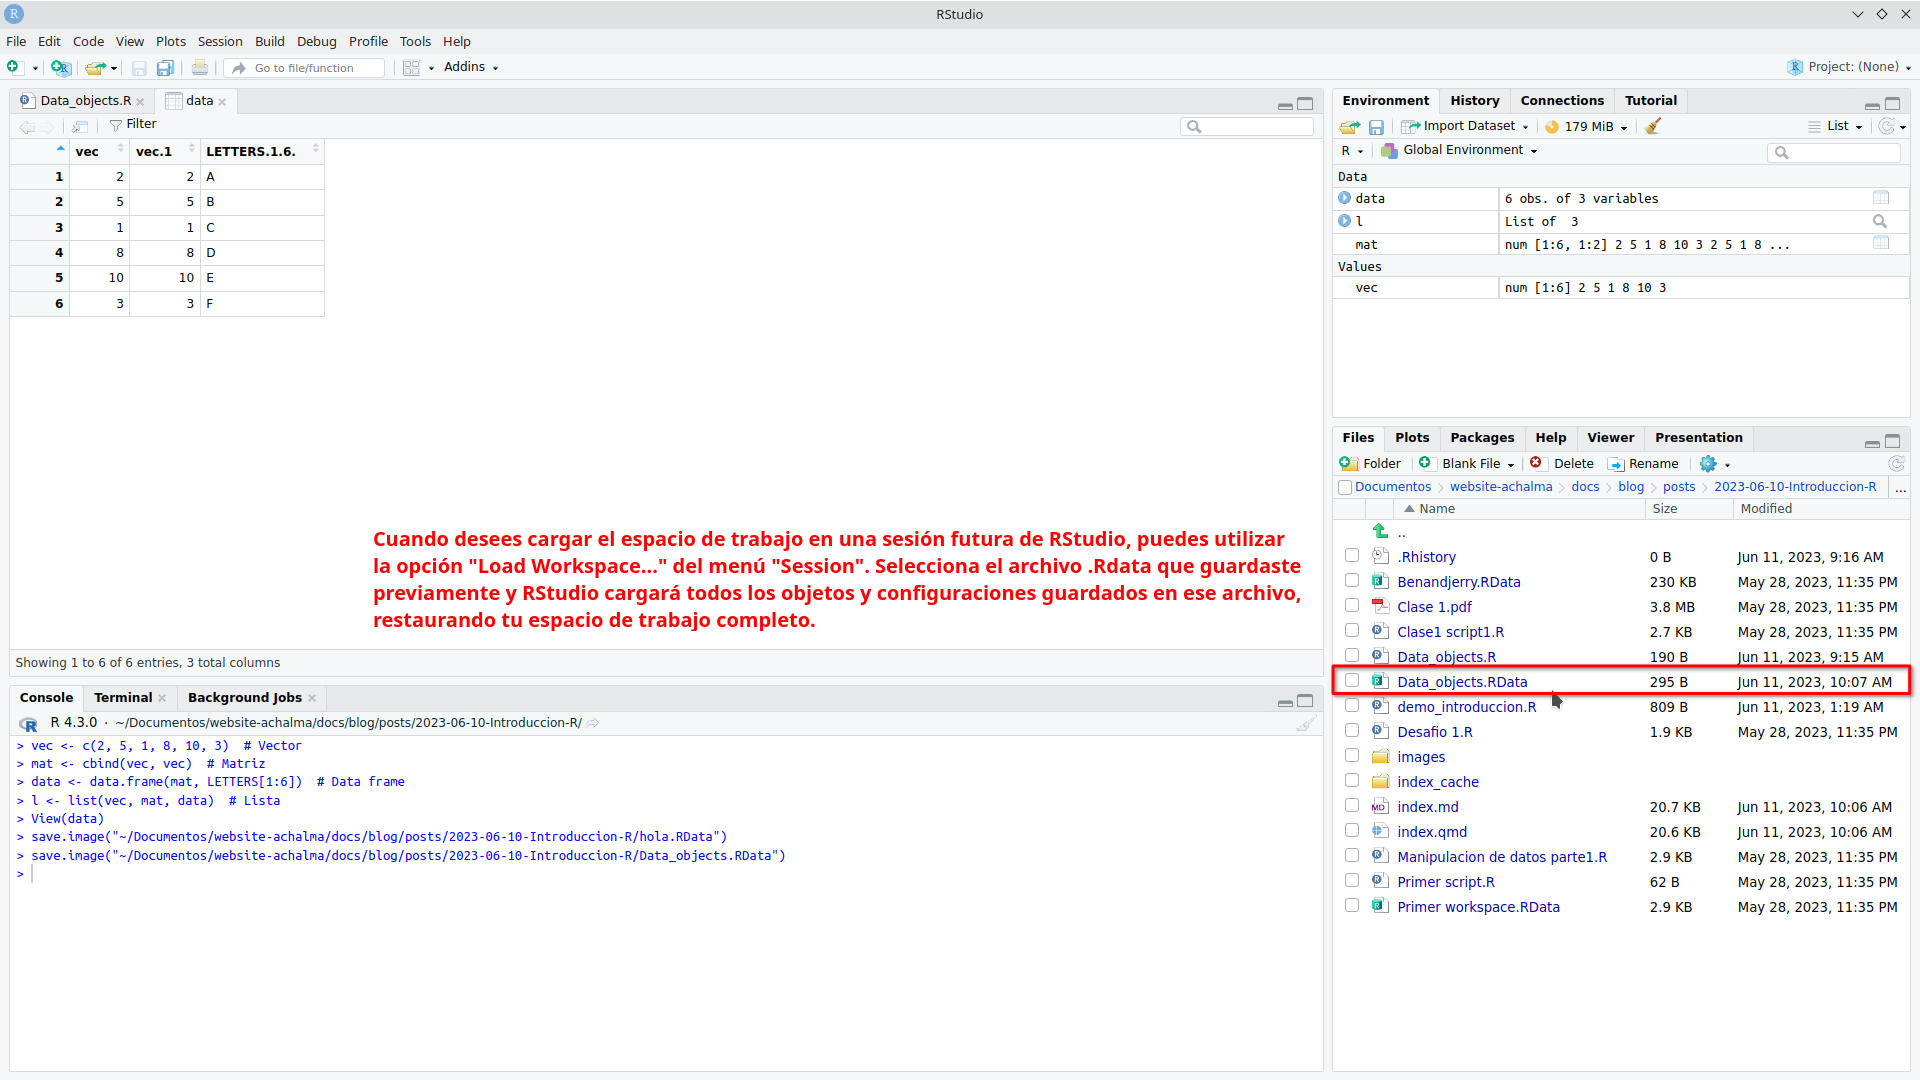
\includegraphics{2-Que-Ofrece-RStudio/images/Screenshot_20230611_100949.png}

Una vez completados estos pasos, podrás acceder a todos los objetos y
continuar trabajando con ellos como lo hiciste en la sesión en la que
guardaste el espacio de trabajo.

\begin{quote}
¡Con esta opción de carga, podrás retomar fácilmente tus proyectos
anteriores y continuar donde lo dejaste sin tener que volver a crear los
objetos desde cero!
\end{quote}

\hypertarget{historial-.rhistory}{%
\section{Historial (.Rhistory)}\label{historial-.rhistory}}

El archivo de historial es un archivo de texto que registra todos los
comandos ejecutados durante una sesión de RStudio.

\hypertarget{inspecciuxf3n-del-historial-de-comandos}{%
\subsection{Inspección del historial de
comandos}\label{inspecciuxf3n-del-historial-de-comandos}}

Puedes ver el historial de comandos ejecutados durante tu sesión de
trabajo haciendo clic en la pestaña ``History'' en la parte superior
derecha de la ventana de RStudio. Aquí encontrarás una lista de todos
los comandos ejecutados, lo que te permite revisarlos y volver a
utilizarlos según sea necesario.

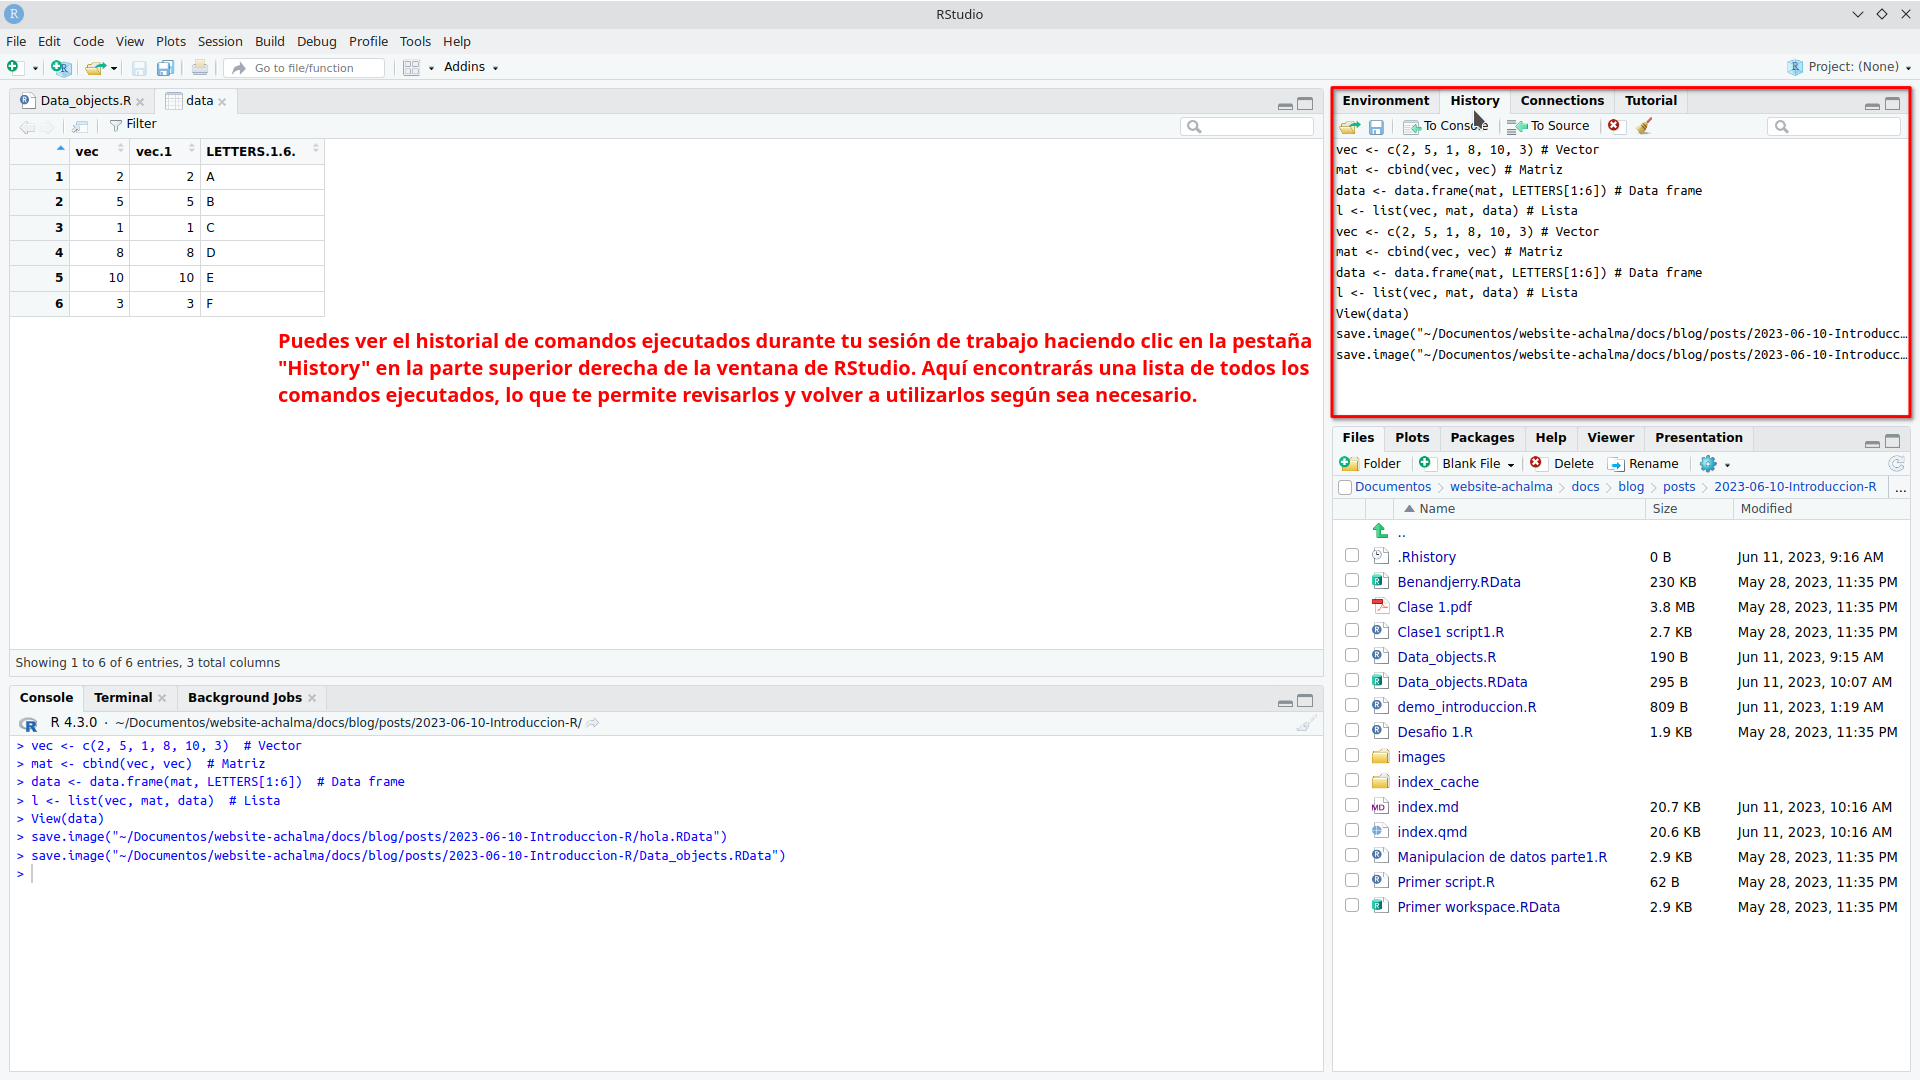
\includegraphics{2-Que-Ofrece-RStudio/images/Screenshot_20230611_101644.png}

\hypertarget{guardado-del-historial-de-comandos}{%
\subsection{Guardado del historial de
comandos}\label{guardado-del-historial-de-comandos}}

Si deseas guardar tu historial de comandos, puedes hacerlo en cualquier
momento durante tu sesión de trabajo. Esto te permitirá acceder a tus
comandos previos en futuras sesiones.

Si deseas guardar tu historial de comandos en RStudio, sigue estos
pasos:

\begin{enumerate}
\def\labelenumi{\arabic{enumi}.}
\tightlist
\item
  En el panel de superior derecha selecciona la opción ``Save History''
  (Guardar Historial).
\item
  Aparecerá una ventana emergente que te permitirá seleccionar la
  ubicación y el nombre de archivo para guardar tu historial de
  comandos. El archivo tendrá una extensión \texttt{.Rhistory} por
  defecto.
\item
  Elige la ubicación donde deseas guardar el archivo y asigna un nombre
  descriptivo para identificarlo fácilmente.
\item
  Haz clic en el botón ``Guardar'' para guardar el historial de comandos
  en el archivo seleccionado.
\end{enumerate}

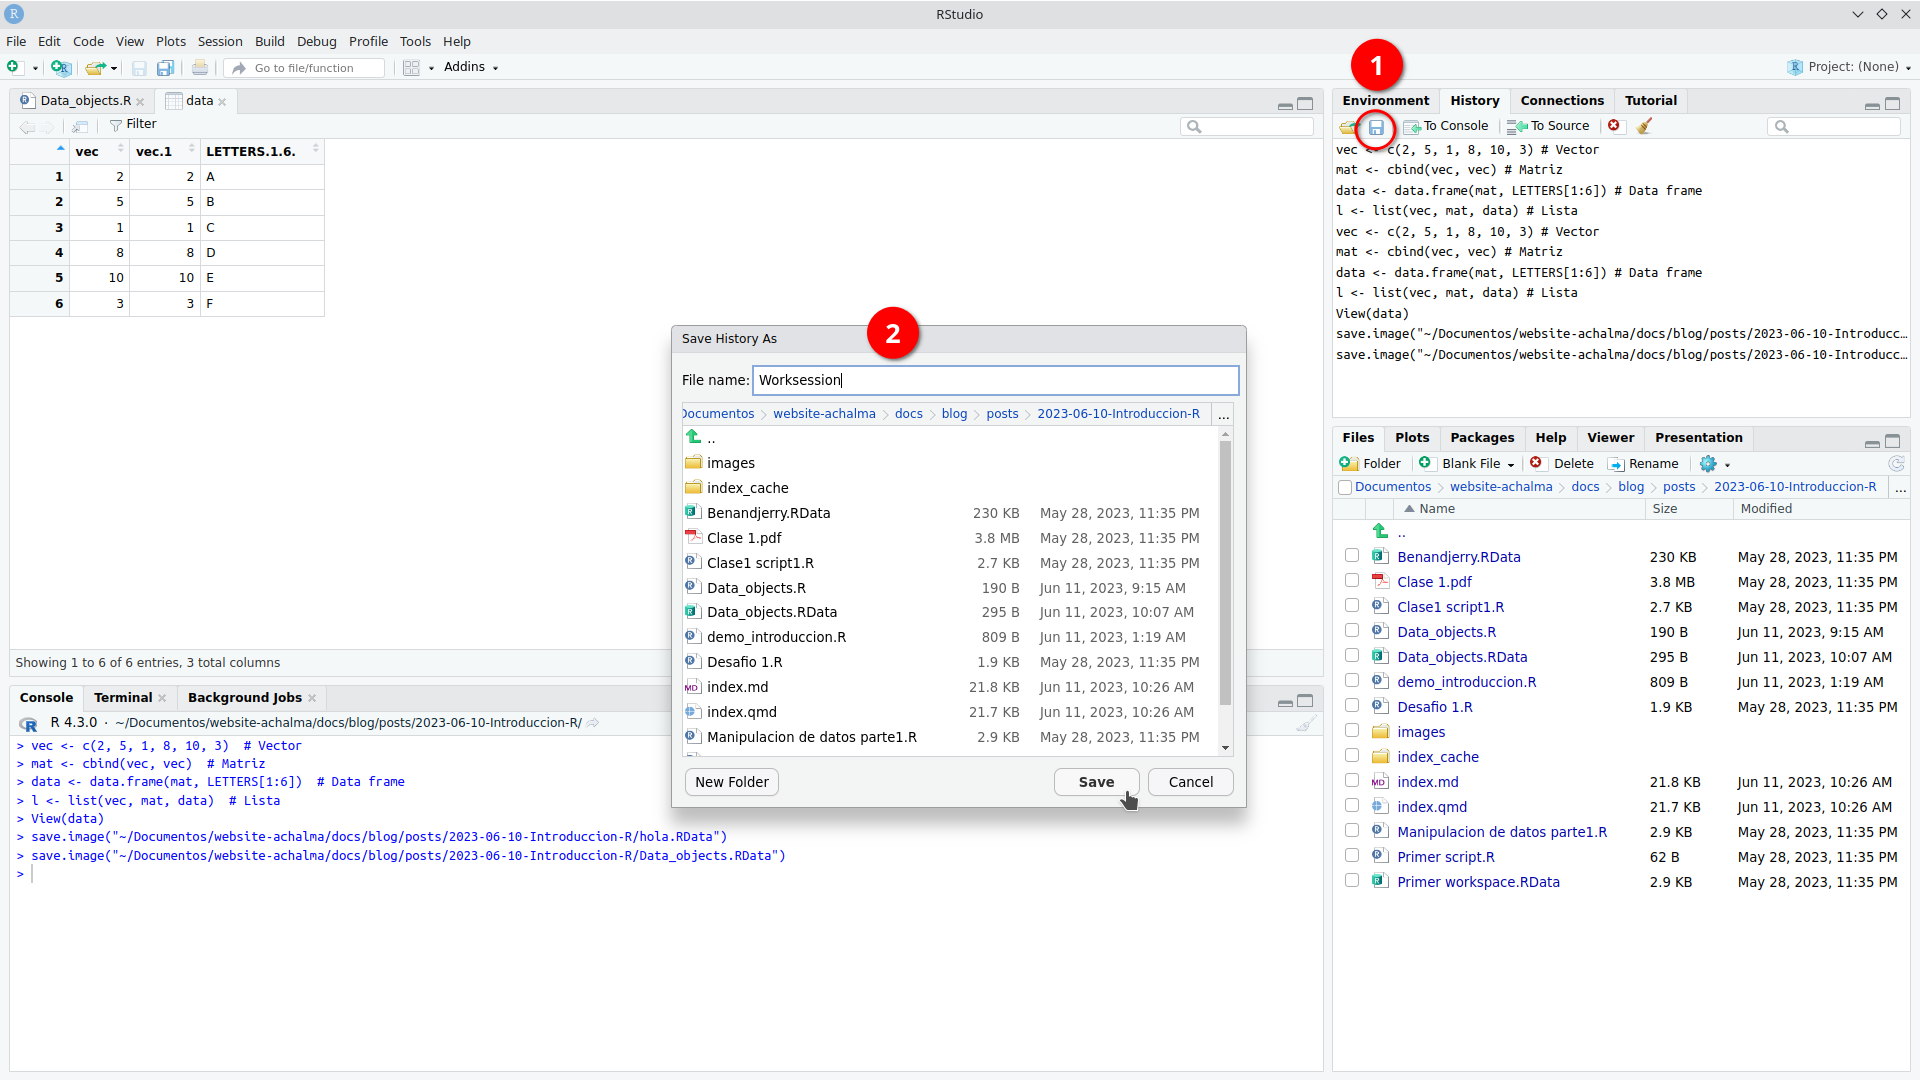
\includegraphics{2-Que-Ofrece-RStudio/images/Screenshot_20230611_102856.png}

\hypertarget{reutilizaciuxf3n-del-historial-de-comandos}{%
\subsection{Reutilización del historial de
comandos}\label{reutilizaciuxf3n-del-historial-de-comandos}}

El historial se guarda en un archivo llamado \texttt{.Rhistory}. Puedes
reutilizar todo el historial de comandos haciendo clic en el archivo
\texttt{.Rhistory} o con el nombre asignado. Luego, puedes copiarlos y
pegarlos en tu archivo de script actual.

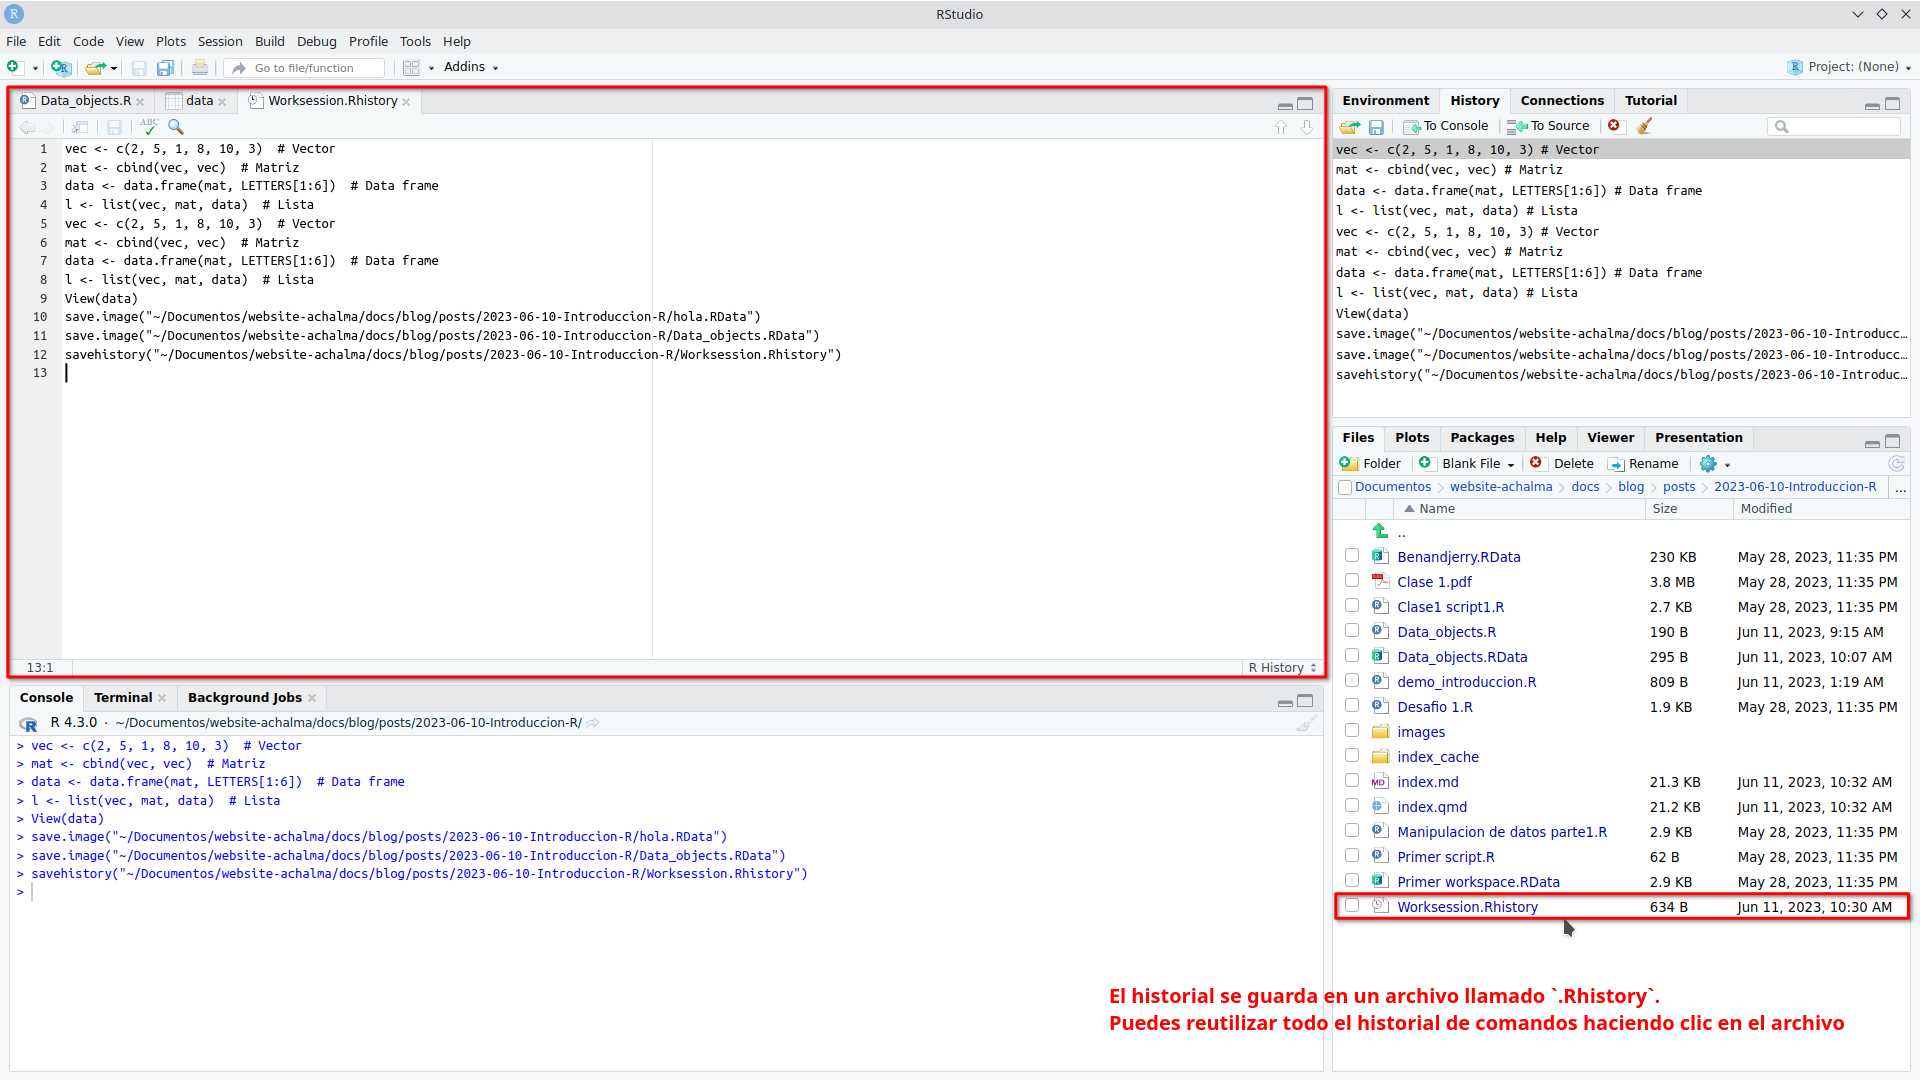
\includegraphics{2-Que-Ofrece-RStudio/images/Screenshot_20230611_103319.png}

Inserta un código de línea seleccionado de \texttt{.Rhistory} en un
archivo de script nuevo.

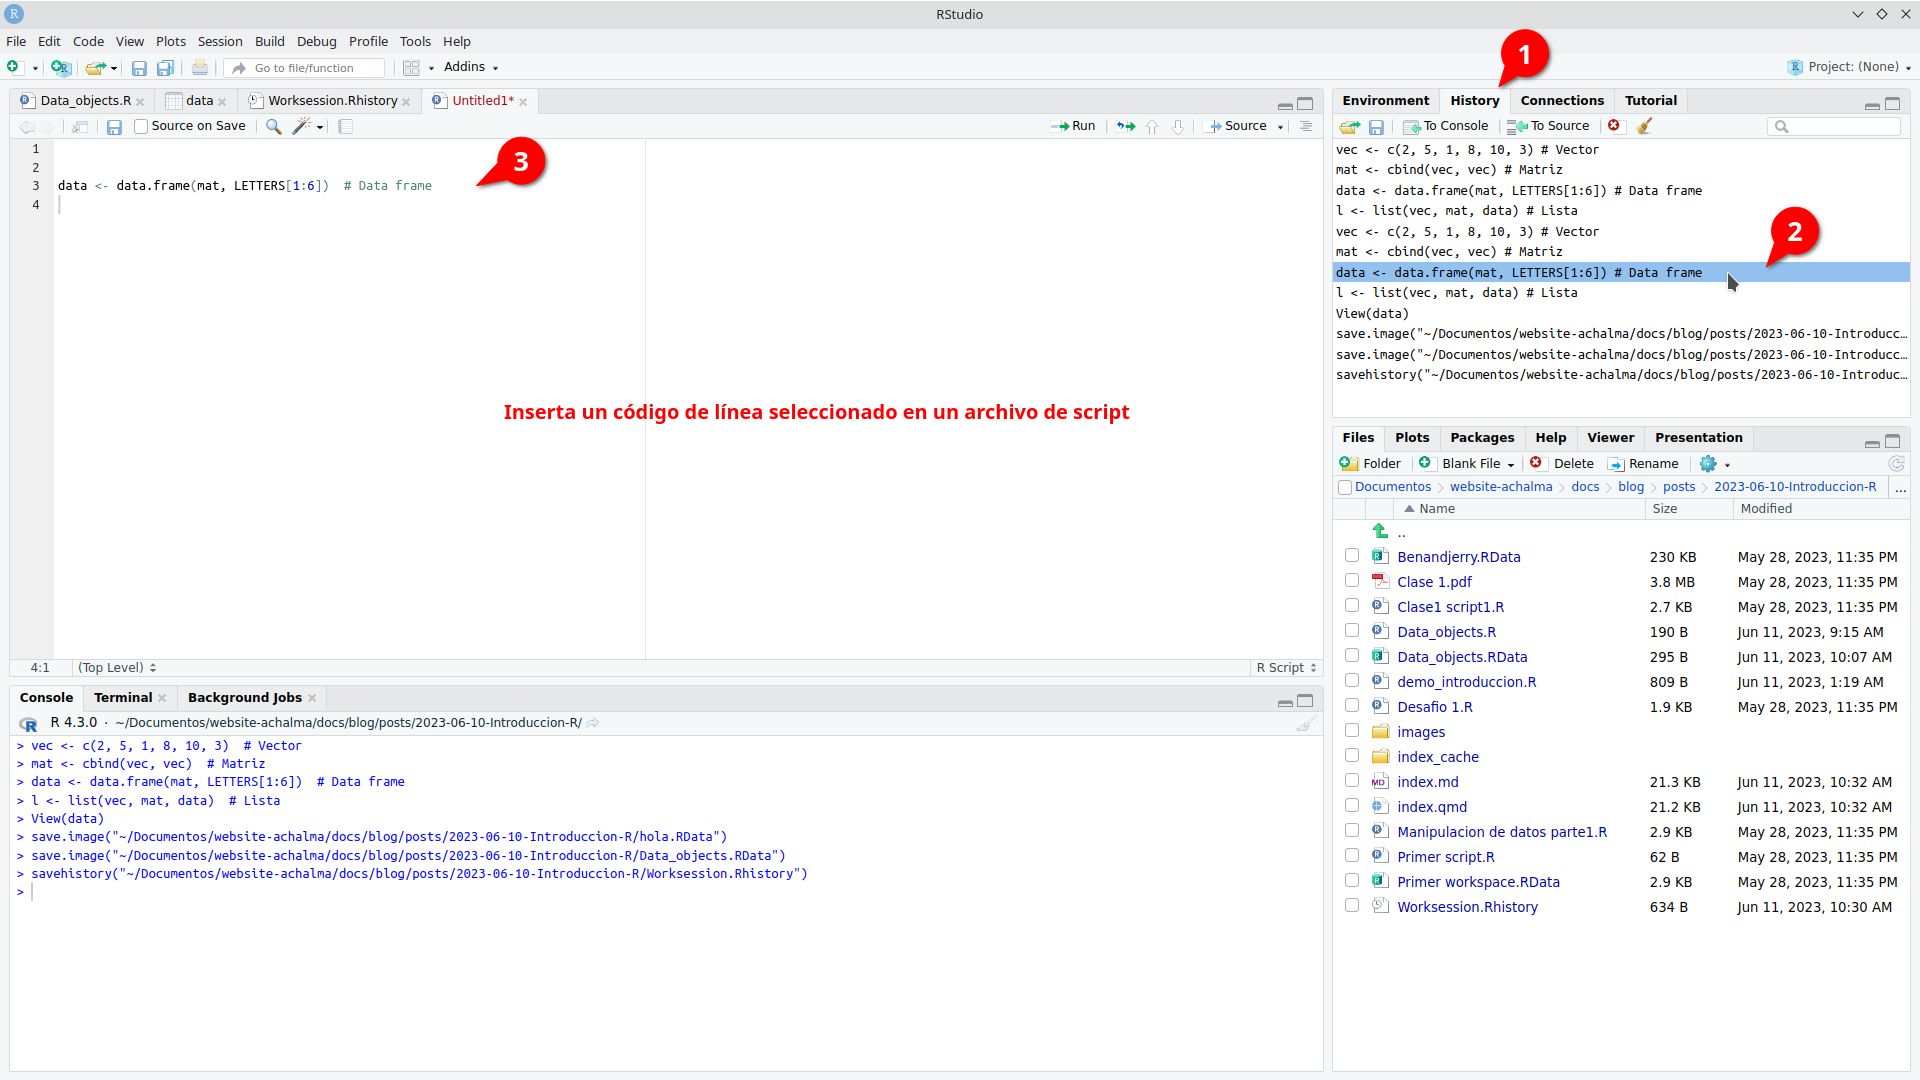
\includegraphics{2-Que-Ofrece-RStudio/images/Screenshot_20230611_103755.png}

\begin{quote}
¡Explora y aprovecha al máximo el espacio de trabajo y el historial en
RStudio para mejorar tu flujo de trabajo y aprovechar al máximo tus
comandos y objetos de datos!
\end{quote}

\hypertarget{lo-que-debemos-saber}{%
\chapter{Lo que debemos saber}\label{lo-que-debemos-saber}}

\hypertarget{tipos-de-datos}{%
\section{Tipos de datos}\label{tipos-de-datos}}

En R, es fundamental comprender los diferentes tipos de datos
disponibles. A continuación, exploraremos los tres tipos básicos de
datos en R y cómo se utilizan en la programación.

\hypertarget{tipos-de-datos-numuxe9ricos}{%
\subsection{1. Tipos de datos
numéricos}\label{tipos-de-datos-numuxe9ricos}}

Los datos numéricos en R se dividen en dos tipos principales:

\begin{enumerate}
\def\labelenumi{\alph{enumi}.}
\item
  Números reales, se conoce como \texttt{double}. Estos son los números
  más comunes y se utilizan para representar valores decimales. Por
  ejemplo, 3.14 y 2.71828 son números reales en R. La precisión de los
  números reales en R depende de la máquina en la que se ejecuta el
  programa.
\item
  Números enteros, se conoce como \texttt{integer}. Estos son números
  que no contienen decimales y se utilizan para representar valores
  enteros. Por ejemplo, 1, 2, -5 son ejemplos de números enteros en R.
  Los números enteros se utilizan cuando no se requiere precisión
  decimal.
\end{enumerate}

\hypertarget{tipo-de-datos-luxf3gico}{%
\subsection{2. Tipo de datos lógico}\label{tipo-de-datos-luxf3gico}}

El tipo de dato lógico en R se conoce como \texttt{booleano}. Este tipo
de dato puede tener uno de dos valores: TRUE o FALSE. Los valores
booleanos se utilizan principalmente para realizar operaciones de
comparación y evaluación lógica en los programas. Por ejemplo, se puede
usar una expresión lógica para verificar si una condición es verdadera o
falsa.

\hypertarget{tipo-de-datos-caruxe1cter}{%
\subsection{3. Tipo de datos carácter}\label{tipo-de-datos-caruxe1cter}}

El tipo de dato carácter en R se utiliza para almacenar letras
\texttt{text} y símbolos \texttt{strings}. Los datos de tipo carácter se
definen utilizando comillas simples ('`) o comillas dobles (````). Por
ejemplo,''Hola'' y 'RStudio' son ejemplos de datos de tipo carácter en
R. Los datos de tipo carácter se utilizan con frecuencia para almacenar
texto legible por humanos, como nombres, descripciones o mensajes.

\begin{quote}
Es importante comprender estos tipos de datos en R, ya que nos permiten
manipular y realizar operaciones en los datos de manera adecuada. Cada
tipo de dato tiene sus propias características y funciones asociadas que
nos permiten realizar tareas específicas en la programación.
\end{quote}

\hypertarget{estructura-de-datos}{%
\section{Estructura de datos}\label{estructura-de-datos}}

Las estructuras de datos nos permiten organizar y manipular la
información de manera eficiente. A continuación, exploraremos las
principales estructuras de datos disponibles en R y cómo se utilizan en
la programación.

\hypertarget{escalar}{%
\subsection{1. Escalar}\label{escalar}}

Un escalar es un dato individual, como un número o una palabra, que no
está agrupado con otros elementos. En R, los escalares pueden ser de
diferentes tipos de datos, como numéricos, lógicos o caracteres. Estos
datos se utilizan cuando solo necesitamos almacenar una única
observación.

\hypertarget{vector}{%
\subsection{2. Vector}\label{vector}}

Un vector es una colección ordenada de elementos del mismo tipo de dato.
Puede contener números, valores lógicos o caracteres. En R, los vectores
son utilizados para almacenar conjuntos de datos relacionados. Por
ejemplo, podemos tener un vector de edades o un vector de nombres. Los
vectores son una de las estructuras de datos más utilizadas en R y nos
permiten realizar operaciones y cálculos de manera eficiente.

\textbf{Vectores}

Concatenación de elementos con \textbf{\texttt{c()}}: Se utiliza la
función \texttt{c()} para concatenar elementos y crear vectores en R.

\begin{Shaded}
\begin{Highlighting}[]
\FunctionTok{c}\NormalTok{(}\FloatTok{0.5}\NormalTok{, }\FloatTok{0.6}\NormalTok{, }\FloatTok{0.25}\NormalTok{) }\CommentTok{\# números decimales (double)}
\FunctionTok{c}\NormalTok{(9L, 10L, 11L, 12L, 13L) }\CommentTok{\# números enteros (integer)}
\FunctionTok{c}\NormalTok{(}\DecValTok{9}\SpecialCharTok{:}\DecValTok{13}\NormalTok{) }\CommentTok{\# secuencia de números enteros (integer sequence)}
\FunctionTok{c}\NormalTok{(}\ConstantTok{TRUE}\NormalTok{, }\ConstantTok{FALSE}\NormalTok{, }\ConstantTok{FALSE}\NormalTok{) }\CommentTok{\# valores lógicos (logical)}
\FunctionTok{c}\NormalTok{(}\DecValTok{1} \SpecialCharTok{+}\NormalTok{ 0i, }\DecValTok{2} \SpecialCharTok{+}\NormalTok{ 4i) }\CommentTok{\# números complejos (complex)}
\FunctionTok{c}\NormalTok{(}\StringTok{"a"}\NormalTok{, }\StringTok{"b"}\NormalTok{, }\StringTok{"c"}\NormalTok{) }\CommentTok{\# caracteres (character)}
\end{Highlighting}
\end{Shaded}

\textbf{Acciones con vectores}

\begin{enumerate}
\def\labelenumi{\arabic{enumi}.}
\item
  Asignar los vectores a nombres:

  Creamos un vector llamado ``dbl'' que contiene los números decimales
  0.5, 0.6 y 0.25.

\begin{Shaded}
\begin{Highlighting}[]
\NormalTok{dbl }\OtherTok{\textless{}{-}} \FunctionTok{c}\NormalTok{(}\FloatTok{0.5}\NormalTok{, }\FloatTok{0.6}\NormalTok{, }\FloatTok{0.25}\NormalTok{)}
\end{Highlighting}
\end{Shaded}

  Creamos un vector llamado ``chr'' que contiene los caracteres ``a'',
  ``b'' y ``c''.

\begin{Shaded}
\begin{Highlighting}[]
\NormalTok{chr }\OtherTok{\textless{}{-}} \FunctionTok{c}\NormalTok{(}\StringTok{"a"}\NormalTok{, }\StringTok{"b"}\NormalTok{, }\StringTok{"c"}\NormalTok{)}
\end{Highlighting}
\end{Shaded}
\item
  Imprimir los vectores ``dbl'' y ``chr'' en la consola:

  Visualizamos en la consola el contenido del vector ``dbl'', que son
  los números decimales 0.5, 0.6 y 0.25.

\begin{Shaded}
\begin{Highlighting}[]
\NormalTok{dbl}
\end{Highlighting}
\end{Shaded}

  Visualizamos en la consola el contenido del vector ``chr'', que son
  los caracteres ``a'', ``b'' y ``c''.

\begin{Shaded}
\begin{Highlighting}[]
\NormalTok{chr}
\end{Highlighting}
\end{Shaded}
\item
  Verificar el número de elementos en ``dbl'' y ``chr'':

  Calculamos y mostramos en la consola la longitud del vector ``dbl'',
  que es 3.

\begin{Shaded}
\begin{Highlighting}[]
\FunctionTok{length}\NormalTok{(dbl)}
\end{Highlighting}
\end{Shaded}

  Calculamos y mostramos en la consola la longitud del vector ``chr'',
  que es 3.

\begin{Shaded}
\begin{Highlighting}[]
\FunctionTok{length}\NormalTok{(chr)}
\end{Highlighting}
\end{Shaded}
\item
  Verificar el tipo de dato de ``dbl'' y ``chr'':

  Visualizamos en la consola el tipo de dato del vector ``dbl'', que es
  ``double'' (números decimales).

\begin{Shaded}
\begin{Highlighting}[]
\FunctionTok{typeof}\NormalTok{(dbl)}
\end{Highlighting}
\end{Shaded}

  Visualizamos en la consola el tipo de dato del vector ``chr'', que es
  ``character'' (caracteres).

\begin{Shaded}
\begin{Highlighting}[]
\FunctionTok{typeof}\NormalTok{(chr)}
\end{Highlighting}
\end{Shaded}
\item
  Combinar dos vectores:

  Se puede combinar el vector ``dbl'' consigo mismo utilizando la
  función ``c()'', creando un nuevo vector que contiene los elementos
  duplicados del vector original.

\begin{Shaded}
\begin{Highlighting}[]
\FunctionTok{c}\NormalTok{(dbl, dbl)}
\end{Highlighting}
\end{Shaded}

  Tambien se puede combina el vector ``dbl'' con el vector ``chr''
  utilizando la función ``c()'', creando un nuevo vector que contiene
  los elementos de ambos vectores concatenados.

\begin{Shaded}
\begin{Highlighting}[]
\FunctionTok{c}\NormalTok{(dbl, chr)}
\end{Highlighting}
\end{Shaded}
\end{enumerate}

\begin{tcolorbox}[enhanced jigsaw, colframe=quarto-callout-note-color-frame, opacityback=0, left=2mm, breakable, bottomrule=.15mm, coltitle=black, bottomtitle=1mm, toptitle=1mm, titlerule=0mm, title=\textcolor{quarto-callout-note-color}{\faInfo}\hspace{0.5em}{Nota}, arc=.35mm, toprule=.15mm, colback=white, leftrule=.75mm, rightrule=.15mm, opacitybacktitle=0.6, colbacktitle=quarto-callout-note-color!10!white]

El cambio automático del tipo de datos del vector resultante se denomina
coerción. La coerción garantiza que se mantiene el mismo tipo de datos
para cada elemento del vector.

\end{tcolorbox}

\textbf{Operaciones aritméticas con vectores}

\begin{enumerate}
\def\labelenumi{\arabic{enumi}.}
\item
  Definamos dos nuevos vectores numéricos llamados \texttt{a} y
  \texttt{b} con 4 elementos cada uno:

\begin{Shaded}
\begin{Highlighting}[]
\NormalTok{a }\OtherTok{\textless{}{-}} \FunctionTok{c}\NormalTok{(}\DecValTok{1}\NormalTok{, }\DecValTok{2}\NormalTok{, }\DecValTok{3}\NormalTok{, }\DecValTok{4}\NormalTok{)}
\NormalTok{b }\OtherTok{\textless{}{-}} \FunctionTok{c}\NormalTok{(}\DecValTok{10}\NormalTok{, }\DecValTok{20}\NormalTok{, }\DecValTok{30}\NormalTok{, }\DecValTok{40}\NormalTok{)}
\end{Highlighting}
\end{Shaded}
\item
  Realizamos una multiplicación escalar de \texttt{a} por 5, lo que
  significa que cada elemento en \texttt{a} se multiplica por 5:

\begin{Shaded}
\begin{Highlighting}[]
\NormalTok{a }\SpecialCharTok{*} \DecValTok{5}
\end{Highlighting}
\end{Shaded}
\item
  Realizamos una multiplicación de vectores entre \texttt{a} y
  \texttt{b}, lo que implica multiplicar cada elemento en \texttt{a} por
  el elemento correspondiente en \texttt{b}:

\begin{Shaded}
\begin{Highlighting}[]
\NormalTok{a }\SpecialCharTok{*}\NormalTok{ b}
\end{Highlighting}
\end{Shaded}
\item
  Creamos un nuevo vector numérico llamado \texttt{v} con longitud 5.

\begin{Shaded}
\begin{Highlighting}[]
\NormalTok{v }\OtherTok{\textless{}{-}} \FunctionTok{c}\NormalTok{(}\FloatTok{1.1}\NormalTok{, }\FloatTok{1.2}\NormalTok{, }\FloatTok{1.3}\NormalTok{, }\FloatTok{1.4}\NormalTok{, }\FloatTok{1.5}\NormalTok{)}
\NormalTok{a }\SpecialCharTok{*}\NormalTok{ v}
\end{Highlighting}
\end{Shaded}
\end{enumerate}

\begin{tcolorbox}[enhanced jigsaw, colframe=quarto-callout-note-color-frame, opacityback=0, left=2mm, breakable, bottomrule=.15mm, coltitle=black, bottomtitle=1mm, toptitle=1mm, titlerule=0mm, title=\textcolor{quarto-callout-note-color}{\faInfo}\hspace{0.5em}{Nota}, arc=.35mm, toprule=.15mm, colback=white, leftrule=.75mm, rightrule=.15mm, opacitybacktitle=0.6, colbacktitle=quarto-callout-note-color!10!white]

Las operaciones aritméticas de los vectores se realizan por elementos.
si dos vectores no tienen la misma longitud, el vector más corto se
reciclará para que coincida con el más largo (en este caso, se vuelve a
utilizar el primer elemento de a).

\end{tcolorbox}

\hypertarget{matriz}{%
\subsection{3. Matriz}\label{matriz}}

Una matriz es una estructura bidimensional que contiene elementos
organizados en filas y columnas. Todos los elementos de una matriz deben
ser del mismo tipo de dato. Las matrices son útiles para almacenar datos
tabulares, como una tabla de datos con variables en filas y
observaciones en columnas. En R, podemos realizar operaciones
matriciales y manipular los datos de manera eficiente utilizando esta
estructura.

\textbf{Matrices}

\begin{enumerate}
\def\labelenumi{\arabic{enumi}.}
\item
  Combinamos los vectores \texttt{a} y \texttt{b}, definidas
  anteriormente, por columnas utilizando la función \texttt{cbind()}:

\begin{Shaded}
\begin{Highlighting}[]
\NormalTok{A }\OtherTok{\textless{}{-}} \FunctionTok{cbind}\NormalTok{(a, b)}
\NormalTok{A}
\end{Highlighting}
\end{Shaded}

  Esta opción combina los vectores \texttt{a} y \texttt{b} por columnas,
  creando una matriz \texttt{A} donde los elementos de \texttt{a} forman
  la primera columna y los elementos de \texttt{b} forman la segunda
  columna.
\item
  Combinamos los vectores \texttt{a} y \texttt{b} por filas utilizando
  la función \texttt{rbind()}:

\begin{Shaded}
\begin{Highlighting}[]
\NormalTok{B }\OtherTok{\textless{}{-}} \FunctionTok{rbind}\NormalTok{(a, b)}
\NormalTok{B}
\end{Highlighting}
\end{Shaded}

  En esta opción, los vectores \texttt{a} y \texttt{b} se combinan por
  filas para crear una matriz \texttt{B}. Los elementos de \texttt{a}
  forman la primera fila y los elementos de \texttt{b} forman la segunda
  fila.
\item
  Creamos una matriz a partir de los elementos de vector \texttt{a}
  utilizando la función \texttt{matrix()}:

\begin{Shaded}
\begin{Highlighting}[]
\NormalTok{A }\OtherTok{\textless{}{-}} \FunctionTok{matrix}\NormalTok{(a, }\AttributeTok{ncol =} \DecValTok{2}\NormalTok{, }\AttributeTok{nrow =} \DecValTok{2}\NormalTok{)}
\NormalTok{A}
\end{Highlighting}
\end{Shaded}

  Aquí se utiliza la función \texttt{matrix()} para crear una matriz
  \texttt{A} a partir de los elementos del vector \texttt{a}. Se
  especifica que la matriz tendrá 2 columnas y 2 filas. Los argumentos
  nrow y ncol indican el número de filas y el número de columnas de que
  consta la matriz resultante.
\item
  Para 4 elementos y ncol =2 la matriz sólo puede tener 2 filas. Por lo
  tanto no es necesario especificar ambos argumentos

\begin{Shaded}
\begin{Highlighting}[]
\NormalTok{A }\OtherTok{\textless{}{-}} \FunctionTok{matrix}\NormalTok{(a, }\AttributeTok{ncol =} \DecValTok{2}\NormalTok{)}
\NormalTok{A}
\end{Highlighting}
\end{Shaded}

  En esta variante, se crea una matriz \texttt{A} con 2 columnas y se
  ajusta automáticamente el número de filas según la longitud del vector
  \texttt{a}.
\item
  Por defecto la matriz se rellena columna a columna (R trata
  internamente un objeto matriz como vector columna). si la matriz debe
  rellenarse fila a fila se requiere el argumento
  \texttt{byrow\ =\ TRUE}

\begin{Shaded}
\begin{Highlighting}[]
\NormalTok{B }\OtherTok{\textless{}{-}} \FunctionTok{matrix}\NormalTok{(a, }\AttributeTok{ncol =} \DecValTok{2}\NormalTok{, }\AttributeTok{byrow =} \ConstantTok{TRUE}\NormalTok{)}
\NormalTok{B}
\end{Highlighting}
\end{Shaded}

  En esta opción, se crea una matriz \texttt{B} con 2 columnas y se
  especifica que los elementos del vector \texttt{a} se distribuirán por
  filas \texttt{byrow\ =\ TRUE}, es decir, los primeros elementos de
  \texttt{a} formarán la primera fila, los siguientes elementos formarán
  la segunda fila, y así sucesivamente.
\end{enumerate}

\textbf{Acciones con matrices}

\begin{enumerate}
\def\labelenumi{\arabic{enumi}.}
\item
  Verificamos el número de filas de la matriz \texttt{A} utilizando la
  función \texttt{nrow()}:

\begin{Shaded}
\begin{Highlighting}[]
\FunctionTok{nrow}\NormalTok{(A)}
\end{Highlighting}
\end{Shaded}

  Esta línea de código devuelve el número de filas de la matriz
  \texttt{A}.
\item
  Verificamos el número de columnas de la matriz \texttt{A} utilizando
  la función \texttt{ncol()}:

\begin{Shaded}
\begin{Highlighting}[]
\FunctionTok{ncol}\NormalTok{(A)}
\end{Highlighting}
\end{Shaded}

  Aquí se obtiene el número de columnas de la matriz \texttt{A}.
\item
  Verificamos la dimensión (número de filas y columnas) de la matriz
  \texttt{A} utilizando la función \texttt{dim()}:

\begin{Shaded}
\begin{Highlighting}[]
\FunctionTok{dim}\NormalTok{(A)}
\end{Highlighting}
\end{Shaded}

  Esta línea de código devuelve la dimensión de la matriz \texttt{A} en
  formato \texttt{{[}nrow,\ ncol{]}}.
\item
  Combinamos dos matrices \texttt{A} por columnas utilizando la función
  \texttt{cbind()} y almacenamos el resultado en \texttt{D.wide}:

\begin{Shaded}
\begin{Highlighting}[]
\NormalTok{D.wide }\OtherTok{\textless{}{-}} \FunctionTok{cbind}\NormalTok{(A, A)}
\NormalTok{D.wide}
\end{Highlighting}
\end{Shaded}

  En esta línea se crea una nueva matriz \texttt{D.wide} que combina las
  matrices \texttt{A} y \texttt{A} por columnas.
\item
  Combinamos dos matrices \texttt{A} por filas utilizando la función
  \texttt{rbind()} y almacenamos el resultado en \texttt{D.long}:

\begin{Shaded}
\begin{Highlighting}[]
\NormalTok{D.long }\OtherTok{\textless{}{-}} \FunctionTok{rbind}\NormalTok{(A, A)}
\NormalTok{D.long}
\end{Highlighting}
\end{Shaded}

  Aquí se crea una nueva matriz \texttt{D.long} que combina las matrices
  \texttt{A} y \texttt{A} por filas.
\item
  Combinamos las matrices \texttt{D.wide} y \texttt{D.long} por columnas
  utilizando la función \texttt{cbind()} y almacenamos el resultado en
  \texttt{D}:

\begin{Shaded}
\begin{Highlighting}[]
\CommentTok{\# D \textless{}{-} cbind(D.wide, D.long)}
\end{Highlighting}
\end{Shaded}

  En esta línea se crea una nueva matriz \texttt{D} que combina las
  matrices \texttt{D.wide} y \texttt{D.long} por columnas.
\end{enumerate}

\textbf{Operaciones aritméticas con matrices}

\begin{enumerate}
\def\labelenumi{\arabic{enumi}.}
\item
  Suma de la matriz \texttt{B} consigo misma utilizando el operador
  \texttt{+}:

\begin{Shaded}
\begin{Highlighting}[]
\NormalTok{B }\SpecialCharTok{+}\NormalTok{ B}
\end{Highlighting}
\end{Shaded}

  Esta línea de código realiza la suma de la matriz \texttt{B} con ella
  misma.
\item
  Multiplicación escalar de la matriz \texttt{B} por 2 utilizando el
  operador \texttt{*}:

\begin{Shaded}
\begin{Highlighting}[]
\NormalTok{B }\SpecialCharTok{*} \DecValTok{2}
\end{Highlighting}
\end{Shaded}

  Aquí se realiza la multiplicación de cada elemento de la matriz
  \texttt{B} por 2.
\item
  Multiplicación elemento a elemento de la matriz \texttt{B} consigo
  misma y almacenar el resultado en \texttt{a}:

\begin{Shaded}
\begin{Highlighting}[]
\NormalTok{a }\OtherTok{\textless{}{-}}\NormalTok{ B }\SpecialCharTok{*}\NormalTok{ B}
\NormalTok{a}
\end{Highlighting}
\end{Shaded}

  En esta línea se realiza la multiplicación elemento a elemento de la
  matriz \texttt{B} con ella misma, y el resultado se almacena en la
  matriz \texttt{a}.
\item
  Multiplicación de matrices utilizando el operador \texttt{\%*\%}:

\begin{Shaded}
\begin{Highlighting}[]
\NormalTok{C }\OtherTok{\textless{}{-}}\NormalTok{ B }\SpecialCharTok{\%*\%}\NormalTok{ B}
\NormalTok{C}
\end{Highlighting}
\end{Shaded}

  Aquí se realiza la multiplicación de matrices entre la matriz
  \texttt{B} y ella misma, y el resultado se almacena en la matriz
  \texttt{C}.
\end{enumerate}

\textbf{Otras operaciones con matrices:}

\begin{enumerate}
\def\labelenumi{\arabic{enumi}.}
\item
  Transposición de la matriz \texttt{D.wide} utilizando la función
  \texttt{t()}:

\begin{Shaded}
\begin{Highlighting}[]
\FunctionTok{t}\NormalTok{(D.wide)}
\end{Highlighting}
\end{Shaded}

  Esta línea de código transpone la matriz \texttt{D.wide}, es decir,
  intercambia las filas por columnas y viceversa.
\item
  Cálculo del determinante de la matriz \texttt{B} utilizando la función
  \texttt{det()}:

\begin{Shaded}
\begin{Highlighting}[]
\FunctionTok{det}\NormalTok{(B)}
\end{Highlighting}
\end{Shaded}

  Aquí se calcula el determinante de la matriz \texttt{B}.
\item
  Cálculo de la inversa de la matriz \texttt{B} utilizando la función
  \texttt{solve()} (solo si el determinante es diferente de 0):

\begin{Shaded}
\begin{Highlighting}[]
\FunctionTok{solve}\NormalTok{(B)}
\end{Highlighting}
\end{Shaded}

  En esta línea se calcula la inversa de la matriz \texttt{B}, siempre y
  cuando el determinante sea diferente de 0.
\item
  Cálculo de los valores propios (eigenvalues) de una matriz cuadrada y
  simétrica utilizando la función \texttt{eigen()}:

\begin{Shaded}
\begin{Highlighting}[]
\FunctionTok{eigen}\NormalTok{(B)}
\end{Highlighting}
\end{Shaded}

  Aquí se calculan los valores propios de la matriz \texttt{B}. Esta
  operación solo es aplicable a matrices cuadradas y simétricas.
\end{enumerate}

\hypertarget{data-frame}{%
\subsection{4. Data frame}\label{data-frame}}

Un data frame es una estructura similar a una matriz, pero más flexible.
Puede contener columnas con diferentes tipos de datos, lo que lo hace
ideal para almacenar conjuntos de datos heterogéneos. Los data frames
son muy utilizados en el análisis de datos, ya que nos permiten
manipular y explorar datos de manera eficiente. Podemos realizar
operaciones de filtrado, selección y transformación en los data frames
para obtener información significativa.

\textbf{Creación del data frame:}

\begin{enumerate}
\def\labelenumi{\arabic{enumi}.}
\item
  Creamos vectores con diferentes tipos de datos, como números decimales
  (\texttt{dbl}), números enteros (\texttt{int}), valores lógicos
  (\texttt{lgl}) y caracteres (\texttt{chr}):

\begin{Shaded}
\begin{Highlighting}[]
\NormalTok{dbl }\OtherTok{\textless{}{-}} \FunctionTok{c}\NormalTok{(}\FloatTok{0.5}\NormalTok{, }\FloatTok{0.6}\NormalTok{, }\FloatTok{0.25}\NormalTok{, }\FloatTok{1.2}\NormalTok{, }\FloatTok{0.333}\NormalTok{) }\CommentTok{\# números decimales (double)}
\NormalTok{int }\OtherTok{\textless{}{-}} \FunctionTok{c}\NormalTok{(9L, 10L, 11L, 12L, 13L) }\CommentTok{\# números enteros (integer)}
\NormalTok{lgl }\OtherTok{\textless{}{-}} \FunctionTok{c}\NormalTok{(}\ConstantTok{TRUE}\NormalTok{, }\ConstantTok{FALSE}\NormalTok{, }\ConstantTok{FALSE}\NormalTok{, }\ConstantTok{TRUE}\NormalTok{, }\ConstantTok{TRUE}\NormalTok{) }\CommentTok{\# valores lógicos (logical)}
\NormalTok{chr }\OtherTok{\textless{}{-}} \FunctionTok{c}\NormalTok{(}\StringTok{"a"}\NormalTok{, }\StringTok{"b"}\NormalTok{, }\StringTok{"c"}\NormalTok{, }\StringTok{"d"}\NormalTok{, }\StringTok{"e"}\NormalTok{) }\CommentTok{\# caracteres (character)}
\end{Highlighting}
\end{Shaded}

  Cada vector tiene elementos que representan valores de su respectivo
  tipo de dato.
\item
  Utilizamos la función \texttt{data.frame()} para combinar los vectores
  en un data frame llamado \texttt{df}:

\begin{Shaded}
\begin{Highlighting}[]
\NormalTok{df }\OtherTok{\textless{}{-}} \FunctionTok{data.frame}\NormalTok{(dbl, int, lgl, chr)}
\end{Highlighting}
\end{Shaded}

  El data frame \texttt{df} se crea utilizando los vectores
  \texttt{dbl}, \texttt{int}, \texttt{lgl} y \texttt{chr} como columnas.
\item
  Mostamos el contenido del data frame en la consola:

\begin{Shaded}
\begin{Highlighting}[]
\NormalTok{df}
\end{Highlighting}
\end{Shaded}

  Esto imprime el contenido del data frame \texttt{df}.
\end{enumerate}

\textbf{Acciones con data frames:}

\begin{enumerate}
\def\labelenumi{\arabic{enumi}.}
\item
  Verificamos el número de filas del data frame utilizando la función
  \texttt{nrow()}:

\begin{Shaded}
\begin{Highlighting}[]
\FunctionTok{nrow}\NormalTok{(df)}
\end{Highlighting}
\end{Shaded}

  Esta línea de código devuelve el número de filas en el data frame
  \texttt{df}.
\item
  Verificamos el número de columnas del data frame utilizando la función
  \texttt{ncol()}:

\begin{Shaded}
\begin{Highlighting}[]
\FunctionTok{ncol}\NormalTok{(df)}
\end{Highlighting}
\end{Shaded}

  Aquí se obtiene el número de columnas en el data frame \texttt{df}.
\item
  Verificamos la dimensión (número de filas y columnas) del data frame
  utilizando la función \texttt{dim()}:

\begin{Shaded}
\begin{Highlighting}[]
\FunctionTok{dim}\NormalTok{(df)}
\end{Highlighting}
\end{Shaded}

  Esta línea de código devuelve la dimensión del data frame \texttt{df}
  en formato \texttt{{[}nrow,\ ncol{]}}, es decir, el número de filas y
  columnas que tiene el data frame.
\end{enumerate}

\hypertarget{lista}{%
\subsection{5. Lista}\label{lista}}

Una lista es una estructura de datos genérica que puede contener
diferentes objetos, como vectores, matrices, data frames o incluso otras
listas. A diferencia de las otras estructuras, las listas no tienen
restricciones en cuanto a los tipos de datos o la longitud de los
componentes individuales. Las listas son muy flexibles y se utilizan
cuando necesitamos almacenar objetos de diferentes tipos o estructuras
complejas.

\textbf{Creación de la lista}

\begin{enumerate}
\def\labelenumi{\arabic{enumi}.}
\item
  Creamos una variable \texttt{a} que contiene un \textbf{escalar} de
  tipo entero (\texttt{1L}):

\begin{Shaded}
\begin{Highlighting}[]
\NormalTok{a }\OtherTok{\textless{}{-}}\NormalTok{ 1L}
\end{Highlighting}
\end{Shaded}
\item
  Creamos un \textbf{vector numérico} \texttt{dbl} con 5 elementos:

\begin{Shaded}
\begin{Highlighting}[]
\NormalTok{dbl }\OtherTok{\textless{}{-}} \FunctionTok{c}\NormalTok{(}\FloatTok{0.5}\NormalTok{, }\FloatTok{0.6}\NormalTok{, }\FloatTok{0.25}\NormalTok{, }\FloatTok{1.2}\NormalTok{, }\FloatTok{0.333}\NormalTok{)}
\end{Highlighting}
\end{Shaded}
\item
  Creamos un \textbf{vector de caracteres} \texttt{chr} con 3 elementos:

\begin{Shaded}
\begin{Highlighting}[]
\NormalTok{chr }\OtherTok{\textless{}{-}} \FunctionTok{c}\NormalTok{(}\StringTok{"a"}\NormalTok{, }\StringTok{"b"}\NormalTok{, }\StringTok{"c"}\NormalTok{)}
\end{Highlighting}
\end{Shaded}
\item
  Creamos un vector \texttt{v} con 4 elementos de tipo numérico:

\begin{Shaded}
\begin{Highlighting}[]
\NormalTok{v }\OtherTok{\textless{}{-}} \FunctionTok{c}\NormalTok{(}\FloatTok{1.1}\NormalTok{, }\FloatTok{1.2}\NormalTok{, }\FloatTok{1.3}\NormalTok{, }\FloatTok{1.4}\NormalTok{)}
\end{Highlighting}
\end{Shaded}
\item
  Creamos una matriz \texttt{mat} de tamaño 2x2 a partir del vector
  \texttt{v}:

\begin{Shaded}
\begin{Highlighting}[]
\NormalTok{mat }\OtherTok{\textless{}{-}} \FunctionTok{matrix}\NormalTok{(v, }\AttributeTok{ncol =} \DecValTok{2}\NormalTok{)}
\end{Highlighting}
\end{Shaded}

  La matriz \texttt{mat} tiene 2 columnas y los elementos del vector
  \texttt{v} se llenan por columnas.
\item
  Creamos una lista \texttt{l} que contiene los elementos \texttt{a},
  \texttt{dbl}, \texttt{chr} y \texttt{mat}:

\begin{Shaded}
\begin{Highlighting}[]
\NormalTok{l }\OtherTok{\textless{}{-}} \FunctionTok{list}\NormalTok{(a, dbl, chr, mat)}
\end{Highlighting}
\end{Shaded}

  La lista \texttt{l} contiene estos elementos en ese orden.
\item
  Finalmente, visualizamos el contenido de la lista en la consola:

\begin{Shaded}
\begin{Highlighting}[]
\NormalTok{l}
\end{Highlighting}
\end{Shaded}

  Esto imprime el contenido de la lista \texttt{l}.
\end{enumerate}

\begin{quote}
Es importante comprender estas estructuras de datos en R, ya que nos
permiten organizar y manipular la información de manera efectiva. Cada
estructura tiene sus propias características y funciones asociadas que
nos facilitan el trabajo con los datos en la programación.
\end{quote}

\hypertarget{manipulaciuxf3n-de-datos}{%
\chapter{Manipulación de datos}\label{manipulaciuxf3n-de-datos}}

\bookmarksetup{startatroot}

\hypertarget{references}{%
\chapter*{References}\label{references}}
\addcontentsline{toc}{chapter}{References}

\markboth{References}{References}

\printbibliography[heading=none]

\cleardoublepage
\phantomsection
\addcontentsline{toc}{part}{Apéndices}
\appendix


\printbibliography[title=apendice]


\end{document}
